\documentclass[10pt,twoside]{book}

\usepackage{graphicx}
\usepackage{caption}
\usepackage{subcaption}
\usepackage{amsfonts}
\usepackage{amsmath}
\usepackage{xcolor}
\usepackage{array}
\usepackage{hyperref}
\hypersetup{
    colorlinks=true,
    linkcolor=blue,
    filecolor=magenta,      
    urlcolor=cyan
    }
\urlstyle{same}



\def\hideChapterSmoothingAndInterpolation{0}
\def\hideChapterRegistration{0}
\def\hideChapterModelBasedSegmentation{0}
\def\hideChapterNeuralNetworks{0}
\def\hideChapterAtlases{0}
\def\hideChapterValidation{0}



\begin{document}


\thispagestyle{empty}

\vspace*{\fill}

\begin{center}
{\huge \textbf{Medical Image Analysis}}\\*[2.5cm]
{\Large Koen Van Leemput}\\*[2.5cm]
{\large \today}

\end{center}

\vspace*{\fill}

\newpage

\vspace*{\fill}
\noindent
\copyright \ This work is licensed under CC BY 4.0
% \vspace*{\fill}


\thispagestyle{empty}


\frontmatter
\pagenumbering{roman}



\graphicspath{%
  {./figures/smoothingAndInterpolation/}%
  {./figures/registration/}%
  {./figures/modelBasedSegmentation/}%
  {./figures/neuralNets/}%
  {./figures/atlases/}%
  {./figures/validation/}%
  }

\tableofcontents

\clearpage


% Math notation stuff
\newcommand{\bldgr}[1]{{\mbox{\boldmath {${#1}$}}}} % Bold for lower-case Greek laters
\newcommand{\fat}[1]{\mathbf{#1}} % Bold for anything else
%\newcommand{\transp}{^\textrm{T}} % Transpose
\newcommand{\transp}{^\mathrm{T}} % Transpose
\newcommand{\N}{\mathcal N \mathnormal}


\mainmatter


\clearpage

\if\hideChapterSmoothingAndInterpolation0

\chapter{Smoothing and Interpolation}
\label{chap:smoothingAndInterpolation}

A fundamental prerequisite for solving many medical image analysis tasks is the ability to smooth and interpolate signals in two or three dimensions. In this chapter the basic principles of these techniques are reviewed.


\section{Linear regression}
\label{sec:linearRegression}

Let $\fat{x} = (x_1, \ldots, x_D )\transp$ denote the spatial position in a $D$-dimensional space. In medical imaging, $D$ is typically 2 or 3. 
%
Given $N$ measurements $\{t_n\}_{n=1}^N$ at locations $\{\fat{x}_n\}_{n=1}^N$, a frequent task is to predict the value $t$ at a new location $\fat{x}$.
%
% This can be constructing 
A simple model, known as \emph{linear regression}, uses the function value
$$
y( \fat{x}, \fat{w} ) = w_0 + w_1 x_1 + \ldots + w_D x_D
$$
as its prediction, where 
% $\fat{w} = (w_0, \ldots, w_D)\transp$ 
$w_0, \ldots, w_D$
are tunable weights that need to be estimated from the 
% $N$ 
available measurements.
%
A more general form uses nonlinear functions of the input locations instead:
$$
y( \fat{x}, \fat{w} ) = w_0 + \sum_{m=1}^{M-1} w_m \phi_m( \fat{x} )
,
$$
which greatly increases the flexibility of the model.
Here the functions $\phi_m(\fat{x})$ are known as \emph{basis functions}, and it is often convenient to define an additional ``dummy'' basis function 
$\phi_0(\fat{x})=1$, so that the model can be written as
\begin{equation}
y( \fat{x}, \fat{w} ) = \sum_{m=0}^{M-1} w_m \phi_m( \fat{x} ),
\label{eq:prediction}
\end{equation}
where $\fat{w} = (w_0, \ldots, w_{M-1})\transp$ are $M$ tunable parameters.

In order to find suitable values of the parameters of the model, the following energy can be minimized with respect to $\fat{w}$:
$$
E( \fat{w} ) = \sum_{n=1}^N 
               \left( t_n - \sum_{m=0}^{M-1} w_m \phi_m(\fat{x}_n) \right)^2
,               
$$
which simply sums of the squared distances between the measurements $t_n$ and the model's predictions $y(\fat{x}_n, \fat{w})$.
Taking the partial derivative with respect to parameter $w_m$ yields
$$
\frac{\partial E( \fat{w} ) }{ \partial w_m}
=
-2
\sum_{n=1}^N 
\left( t_n - \sum_{m=0}^{M-1} w_m \phi_m(\fat{x}_n) \right)
\phi_m(\fat{x}_n)
,
$$
so that the gradient is given by
$$
\nabla E( \fat{w} )
=
\left(
\begin{array}{c}
\frac{\partial E( \fat{w} ) }{ \partial w_0} \\
\vdots \\
\frac{\partial E( \fat{w} ) }{ \partial w_{M-1}}
\end{array}
\right)
=
-2
\bldgr{\Phi}\transp
\left( \fat{t} - \bldgr{\Phi} \fat{w} \right)
,
$$
where $\fat{t} = (t_1, \ldots, t_N)\transp$
is a vector stacking all measurements,
and 
\begin{equation}
\bldgr{\Phi} 
=
\left(
\begin{array}{cccc}
\phi_0( \fat{x}_1 ) & \phi_1( \fat{x}_1 ) & \hdots & \phi_{M-1}( \fat{x}_1 ) \\  
\phi_0( \fat{x}_2 ) & \phi_1( \fat{x}_2 ) & \hdots & \phi_{M-1}( \fat{x}_2 ) \\  
\vdots              & \vdots              & \ddots & \vdots  \\  
\phi_0( \fat{x}_N ) & \phi_1( \fat{x}_N ) & \hdots & \phi_{M-1}( \fat{x}_N ) \\  
\end{array}
\right)
\label{eq:Phi}
\end{equation}
is a $N \times M$ matrix containing the value of all the basis functions in each of the measurement locations.
Settings this gradient to zero gives 
$$
\bldgr{\Phi}\transp
\left( \fat{t} - \bldgr{\Phi} \fat{w} \right) 
= \fat{0}
$$
with solution 
\begin{equation}
\fat{w} =
\left( \bldgr{\Phi}\transp \bldgr{\Phi} \right)^{-1}
\bldgr{\Phi}\transp \fat{t}
\label{eq:coefficients}
.
\end{equation}
%
With these parameters, a prediction at a new location $\fat{x}$ is obtained by evaluating~\eqref{eq:prediction}.


\subsection{Regularization}

In some cases prior knowledge is available about the parameters $\fat{w}$ (for instance, that their values are typically small), or about the expected  behavior of $y(\fat{x}, \fat{w})$ (for instance that it is a smooth function). This can be taken into account by adding a regularization term to the energy, optimizing
\begin{equation}
E(\fat{w}) + \lambda \| \bldgr{\Omega} \fat{w} \|^2
\label{eq:regularization}
\end{equation}
instead. 
Here $\lambda$ is a parameter controlling the strength of the regularization, and
$\bldgr{\Omega}$ is a matrix chosen so that it penalizes undesirable values of $\fat{w}$. An example of $\bldgr{\Omega}$ could simply be the identify matrix, so that the regularization energy becomes 
$$
\| \fat{w} \|^2 = w_0^2 + \ldots + w_{M-1}^2
,
$$
which penalizes large values of $\fat{w}$. Other examples include 
$\bldgr{\Omega} = \bldgr{\Phi}$, so that large values of the \emph{predictions}
$\fat{\hat{t}} = \bldgr{\Phi} \fat{w}$
at the measurement locations 
%$\{\fat{x}\}_{n=1}^N$ 
are penalized; 
or even   
$\bldgr{\Omega} = \bldgr{\Gamma} \bldgr{\Phi}$, with $\bldgr{\Gamma}$ detecting rapid spatial fluctuations in 
$\fat{\hat{t}}$
%$\bldgr{\Phi} \fat{w}$ 
(e.g., first- or second-order finite differences).

Optimizing~\eqref{eq:regularization} with respect to $\fat{w}$, by setting its gradient to zero and solving for $\fat{w}$ as before, yields 
\begin{equation}
\fat{w} =
\left( \bldgr{\Phi}\transp \bldgr{\Phi} + \lambda \bldgr{\Omega}\transp \bldgr{\Omega} \right)^{-1}
\bldgr{\Phi}\transp \fat{t}
,
\label{eq:coefficientsWithRegularization}
\end{equation}
which is a straightforward extension of~\eqref{eq:coefficients}



\section{Smoothing and interpolation of 1D signals}
\label{sec:smoothingAndInterpolation1D}

Before addressing applications in two- or three-dimensional imaging problems, it is instructive to first study the one-dimensional (1D) setting. In this scenario, we are seeking functions of the form
\begin{equation}
y( x, \fat{w} ) = \sum_{m=0}^{M-1} w_m \phi_m( x ),
\label{eq:prediction1D}
\end{equation}
where $x$ is a scalar (a location in 1D space).
Furthermore, the 
$N$ 
measurement locations 
% $\{x_n\}_{n=1}^N$ 
lie on a regular grid with unit interval:
$$
x_n = n-1, \quad \forall n=1, \ldots, N,
$$
i.e., the signals $\fat{t}$ are 
% measured at consecutive integer locations.
1D ``images''.


%
In signal processing applications, the basis functions associated with the ``type II'' discrete cosine transform (DCT) often have useful analytical and numerical properties.
% \footnote{
In particular, they often allow to compress signals efficiently by discarding the highest frequencies; $\bldgr{\Phi} \fat{w}$ and $\bldgr{\Phi}\transp \fat{t}$ can be computed very quickly using the fast Fourier transform (FTT); and $\bldgr{\Phi}\transp\bldgr{\Phi} = \frac{N}{2} \fat{I}$.
% }. 
%
They are defined as follows:
\begin{equation}
\phi_m( x ) 
= 
\left( 
  \frac{1}{\sqrt{2}} \right)^{[m=0]}
  \cos\left( \pi m ( x + \frac{1}{2} ) / N 
\right)
\label{eq:DCTbasisFunctions}
,
\end{equation}
for frequencies $m=0, \ldots, M-1$, where $M \leq N$.
%
%
An example is shown in Fig.~\ref{fig:basisFunctions1D_DCT} for $M=5$. 

\begin{figure}
  \centering
  \begin{subfigure}{0.45\textwidth}
     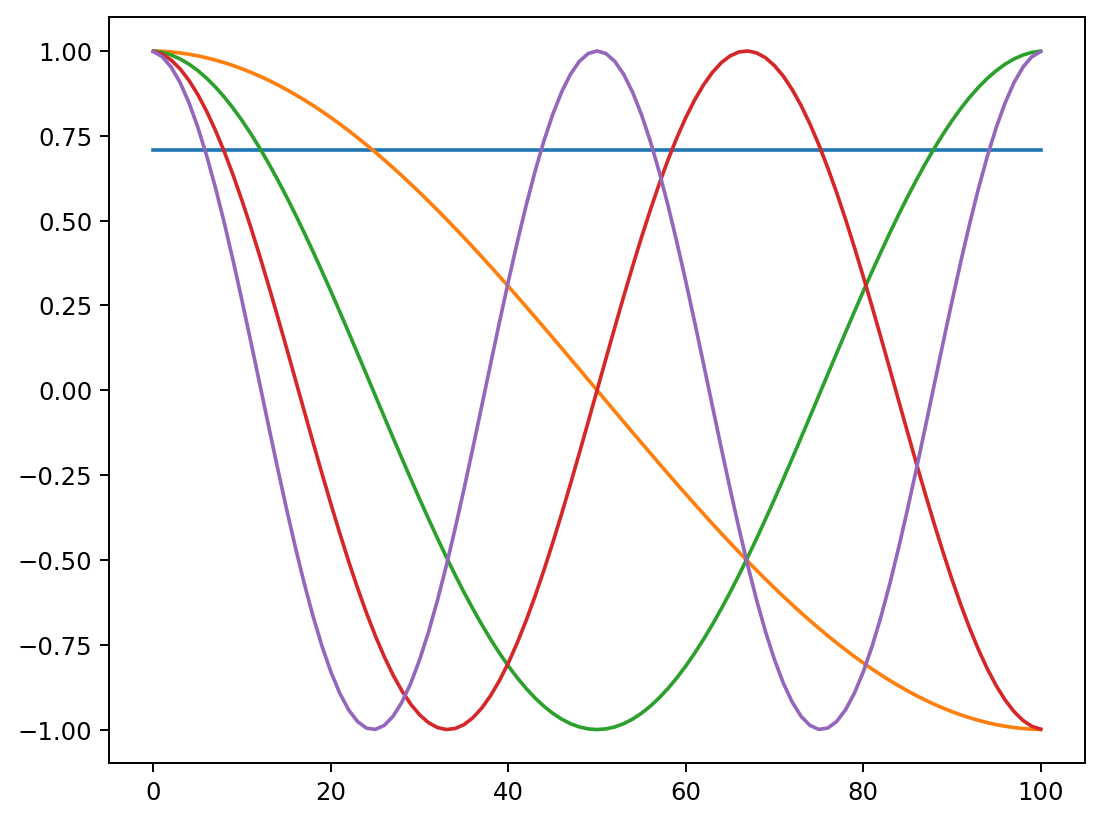
\includegraphics[width=\textwidth]{basisFunctions_type0}
     \caption{DCT}
     \label{fig:basisFunctions1D_DCT}
  \end{subfigure}
  \hfill
  \begin{subfigure}{0.45\textwidth}
     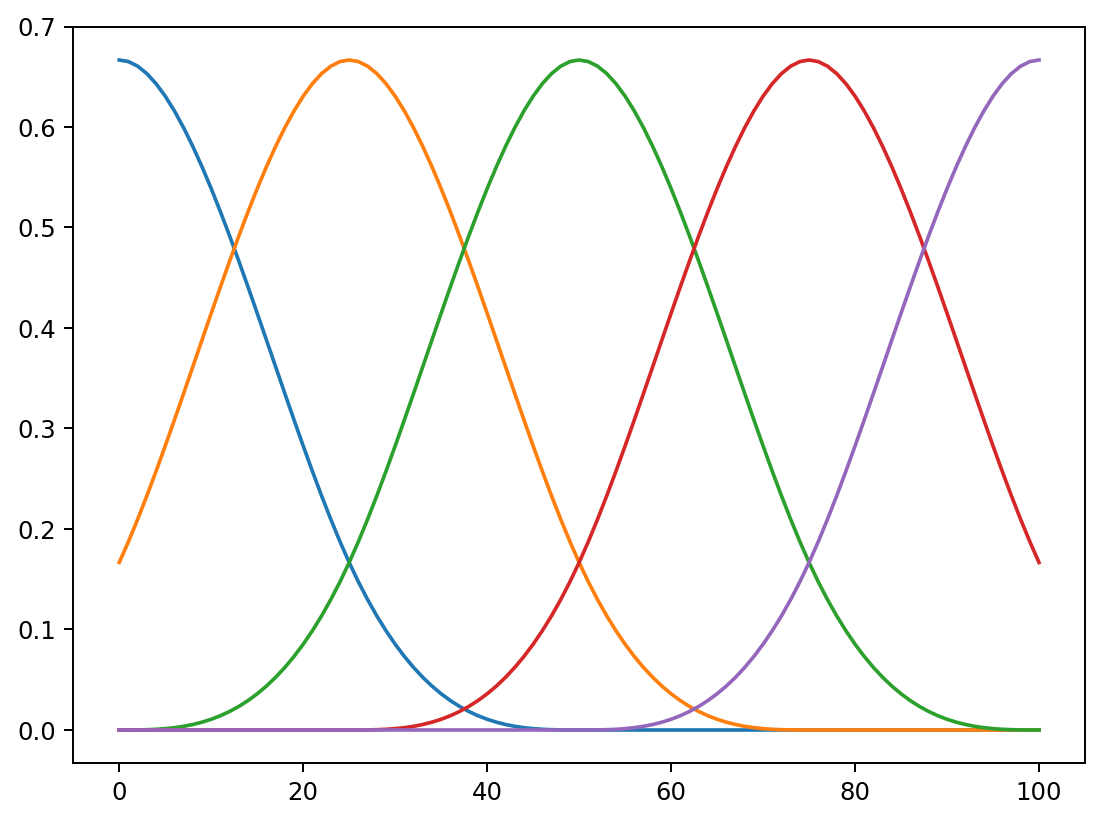
\includegraphics[width=\textwidth]{basisFunctions_type1}
     \caption{B-spline}
     \label{fig:basisFunctions1D_BSpline}
  \end{subfigure}
  \caption{Two sets of often-used basis functions ($M=5$).}
  %\label{fig:basisFunctions1D}
\end{figure}



Another set of useful basis functions are derived from B-splines, which are symmetrical functions constructed from the repeated convolution of a rectangular pulse $\beta^0$:
\begin{eqnarray*}
\beta^0( x ) 
& = &
\left\{
\begin{array}{ll}
1, & -\frac{1}{2} < x < \frac{1}{2} \\
\frac{1}{2}, & | x | = \frac{1}{2} \\
0, & \text{otherwise,}
\end{array}
\right. \\
\beta^p( x ) 
& = & 
\underbrace{
\left(
\beta^0 \ast \beta^0 \ast \cdots \ast \beta^0
\right)
}_{(p+1) \text{ times}}
(x)
.
\end{eqnarray*}
Here $p$ is called the \emph{order} of the B-spline, and 
% $f \ast g(x)$  
$\ast$ denotes a convolution:
$$
\left( f \ast g \right) (x ) = \int_{\tau = -\infty}^{\infty} f( \tau ) g( x - \tau ) \mathrm{d}\tau
.
$$
Often-used B-spline orders (e.g, for interpolation) are $p=1$:
$$
\beta^1(x) 
= 
\left\{
\begin{array}{ll}
1 - |x|, & | x | < 1 \\
0, & \text{otherwise,}
\end{array}
\right.
$$
and $p=3$ (``cubic'' B-spline):
$$
\beta^3(x) 
= 
\left\{
\begin{array}{ll}
\frac{2}{3} - |x|^2 + \frac{|x|^3}{2}, & | x | < 1 \\
\frac{(2 - |x|)^3}{6}, & 1 \leq |x| < 2 \\
0, & \text{otherwise.}
\end{array}
\right.
$$
B-splines of order zero, one and three are illustrated in Fig.~\ref{fig:Bsplines}.

\begin{figure}
  \centering
  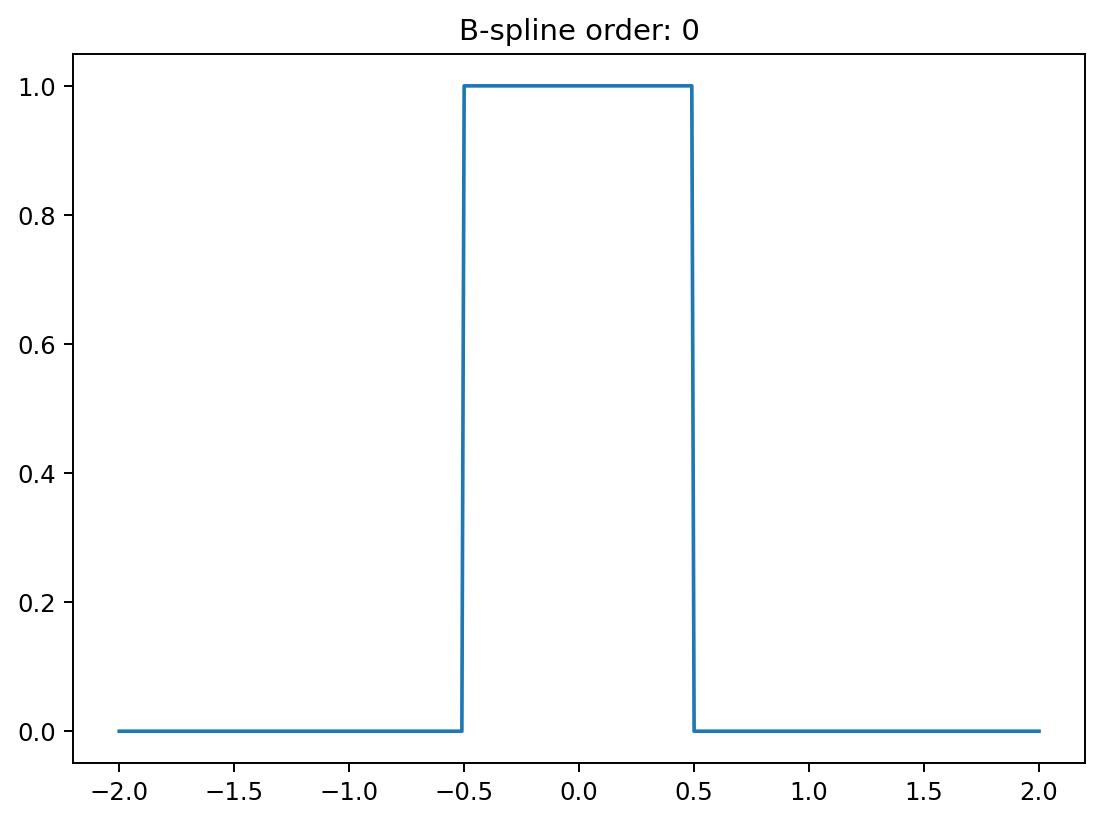
\includegraphics[width=0.3\textwidth]{BSpline_order0}
  \hfill
  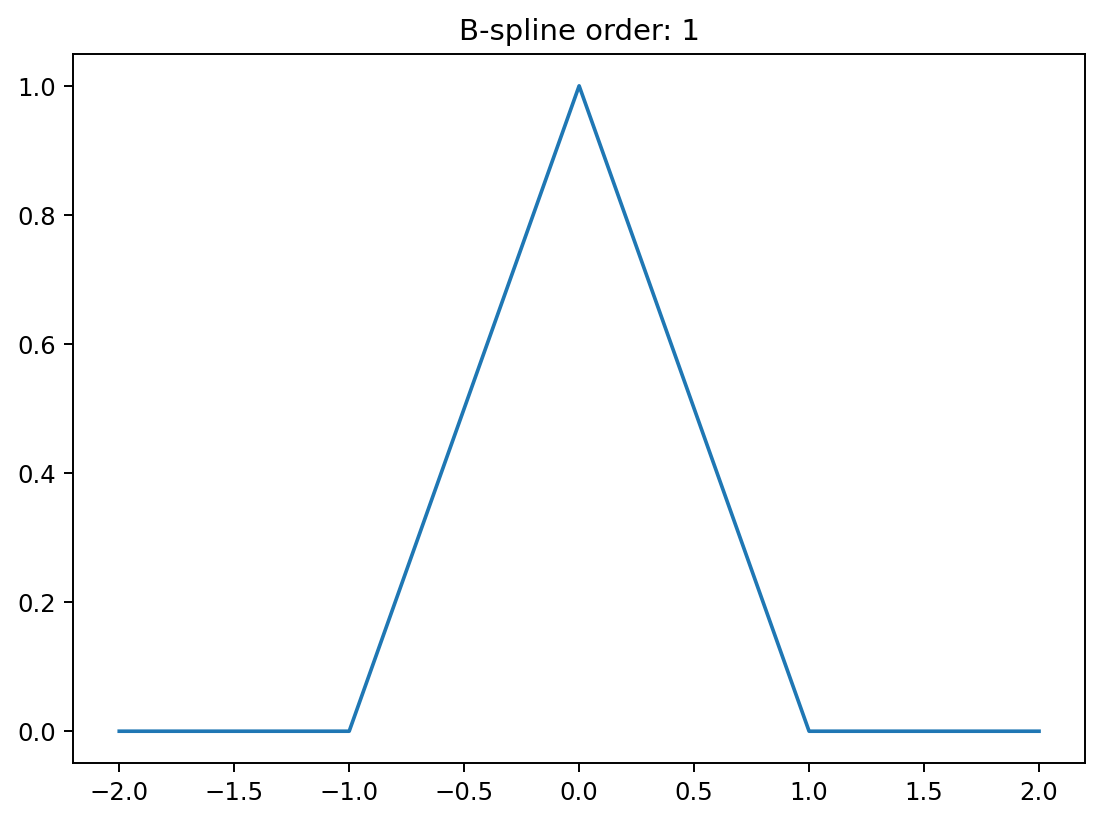
\includegraphics[width=0.3\textwidth]{BSpline_order1}
  \hfill
  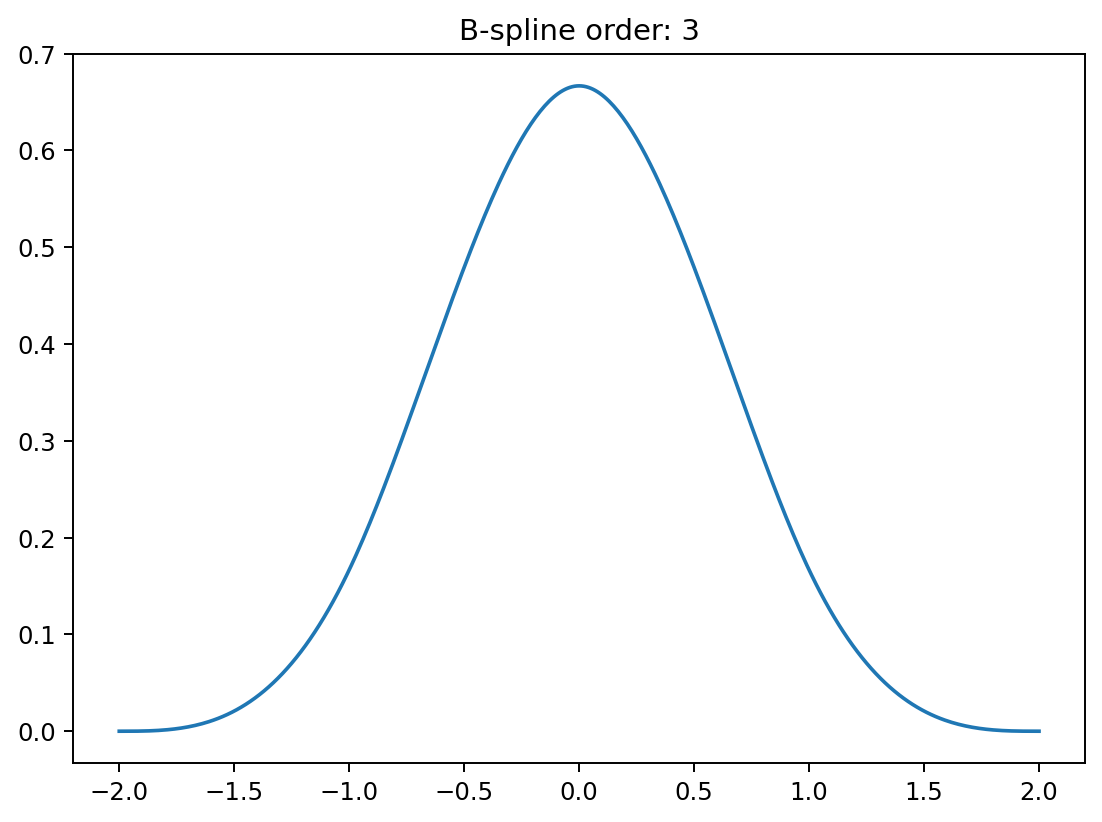
\includegraphics[width=0.3\textwidth]{BSpline_order3}
  \caption{B-splines $\beta^0( x )$, $\beta^1( x )$ and $\beta^3( x )$.}
  \label{fig:Bsplines}
\end{figure}


B-splines are typically used to construct basis functions by scaling them with some factor $h$, and shifting them to be $h$ unites apart:
% %
% \footnote{
% The usefulness of these type of basis functions stems from their limited support (they are only non-zero within a small range), limiting the number of terms that need to be computed when evaluating~\eqref{eq:prediction1D} to just a few,
% as well as favorable numerical 
% (the required matrix inversions can be performed with very fast filter-based methods)
% and analytical properties in interpolation applications~\cite{UnserXXX}.
% ).}%
% :
\begin{equation}
\phi_m(x) = \beta^p \left( \frac{x - m h}{h} \right).
\label{eq:BsplineBasisFunction}
\end{equation}
%
This is illustrated in Fig.~\ref{fig:basisFunctions1D_BSpline} for the case $h=25$.
%
The usefulness of these type of basis functions stems from their limited support (they are only non-zero within a small range), which can be used to dramatically reduce the number of terms that need to be summed over 
% making predictions
in practical implementations (e.g., in~\eqref{eq:prediction1D}).
Furthermore, in interpolation applications B-splines enjoy a number of theoretical and numerical advantages (e.g., the curvature of $y( x, \fat{w} )$ is minimized, and the required matrix inversions can be performed with very fast filter-based methods)~\cite{UnserSPM1999}.


\subsection{Smoothing}

In some applications, the measurements 
% $\fat{t}$ 
% $\{t_n\}_{n=1}^N$
$t_n, n=1,\ldots,N$
are only noisy observations, 
and the aim is to recover the ``denoised'' underlying signal $\hat{t}_n = y( x_n, \fat{w} )$ at the locations $x_n$.
%
Collecting these denoised estimates into a vector
$\fat{\hat{t}} = (\hat{t}_1, \ldots, \hat{t}_N)\transp$,
we obtain (cf.~\eqref{eq:prediction1D}):
\begin{equation}
\fat{\hat{t}} = \bldgr{\Phi} \fat{w}
.
\label{eq:smoothingExpansion}
\end{equation}
Plugging in the solution~\eqref{eq:coefficientsWithRegularization} then yields
% $$
% \fat{\hat{t}} 
% = 
% \bldgr{\Phi} 
% \left( \bldgr{\Phi}\transp \bldgr{\Phi} + \lambda \bldgr{\Omega}\transp \bldgr{\Omega} \right)^{-1}
% \bldgr{\Phi}\transp \fat{t}
% $$
$$
\fat{\hat{t}} 
= 
\fat{S} \fat{t},
$$
where
$$
\fat{S} = 
\bldgr{\Phi} 
\left( \bldgr{\Phi}\transp \bldgr{\Phi} + \lambda \bldgr{\Omega}\transp \bldgr{\Omega} \right)^{-1}
\bldgr{\Phi}\transp
$$
is a $N \times N$ ``smoothing'' matrix that transforms a noisy signal $\fat{t}$ into a ``denoised'' signal $\fat{\hat{t}}$ by making linear combinations of the elements in $\fat{t}$. The $n$-th row of $\fat{S}$ contains the weights assigned to the various elements of $\fat{t}$ in the computation of $\hat{t}_n$, as illustrated in Fig.~\ref{fig:smoothing1D} (bottom row).

The amount of smoothing that is applied can be controlled by both the number of basis functions $M$ and the regularization parameter $\lambda$: choosing higher $M$ or lower $\lambda$ will produce less smoothing. 
This effect is illustrated in Fig.~\ref{fig:smoothing1D}.
In the limit, when $M = N$ and $\lambda = 0$, $\fat{S}$ becomes the identify matrix%
\footnote{Because $\bldgr{\Phi}$ is square when $M=N$, so that $( \bldgr{\Phi}\transp \bldgr{\Phi} )^{-1} = \bldgr{\Phi}^{-1} (\bldgr{\Phi}\transp)^{-1}$.}
and no smoothing is applied at all.  

\begin{figure}
  \centering
  \begin{subfigure}{0.32\textwidth}
     \centering
     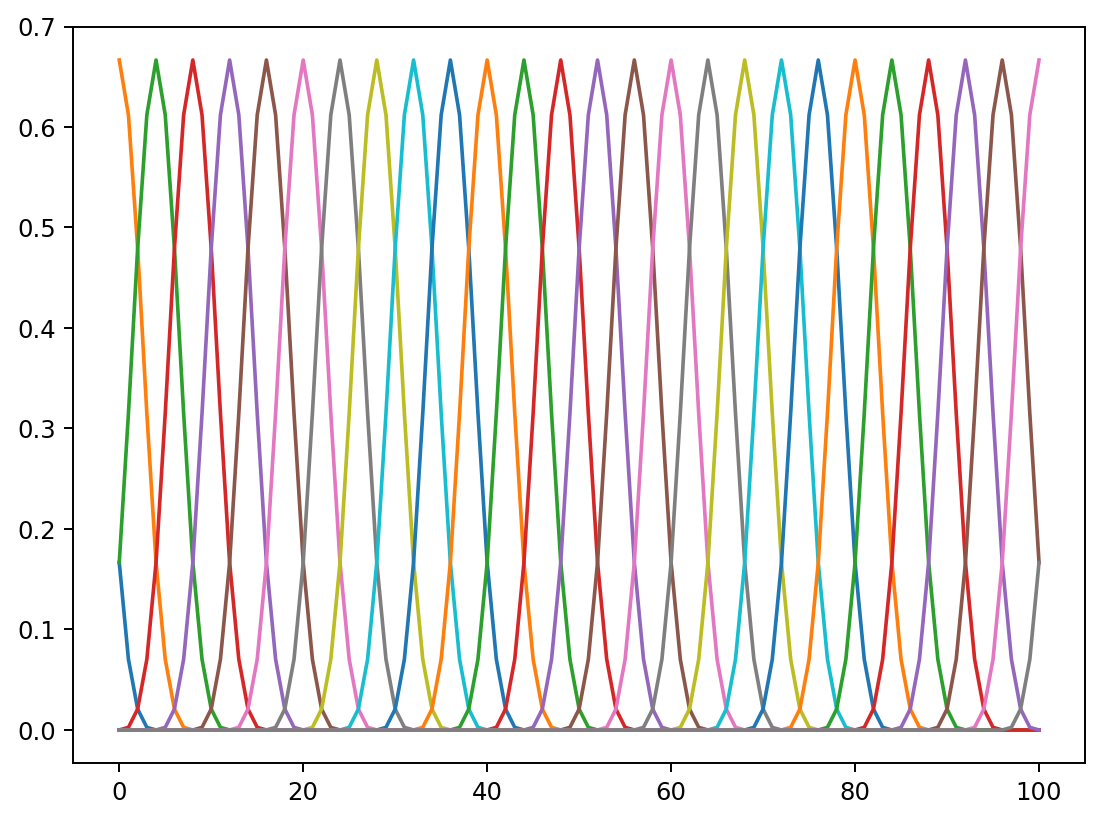
\includegraphics[width=\textwidth]{smoothing_M28_gamma0_basisFunctions}
     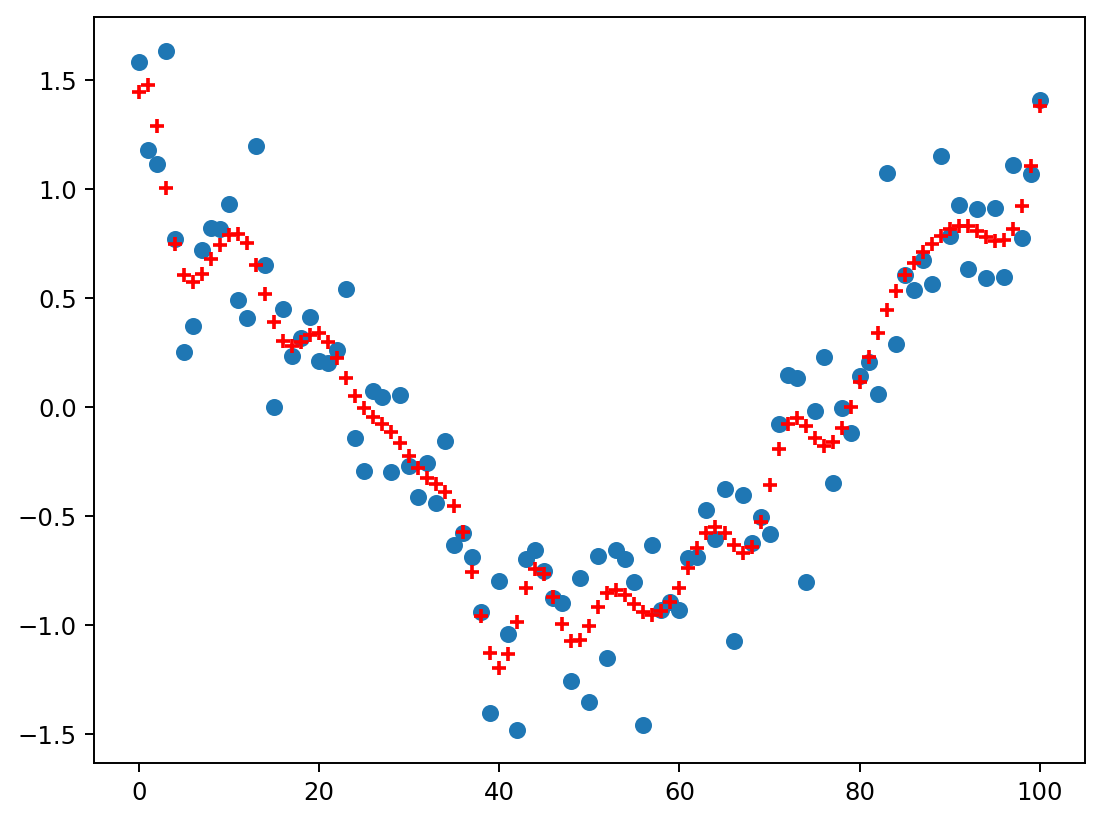
\includegraphics[width=\textwidth]{smoothing_M28_gamma0_fitted}
     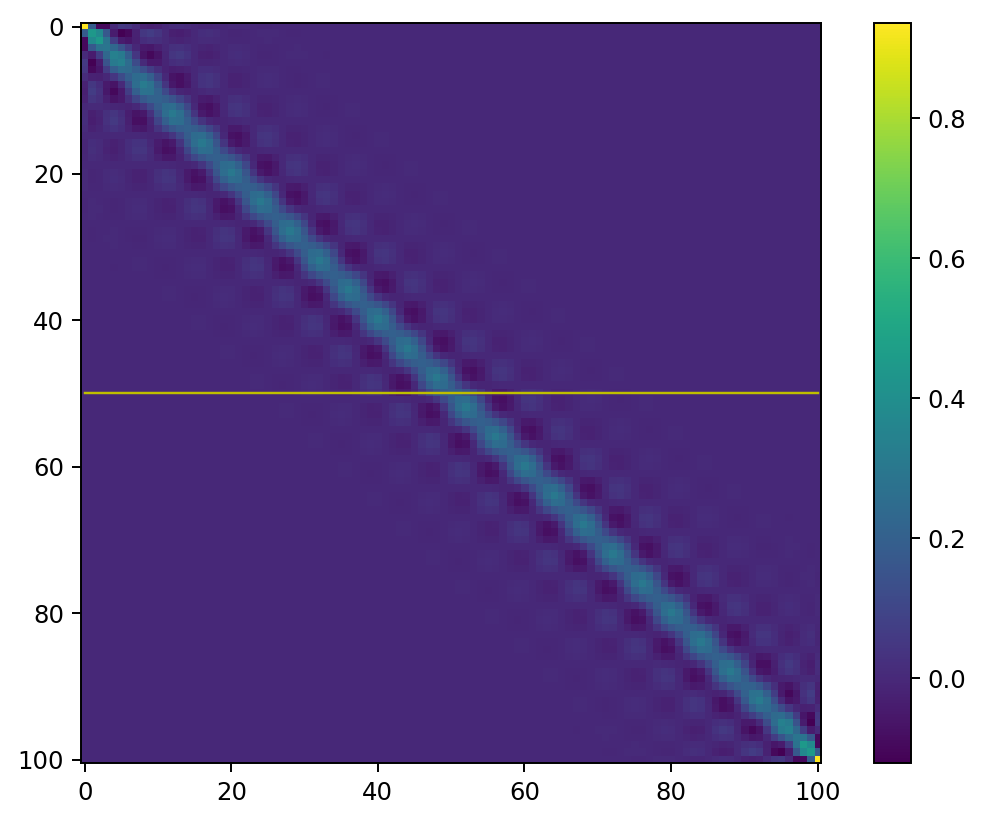
\includegraphics[width=\textwidth]{smoothing_M28_gamma0_smoothingMatrix}
     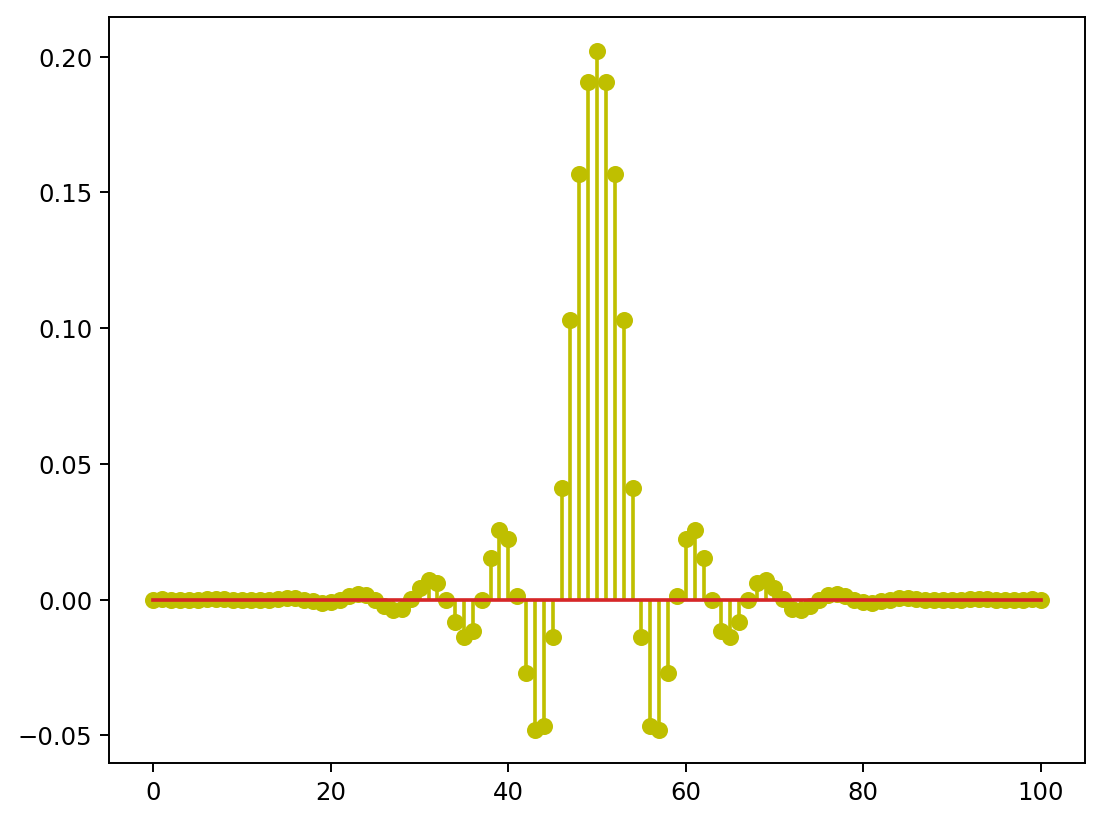
\includegraphics[width=\textwidth]{smoothing_M28_gamma0_smoothingKernel}
     \caption{$M=28$ and $\gamma=0$}
     \label{fig:smoothing_M28_gamma0}
  \end{subfigure}
  \hfill
  \begin{subfigure}{0.32\textwidth}
     \centering
     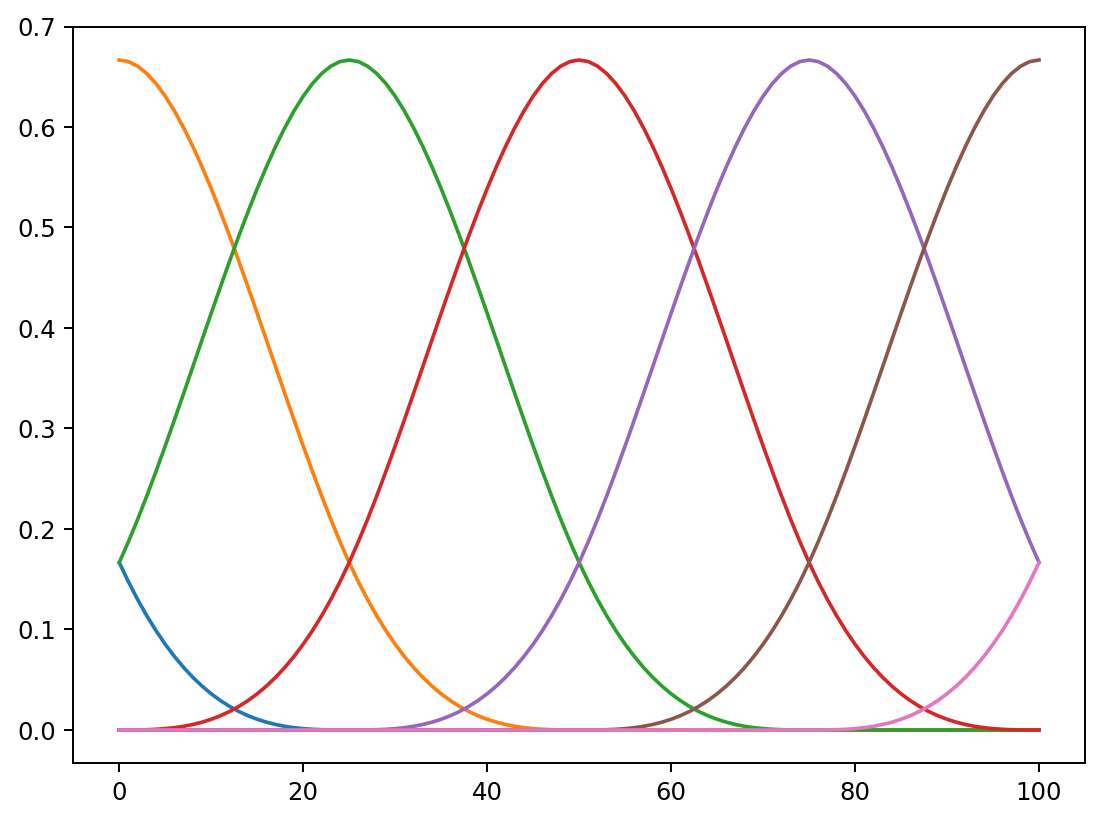
\includegraphics[width=\textwidth]{smoothing_M7_gamma0_basisFunctions}
     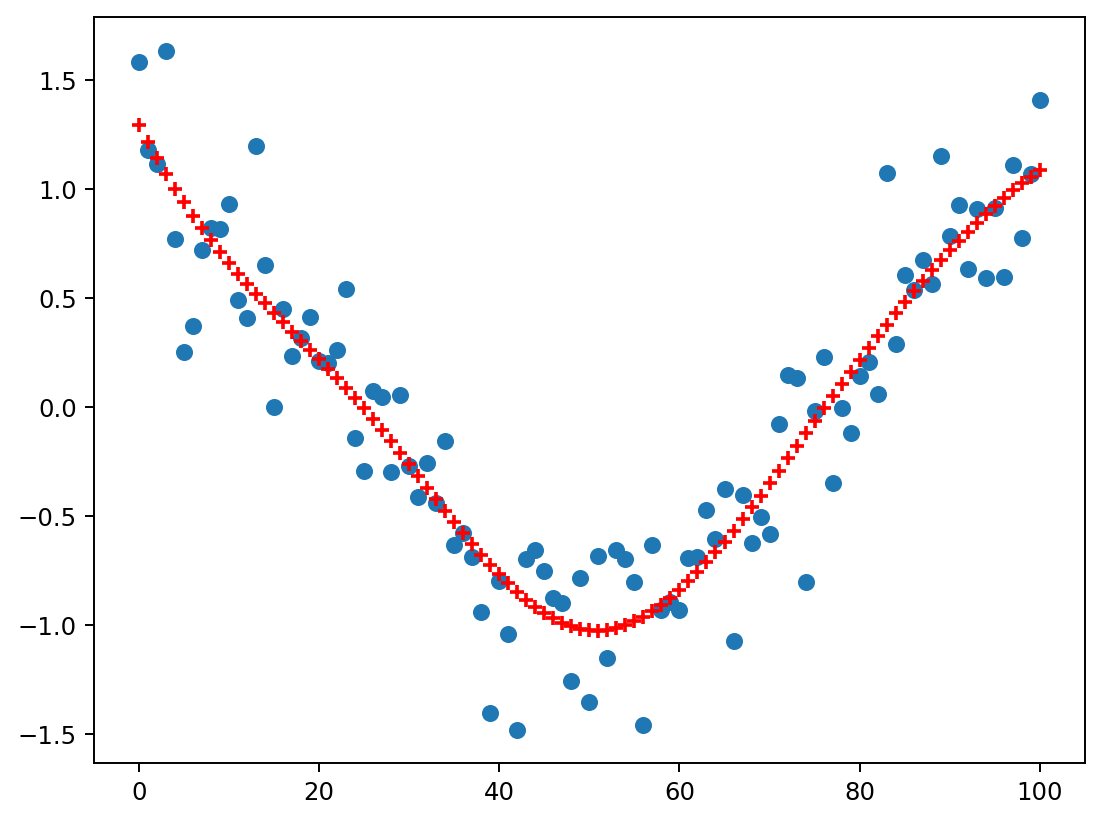
\includegraphics[width=\textwidth]{smoothing_M7_gamma0_fitted}
     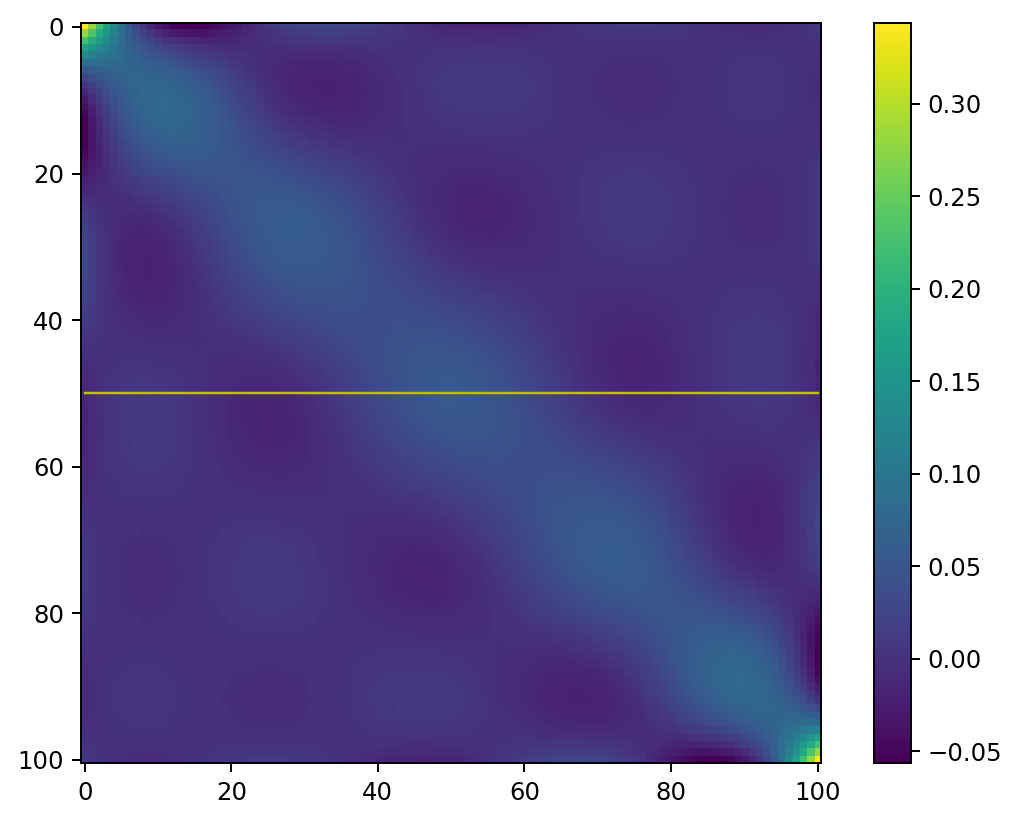
\includegraphics[width=\textwidth]{smoothing_M7_gamma0_smoothingMatrix}
     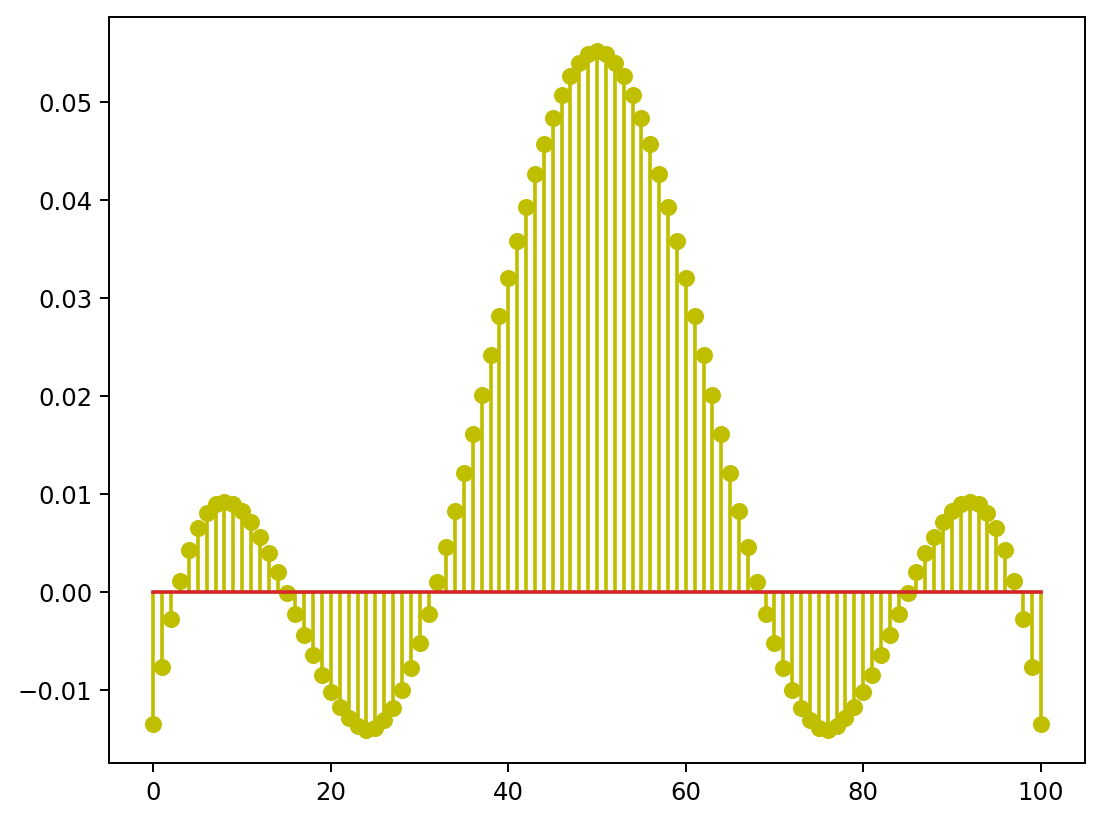
\includegraphics[width=\textwidth]{smoothing_M7_gamma0_smoothingKernel}
     \caption{$M=7$ and $\gamma=0$}
     \label{fig:smoothing_M7_gamma0}
  \end{subfigure}
  \hfill
  \begin{subfigure}{0.32\textwidth}
     \centering
     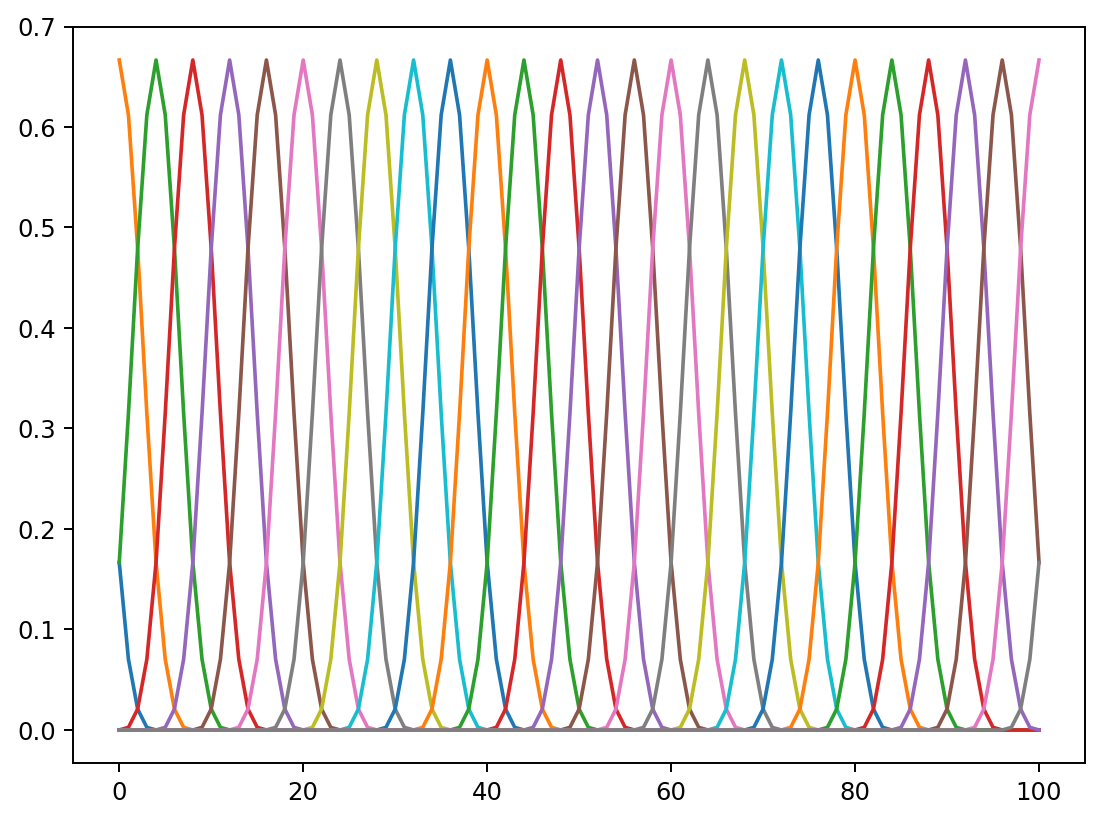
\includegraphics[width=\textwidth]{smoothing_M28_gamma1000_basisFunctions}
     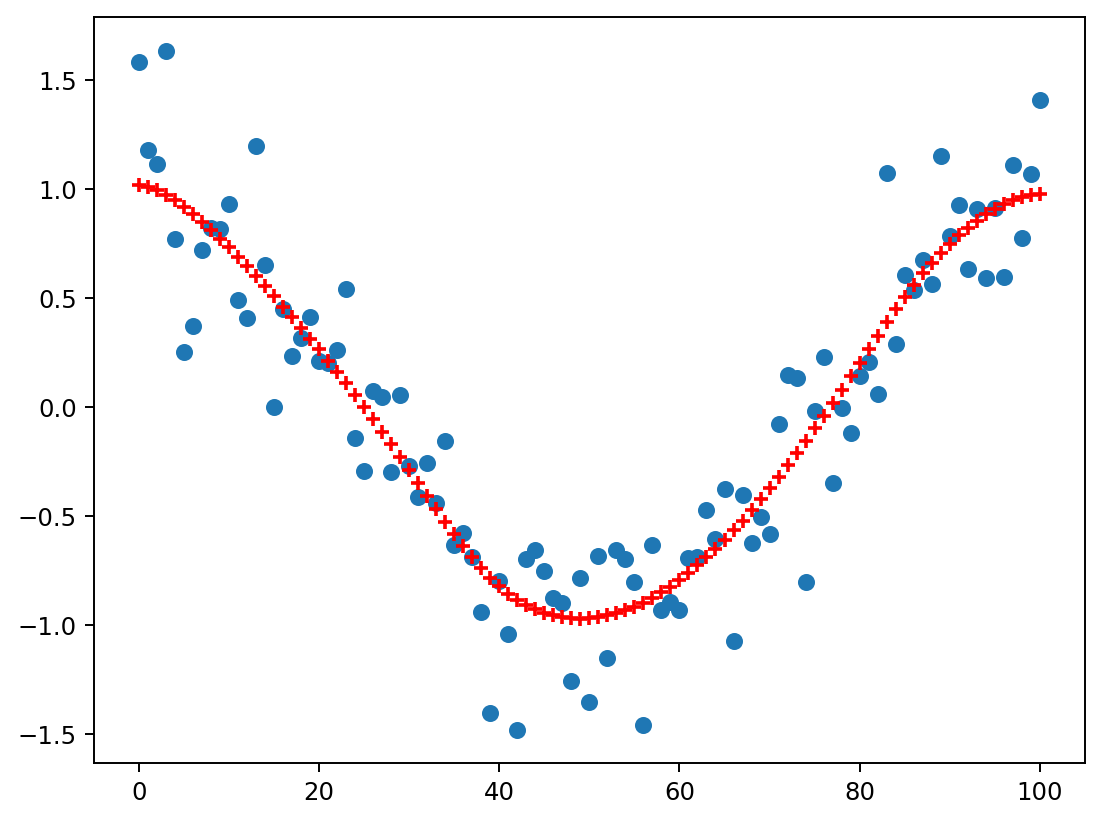
\includegraphics[width=\textwidth]{smoothing_M28_gamma1000_fitted}
     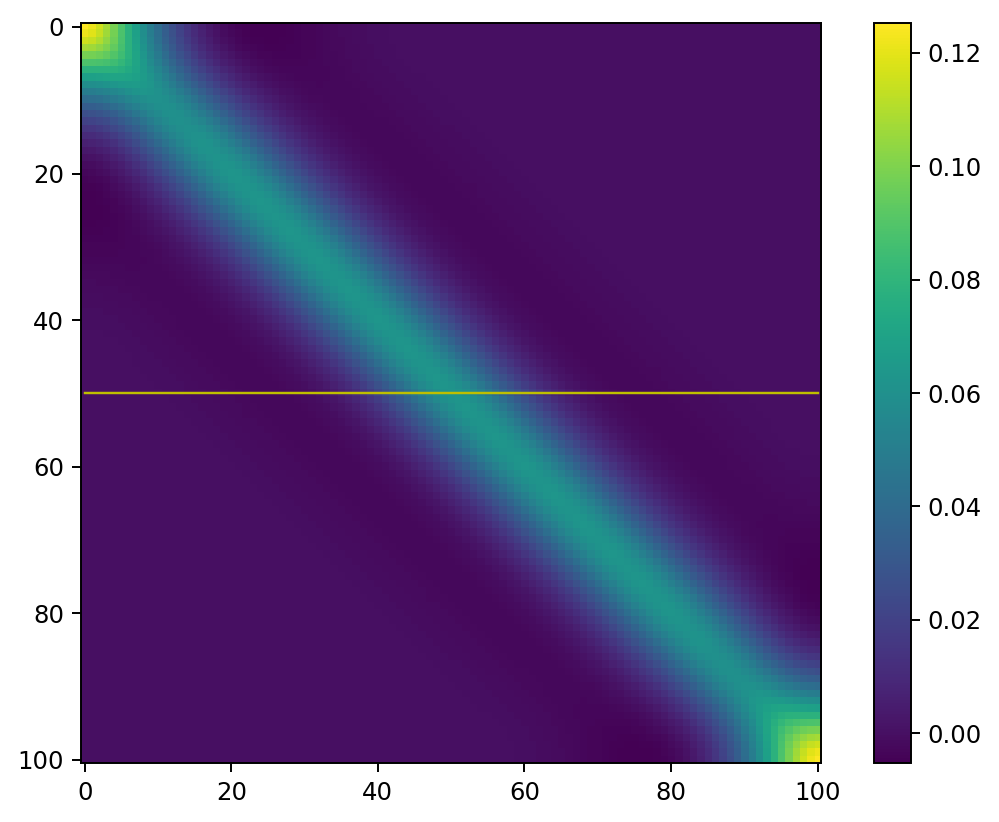
\includegraphics[width=\textwidth]{smoothing_M28_gamma1000_smoothingMatrix}
     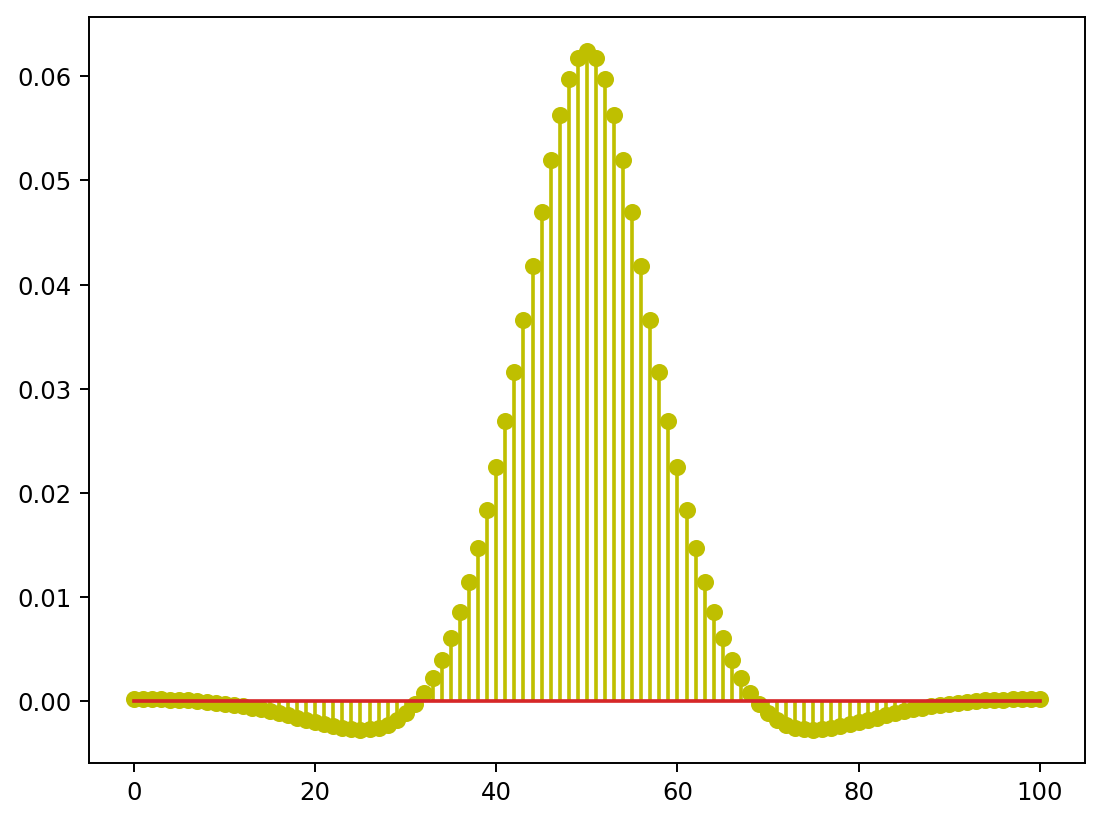
\includegraphics[width=\textwidth]{smoothing_M28_gamma1000_smoothingKernel}
     \caption{$M=28$ and $\gamma=1000$}
     \label{fig:smoothing_M28_gamma1000}
  \end{subfigure}
  \caption{Smoothing of a 1D signal when the number of basis functions ($M$) and the regularization strength ($\gamma$) is varied. 
  The regularizer is of the form $\bldgr{\Omega} = \bldgr{\Gamma} \bldgr{\Phi}$, where $\bldgr{\Gamma}$ computes second-order finite differences (the $n$-th row has all zeros except for columns $n-1$, $n$ and $n+1$, who have elements -1, 2 and -1, respectively). From top to bottom: basis functions that were used; noisy signal $\fat{t}$ and denoised signal $\fat{\hat{t}}$ in blue and red, respectively; smoothing matrix $\fat{S}$; and the middle row of $\fat{S}$.
  }
  \label{fig:smoothing1D}
\end{figure}




\newcounter{myFootnoteValueSaver}
\setcounter{myFootnoteValueSaver}{\value{footnote}}


\subsection{Interpolation}

When several medical images need to be compared, a common problem is that the intensities of an image need to be evaluated at locations $x$ different from the integer locations $x_1\!=\!0, x_2\!=\!1, \ldots x_N\!=\!N\!-\!1$ where the intensities $t_1, t_2, \ldots, t_N$ are defined.  
%
A standard solution is to 
set $\lambda=0$, and
use the shifted B-spline basis functions of~\eqref{eq:BsplineBasisFunction} with scaling factor $h=1$, i.e., a B-spline $\beta^p$ is centered around each of the $N$ integer coordinates $x_n$.
%
Because $M=N$, the solution is given by%
\footnotemark[\value{myFootnoteValueSaver}]
$$
\fat{w} = \bldgr{\Phi}^{-1} \fat{t}
,
$$
for which fast, dedicated numerical solvers are available~\cite{UnserSPM1999}.

As already analyzed above, the resulting function $y(x, \fat{w})$ will pass exactly through the original intensities $t_n$ at the integer locations $x_n$.
However, the model will also fill in ``interpolating'' intensity values everywhere else, with the exact behavior depending on the order of the B-spline. For order $p=0$, so-called \emph{nearest neighbor} interpolation is obtained, in which the predicted value at location $x$ is simply the value $t_n$ of the measurement location $x_n$ that is nearest to $x$%
\footnote{Strictly speaking an exception is made at locations $x$ that fall exactly half-way between two integer locations,
% $x_n$ and $x_{n+1}$, where the value $(t_n + t_{n+1})/2$ is returned.
where the average value is returned.
}
.
For $p=1$, \emph{linear} interpolation is obtained, in which $y(x, \fat{w})$ is piece-wise linear between the 
% measurement sites 
integer locations
$\{x_n\}_{n=1}^N$.
%
Finally, $p=3$ results in so-called \emph{cubic} interpolation, which is the method of choice in most practical applications.
The effect of the B-spline order on the interpolation behavior of the model is illustrated in Fig.~\ref{fig:interpolation1D}.


\begin{figure}
  \centering
  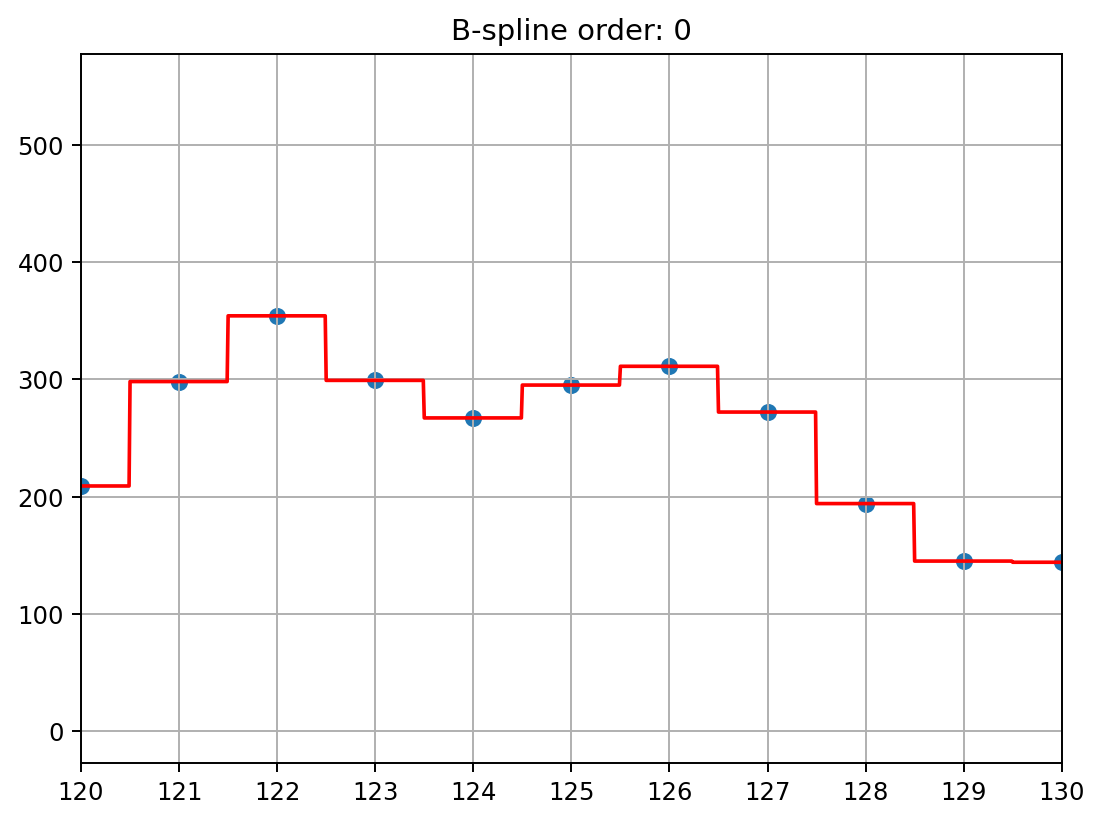
\includegraphics[width=0.48\textwidth]{interpolation_BSplineOrder0}
  \hfill
  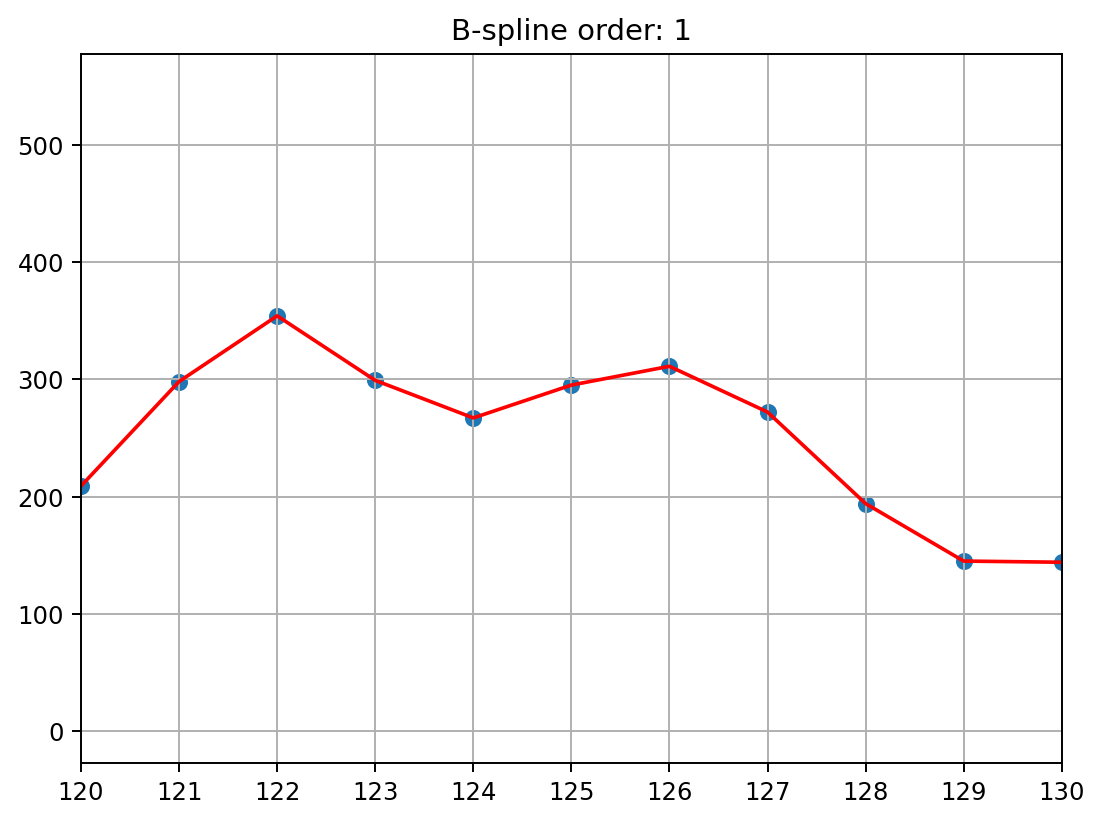
\includegraphics[width=0.48\textwidth]{interpolation_BSplineOrder1}
  \hfill
  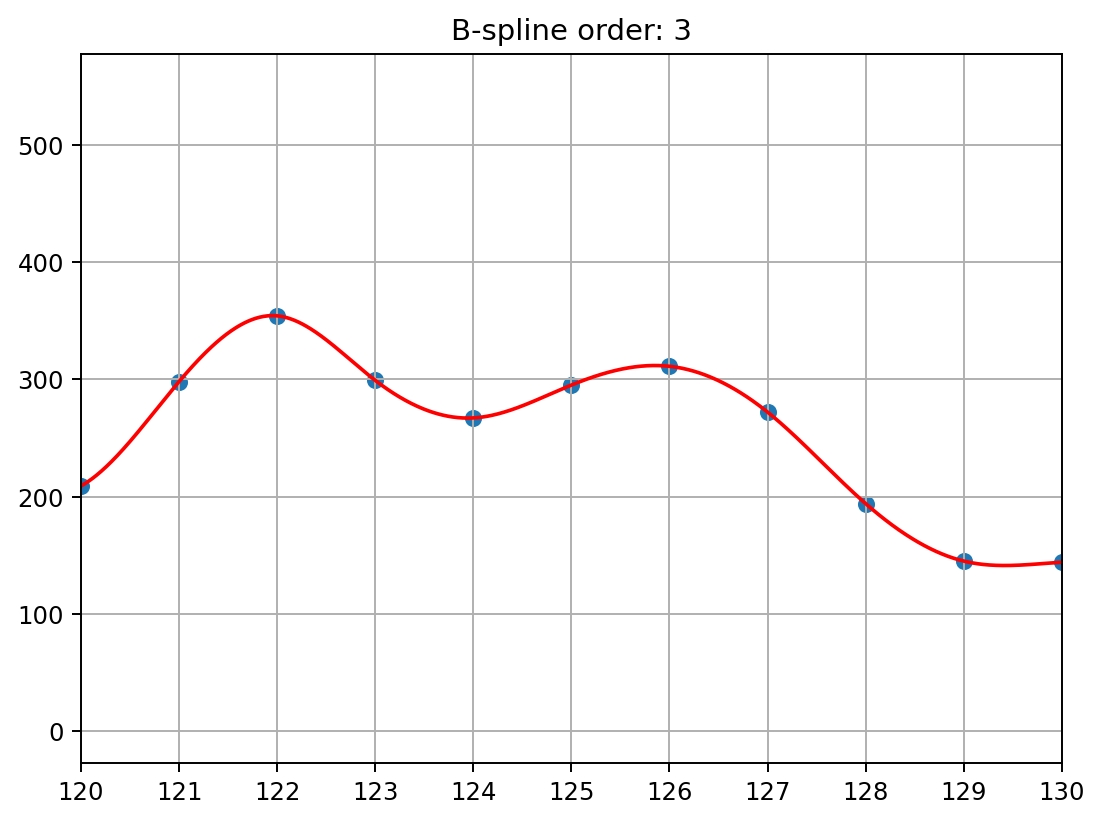
\includegraphics[width=0.48\textwidth]{interpolation_BSplineOrder3}
  \caption{Nearest-neighbor, linear and cubic interpolation.}
  \label{fig:interpolation1D}
\end{figure}



\section{Smoothing and interpolation in higher dimensions}
\label{sec:smoothingAndInterpolationND}

When going to $D=2$ dimensions, the spatial locations $\fat{x} = (x_1, x_2)$ consist of two coordinates $x_1$ and $x_2$, and the measurement signal becomes a two-dimensional image, represented by a matrix with $N_1$ rows and $N_2$ columns:
$$
\fat{T} = 
\left(
\begin{array}{cccc}
t_{1,1} & t_{1,2} & \cdots & t_{1,N_2} \\ 
t_{2,1} & t_{2,2} & \cdots & t_{2,N_2} \\ 
\vdots & \vdots & \ddots & \vdots \\ 
t_{N_1,1} & t_{N_1,2} & \cdots & t_{N_1,N_2} \\ 
\end{array}
\right)
.
$$
% where the rows correspond 
It will be convenient to define a \emph{vectorization} 
operation 
-- denoted by $\mathrm{vec}(\cdot)$ --
that re-arranges this $N_1 \times N_2$ image into a 1D signal $\fat{t}$ of length $N = N_1 N_2$, by stacking the columns of $\fat{T}$ under each other:
\begin{equation}
\fat{t} = 
\mathrm{vec}( \fat{T} )
=
\left(
\begin{array}{c}
t_{1,1} \\
\vdots \\
t_{N_1,1} \\
t_{1,2} \\
\vdots \\
t_{N_1,2} \\
\vdots \\
t_{N_1,N_2}
\end{array}
\right)
.
\label{eq:vec}
\end{equation}
In this re-arrangement, element $t_{{n_1},{n_2}}$ in $\fat{T}$ corresponds to element $t_n$ in $\fat{t}$, where $n = n_1 + (n_2-1) N_1$.

%
In order to proceed, we also need to choose appropriate basis functions 
$\phi_m(\fat{x})$ that work in 2D. A convenient choice is often \emph{separable} basis functions, which are simply the product of two 1D basis functions (one taking as input $x_1$, and the other one $x_2$). If there are $M_1$ basis functions in the first (row) direction, and $M_2$ in the second (column) direction, 
taking all the combinations yields 
a total of $M = M_1 M_2$ basis functions in 2D, given by
\begin{equation}
\phi_m( \fat{x} ) = \phi_{m_1}( x_1 ) \phi_{m_2}( x_2 ) 
\label{eq:basisFunction2D}
\end{equation}
for $m = m_1 + m_2 M_1$ (recall that $m_1$ and $m_2$ run from $0$ to $M_1-1$ and $M_2-1$ respectively).
%
Fig.~\ref{fig:basisFunctions2D_BSpline} illustrates the 2D basis functions generated from 1D 
% DCT and 
B-spline basis functions this way.

\begin{figure}
  \centering
  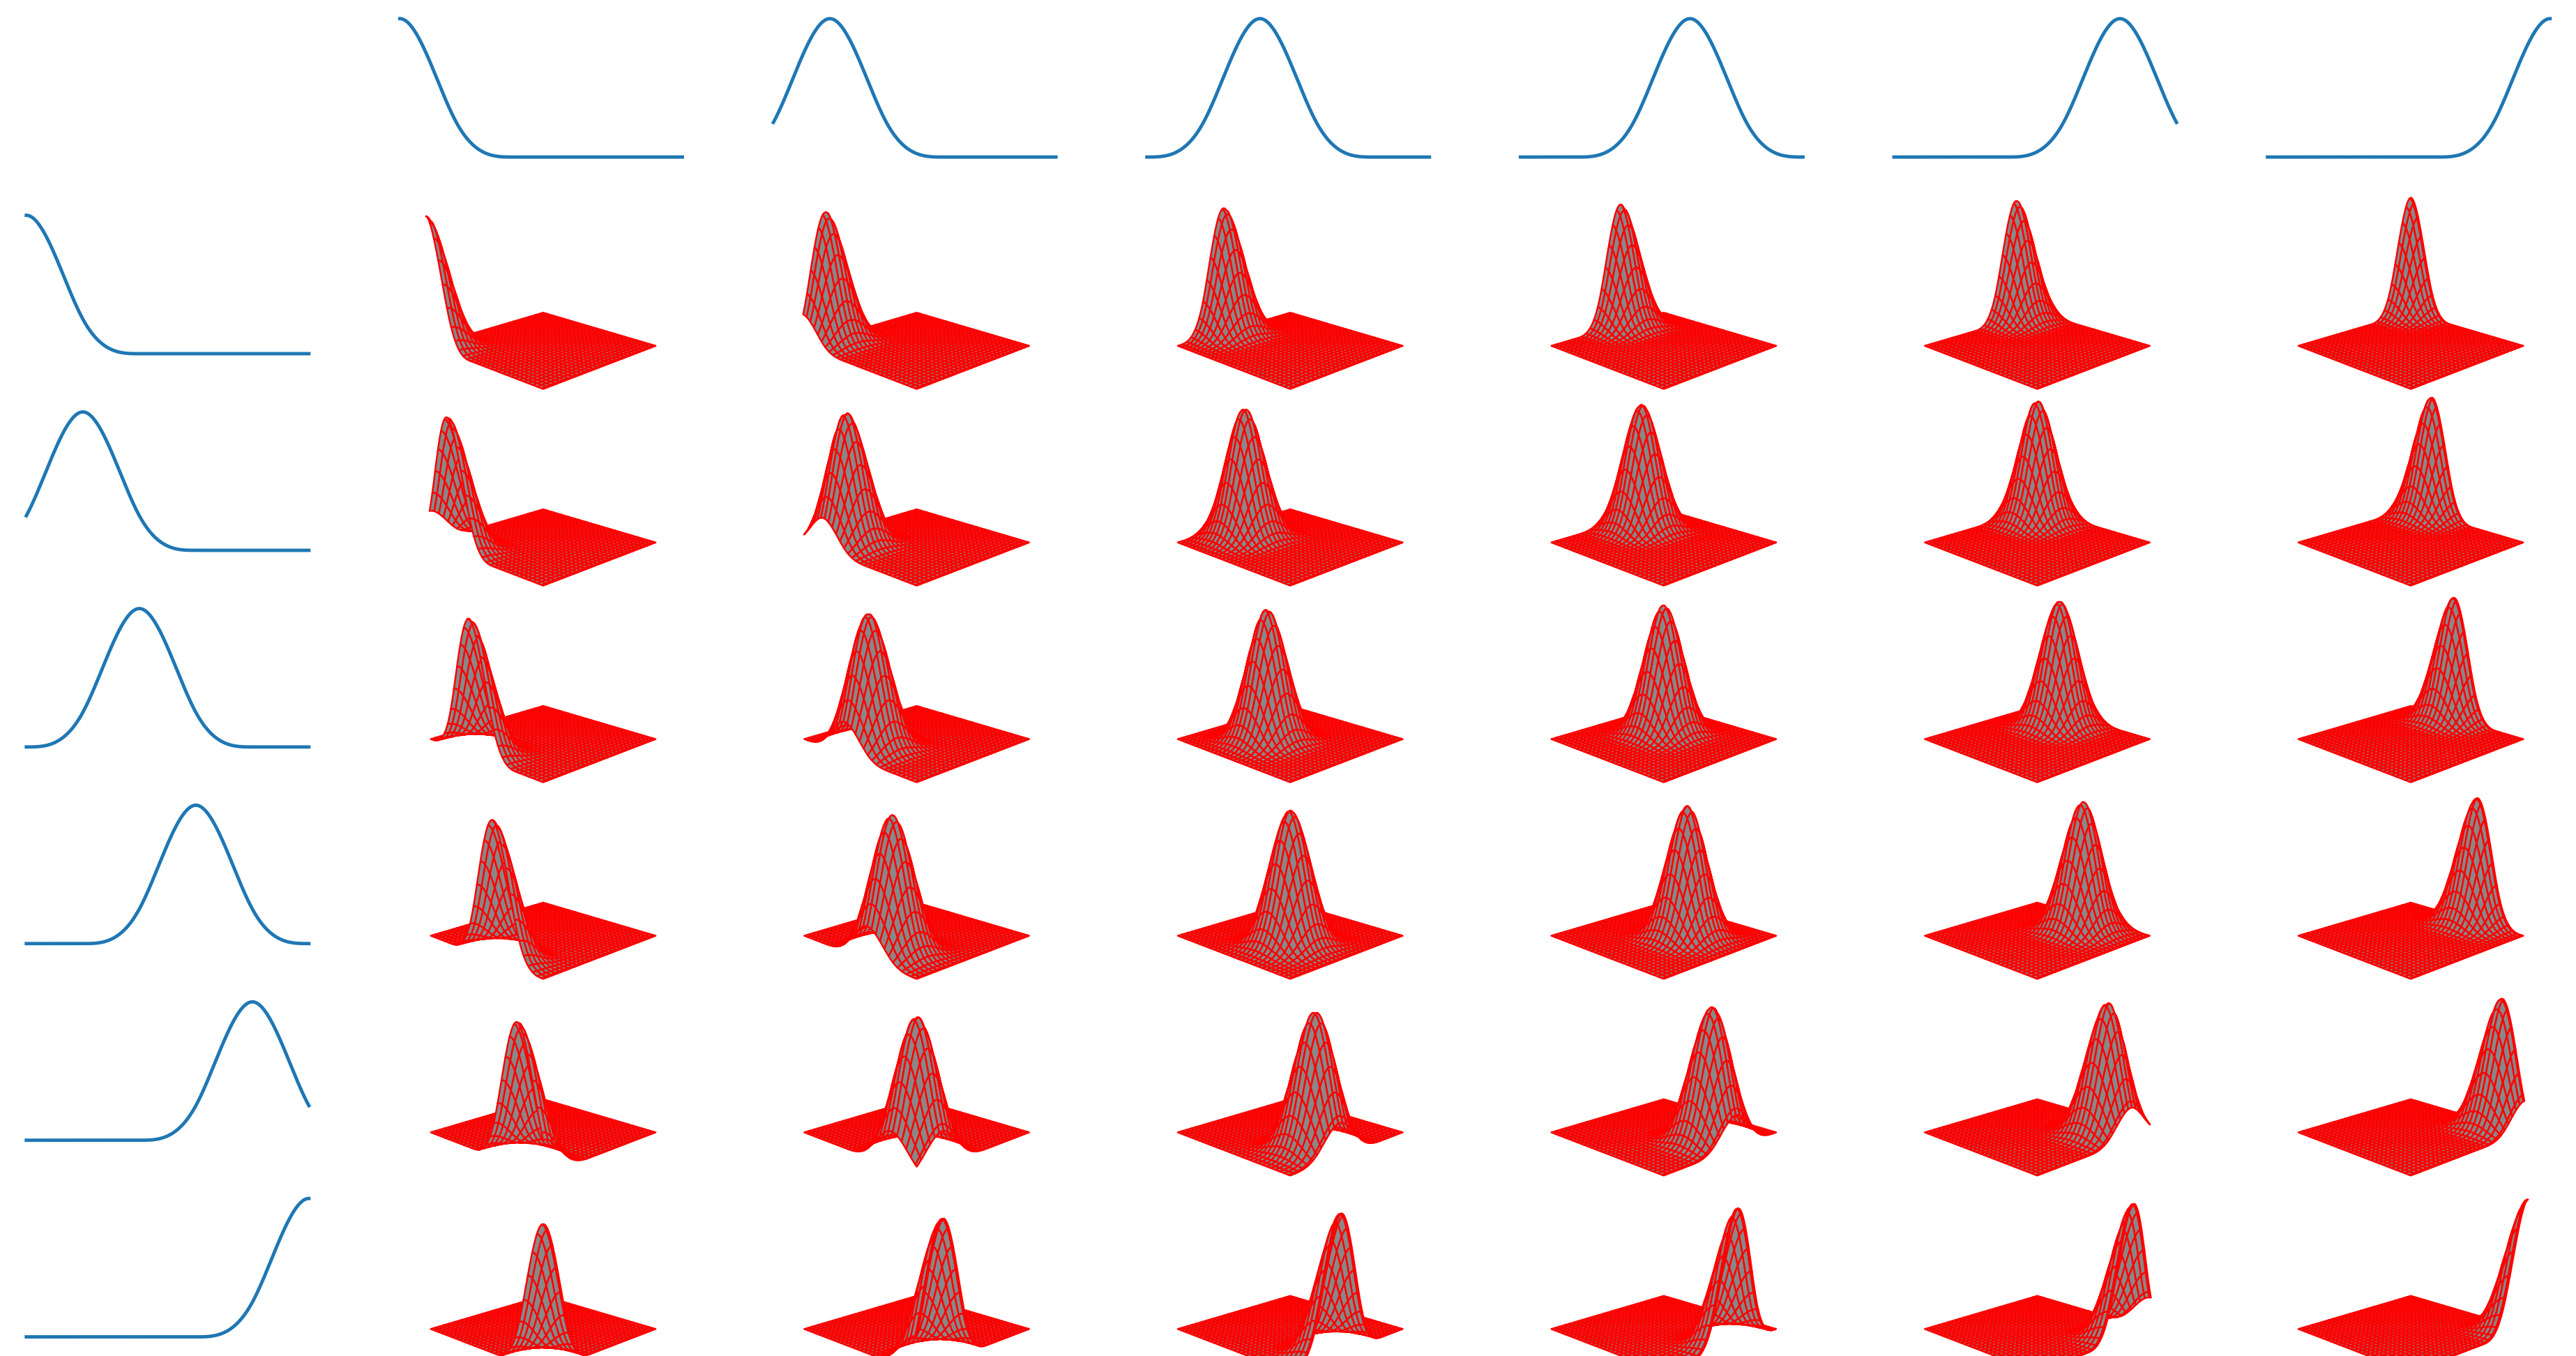
\includegraphics[width=\textwidth]{smoothing2D_decimationFactor51_basisFunctions}
  %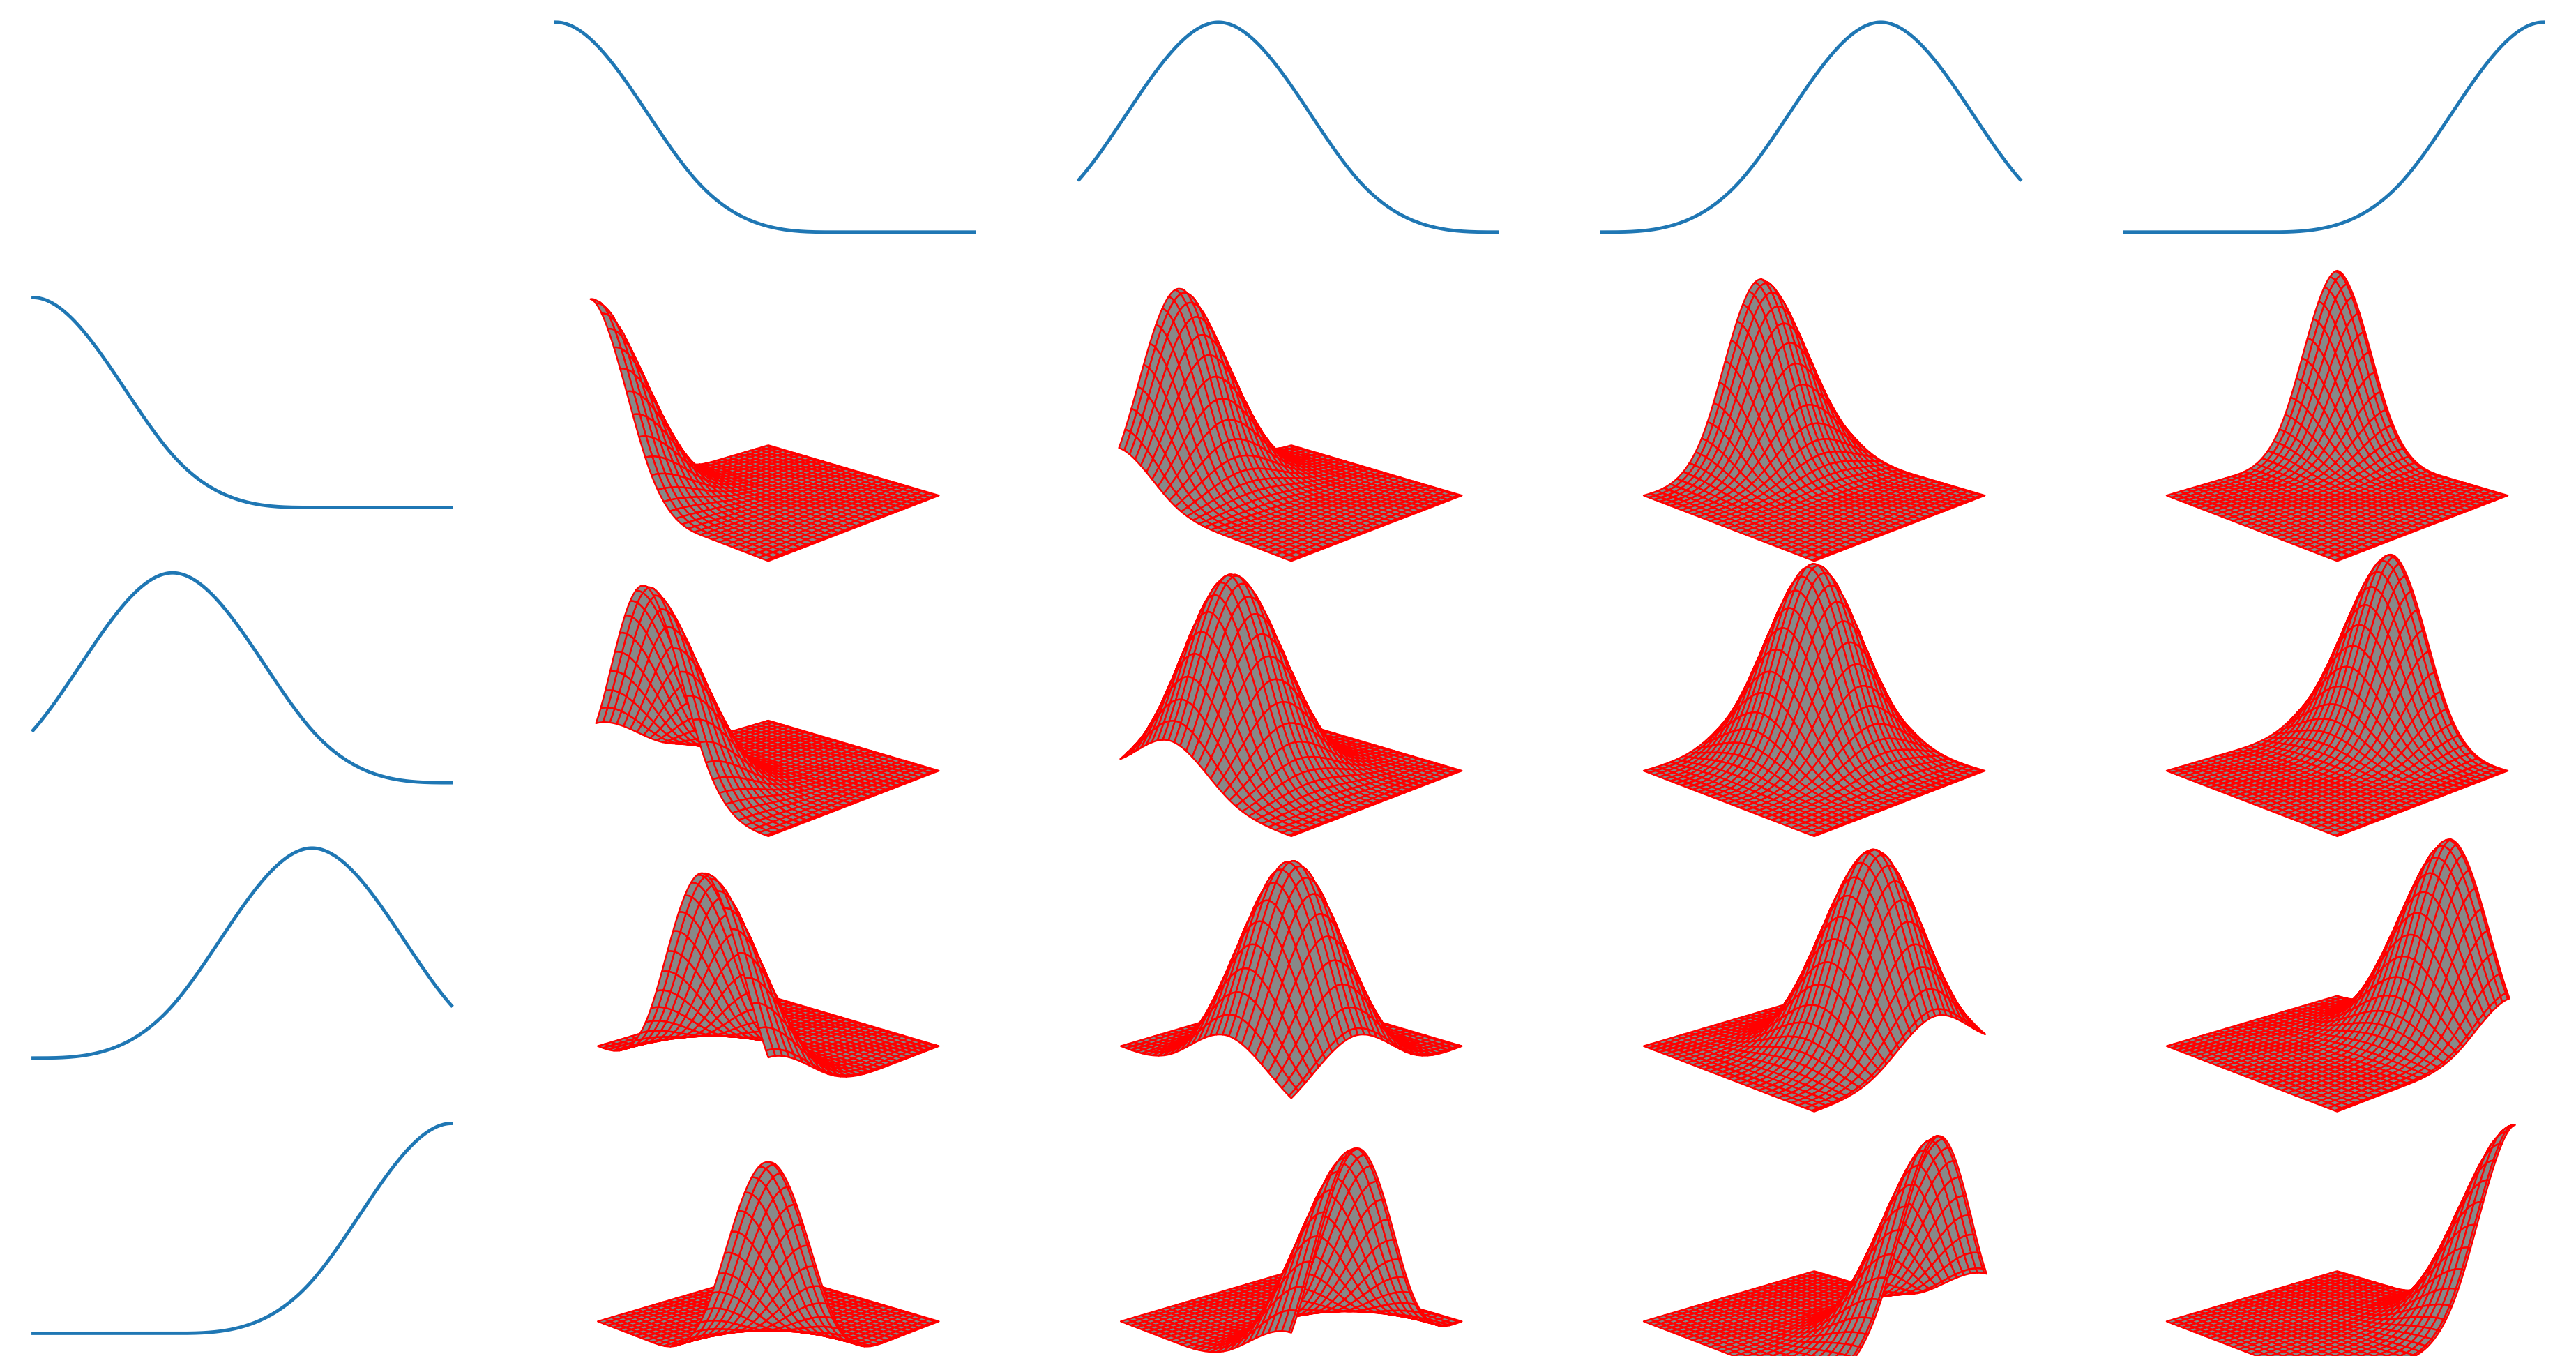
\includegraphics[width=\textwidth]{smoothing2D_decimationFactor85_basisFunctions}
  \caption{The 36 separable 2D basis functions produced from two sets of 6 1D basis functions.}
  \label{fig:basisFunctions2D_BSpline}
\end{figure}


%
To simplify notation, it will be convenient to use the Kronecker product of two matrices:
$$
\fat{A} \otimes \fat{B} =
\left(
\begin{array}{c|c|c}
a_{1,1} \fat{B} & a_{2,1} \fat{B} & \hdots \\
\hline
a_{2,1} \fat{B} & a_{2,2} \fat{B} & \hdots \\
\hline
\vdots          & \vdots          & \ddots
\end{array}
\right)
.
$$
%
If $\bldgr{\Phi}_1$ denotes the $N_1 \times M_1$ matrix containing the output of the $M_1$ basis functions evaluated at the integer locations $x_1=0,\ldots,N_1-1$, and $\bldgr{\Phi}_2$ is similarly defined for the second direction, then 
\begin{equation}
\bldgr{\Phi} = \bldgr{\Phi}_2 \otimes \bldgr{\Phi}_1
\label{eq:Phi2D}
\end{equation}
is a $N \times M$ matrix that contains vectorized versions of all $M$ basis functions in 2D, where the $m$-th column contains~\eqref{eq:basisFunction2D} evaluated at all the pixel locations in $\fat{T}$.

%
Equipped with~\eqref{eq:vec},~\eqref{eq:basisFunction2D} and~\eqref{eq:Phi2D}, any smoothing or interpolation problem in 2D can be directly mapped into a 1D problem,
so that the solutions described in Sec.~\ref{sec:smoothingAndInterpolation1D} can (in principle) be directly applied. 
%
The extension to 3D is also straightforward; for example, vectorized versions of the output of $M = M_1 M_2 M_3$ basis functions, evaluated at all $N = N_1 N_2 N_3$ locations, are given by
$$
\bldgr{\Phi} = \bldgr{\Phi}_3 \otimes \bldgr{\Phi}_2 \otimes \bldgr{\Phi}_1 
.
$$


\subsection{Exploiting separability}

Although the problem is in theory solved, in practice the computations involve storing and inverting a $M \times M$ matrix, which can be problematic when $M$ is very large (i.e., when the model involves many basis functions). As an example, consider the interpolation of a 3D volume of size $256 \times 256 \times 256$, an application in which there are $M = 256^3$ basis functions. At this size, naively storing a matrix with $M^2$ elements at 64 bits per element (double-precision floating point) would take 
% (256^3)^2 * 8 = (2^8)^6 * 2^3 = 2^51 bytes
% 2^51 / 2^30 = 2^21 GB = 2097152 GB
% 2^51 / 2^40 = 2^11 TB = 2048 TB
2048 TB; subsequently inverting it would take 
%$\mathcal{O}( M^3 )$ 
$\mathcal{O}( M^3 ) = \mathcal{O}( 256^9 )$ 
operations, making it entirely infeasible. 
In contrast, re-arranging the computations as outlined below only requires storing and inverting three $256 \times 256$ matrices, taking 
% 256^2 * 8 = (2^8)^2 * 2^3 = 2^19 bytes
% 2^19 / 2^10 = 2^9 = 512 KB
512 KB and 
$\mathcal{O}( 256^3 )$ operations each.
%
For a 2D image of size $256 \times 256$, the savings are more modest but still very substantial:
% (256^2)^2 * 8 = (2^8)^4 * 2^3 = 2^35 bytes
% 2^35 / 2^20 = 2^15 = 32768 MB
% 2^35 / 2^30 = 2^5 = 32 GB
storing a matrix of 32 GB vs.~two matrices of 
% (256^2) * 8 = (2^8)^2 * 2^3 = 2^19 bytes
% 2^19 / 2^10 = 2^9 = 512 KB
512 KB,
and 
$\mathcal{O}( 256^6 )$ operations vs.~two times 
$\mathcal{O}( 256^3 )$ operations for matrix inversions, 
% 256^6 / ( 2 * 256^3 ) = 2^48 / 2^25 = 2^23 = 8,388,608
which is almost 10 million times faster.

When no regularization is used ($\lambda = 0$), 
% where the solution is given by~\eqref{eq:coefficients}, 
the separability of the basis functions can be exploited
as follows.
% .to compute the solution~\eqref{eq:coefficients} very efficiently.
%
%
In 2D, element $m=m_1 + m_2 M_1$ in the length-$M$ vector $\fat{c} = \bldgr{\Phi}\transp \fat{t}$ is given by
\begin{eqnarray*}
c_m 
& = &
\sum_{n=1}^{N} \phi_{n,m} t_n 
\\
& = & 
\sum_{n_1=1}^{N_1}
\sum_{n_2=1}^{N_2}
\phi_{n_1,m_1}^1 
\phi_{n_2,m_2}^2 
t_{n_1,n_2}
\\
& = & 
\sum_{n_1=1}^{N_1}
\phi_{n_1,m_1}^1 
\left(
\sum_{n_2=1}^{N_2}
\phi_{n_2,m_2}^2 
t_{n_1,n_2}
\right)
,
\end{eqnarray*}
where 
% $\phi_{\cdot,\cdot}^p$ denotes the corresponding element in $\bldgr{\Phi}_p, p=1,\ldots,2$.
$\phi_{\cdot,\cdot}^1$ and 
$\phi_{\cdot,\cdot}^2$ denote elements in $\bldgr{\Phi}_1$ and $\bldgr{\Phi}_2$, respectively.
The key insight is that the same summation over the second direction (in parentheses) is needed for each 
% summation over the first direction, 
new $m_1$,
and therefore needs to be computed only once. In matrix form, this can be expressed as 
$$
\fat{C} = \bldgr{\Phi}_1\transp \fat{T} \bldgr{\Phi}_2,
$$
where $\fat{C}$ is a $M_1 \times M_2$ matrix such that $\mathrm{vec}( \fat{C} ) = \fat{c}$.
Similarly, it can be shown that $\bldgr{\Phi} \fat{w}$ can be more efficiently computed as $\bldgr{\Phi}_x \fat{W} \bldgr{\Phi}_y\transp$, with $\mathrm{vec}( \fat{W} ) = \fat{w}$.
Therefore, the solution~\eqref{eq:coefficients}, which can be written as
$$
\bldgr{\Phi}\transp 
\left(
\bldgr{\Phi}
\fat{w}
\right)
=
\bldgr{\Phi}\transp \fat{t}
,
$$
can also be expressed as 
$$
\bldgr{\Phi}_1\transp
\left(
\bldgr{\Phi}_1\fat{W}\bldgr{\Phi}_2\transp 
\right)
\bldgr{\Phi}_2
=
\bldgr{\Phi}_1\transp
\fat{T}
\bldgr{\Phi}_2
,
$$
so that finally 
\begin{equation}
\fat{W} = 
\left( 
\bldgr{\Phi}_1\transp
\bldgr{\Phi}_1
\right)^{-1}
\bldgr{\Phi}_1\transp
\fat{T}
\bldgr{\Phi}_2
\left( 
\bldgr{\Phi}_2\transp
\bldgr{\Phi}_2
\right)^{-1}
\label{eq:solution2D}
\end{equation}
can be used to compute the elements of $\fat{w}$ very efficiently.

% How much gained? 2D and 3D.

\subsection{Smoothing in 2D}

Plugging the solution~\eqref{eq:solution2D} 
in~\eqref{eq:smoothingExpansion}, and using the same approach as above,
it is easy to see that a smoothed image 
%$\fat{\hat{T}}$ 
can be obtained as
$$
\fat{\hat{T}}
= \fat{S}_1 \fat{T} \fat{S}_2\transp, 
$$
where
% $$
% \fat{S}_d = 
% \bldgr{\Phi}_d 
% \left( \bldgr{\Phi}_d\transp \bldgr{\Phi}_d \right)^{-1} 
% \bldgr{\Phi}_d\transp,
% \quad, d=1,2
% .
% $$
$$
\fat{S}_1 = 
\bldgr{\Phi}_1 
\left( \bldgr{\Phi}_1\transp \bldgr{\Phi}_1 \right)^{-1} 
\bldgr{\Phi}_1\transp
$$
is a $N_1 \times N_1$ smoothing matrix that smoothes each column in $\fat{T}$ independently in the row-direction only, and 
the corresponding $\fat{S}_2$ subsequently smoothes each row in the column direction (or vice versa).
This is illustrated in Fig.~\ref{fig:smoothing2D}.


\begin{figure}
  \centering
  \begin{subfigure}{0.45\textwidth}
     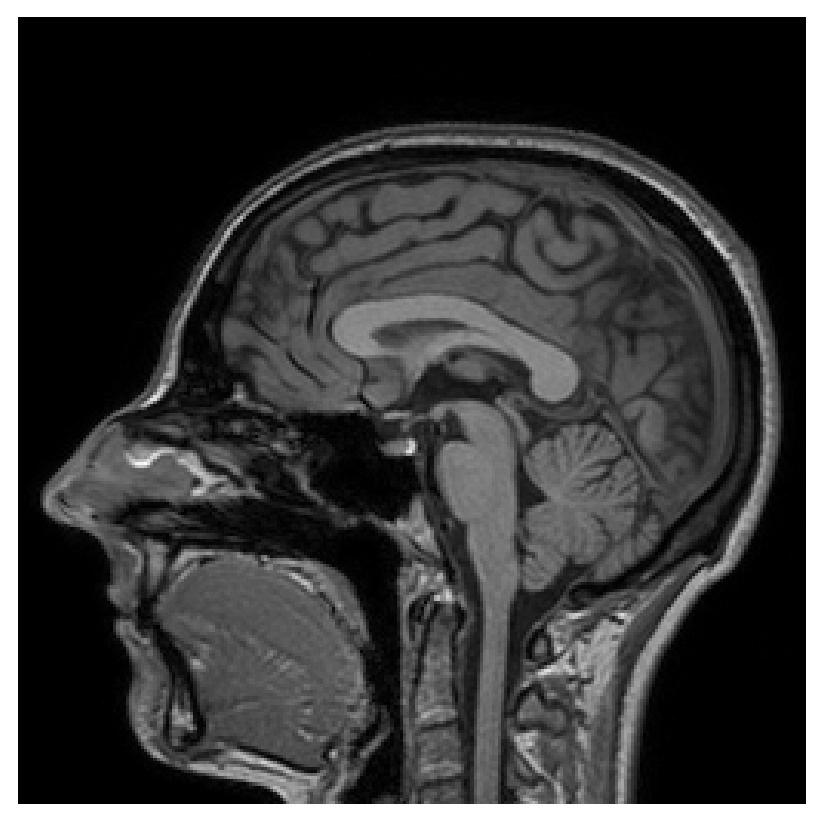
\includegraphics[width=\textwidth]{smoothing2D_decimationFactor51_orig}
     \caption{$\fat{T}$}
  \end{subfigure}
  \hfill
  \begin{subfigure}{0.45\textwidth}
     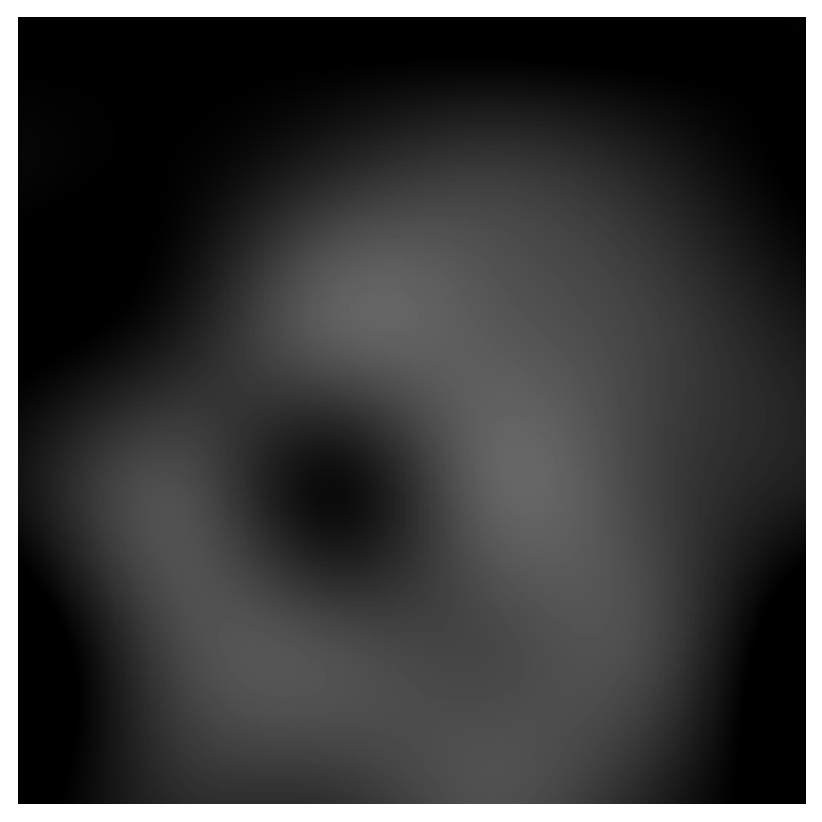
\includegraphics[width=\textwidth]{smoothing2D_decimationFactor51_smoothingNaive}
     \caption{
     %$\fat{\hat{T}} = \fat{S}_1 \fat{T} \fat{S}_2\transp$
     $\fat{\hat{T}}$
     }
  \end{subfigure}
  \begin{subfigure}{0.45\textwidth}
     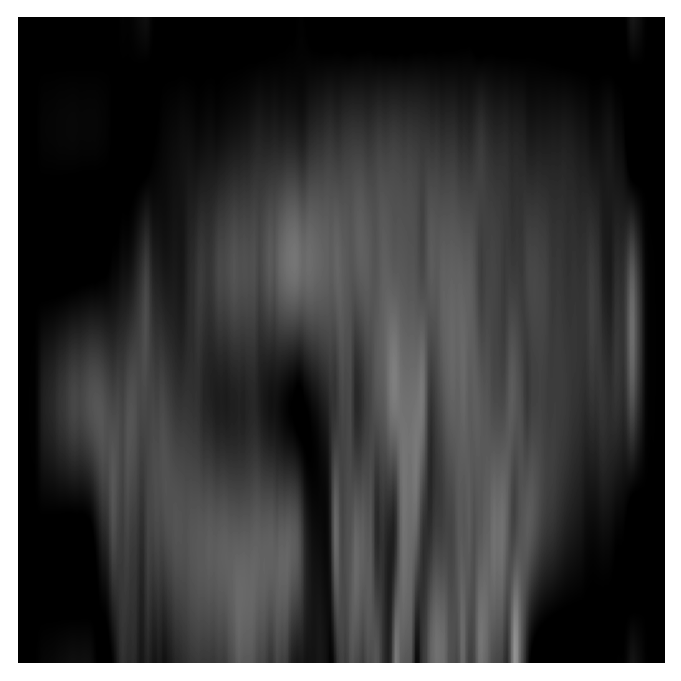
\includegraphics[width=\textwidth]{smoothing2D_decimationFactor51_smoothingRowWise}
     \caption{$\fat{S}_1 \fat{T}$}
  \end{subfigure}
  \hfill
  \begin{subfigure}{0.45\textwidth}
     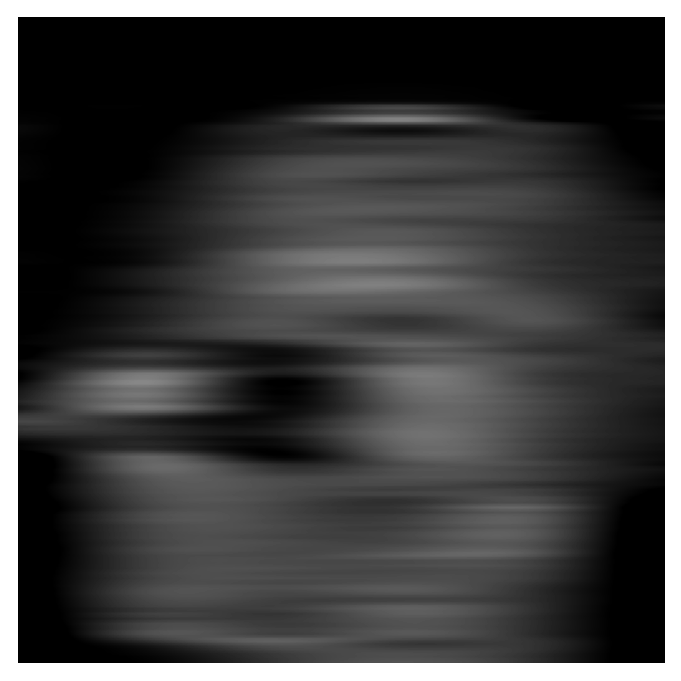
\includegraphics[width=\textwidth]{smoothing2D_decimationFactor51_smoothingColumnWise}
     \caption{$\fat{T} \fat{S}_2\transp$}
  \end{subfigure}
  \caption{%
  Smoothing of a 2D image $\fat{T}$ by fitting the 2D basis functions of Fig.~\ref{fig:basisFunctions2D_BSpline} to it. Computationally the smoothed result $\fat{\hat{T}}$ can be obtained by smoothing across the rows and then the columns (or vice versa), using the 1D basis functions shown in Fig.~\ref{fig:basisFunctions2D_BSpline}.
  }
  \label{fig:smoothing2D}
\end{figure}



\subsection{Interpolation in 2D}
\label{sec:interpolationIn2D}

For interpolation, the parameters are simply obtained as 
$$
\fat{W} = \bldgr{\Phi}_1^{-1} \fat{T} \left(\bldgr{\Phi}_2^{-1}\right)\transp 
.
$$
Interpolated values at new locations $\fat{x}$ are then computed using~\eqref{eq:prediction}, exploiting the separability of the basis functions~\eqref{eq:basisFunction2D}. 
Nearest-neighbor, linear and cubic interpolation in 2D are illustrated in Fig.~\ref{fig:interpolation2D}.

\begin{figure}
  \centering
  \begin{subfigure}[b]{0.48\textwidth}
     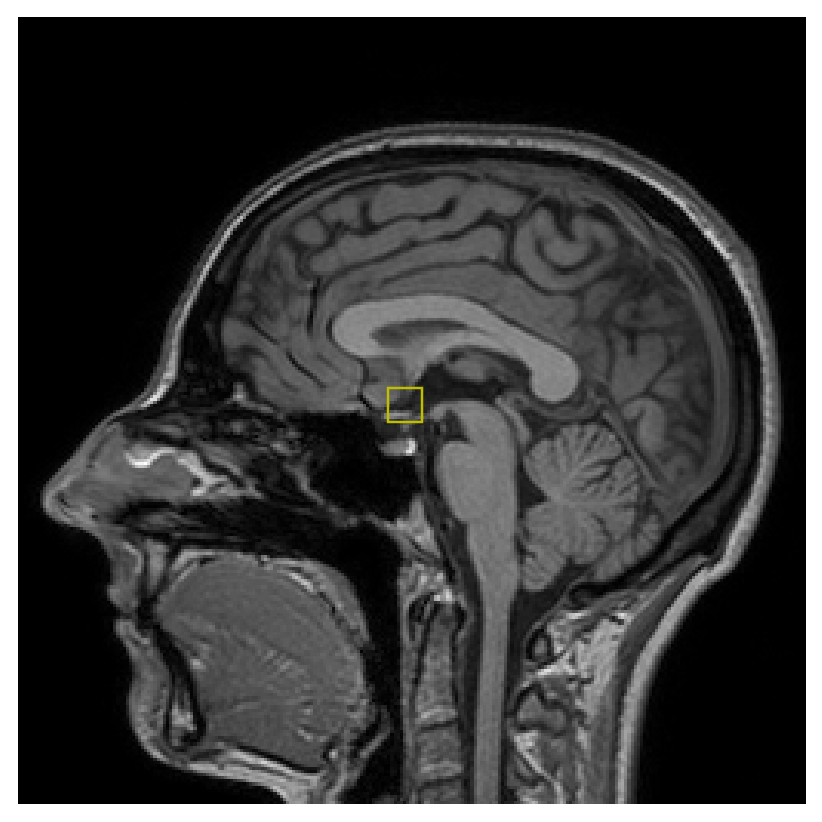
\includegraphics[width=\textwidth]{interpolation2D_areaIndication}
     \caption{}
     \label{fig:interpolation2D_areaIndication}
  \end{subfigure}
  \hfill
  \begin{subfigure}[b]{0.48\textwidth}
     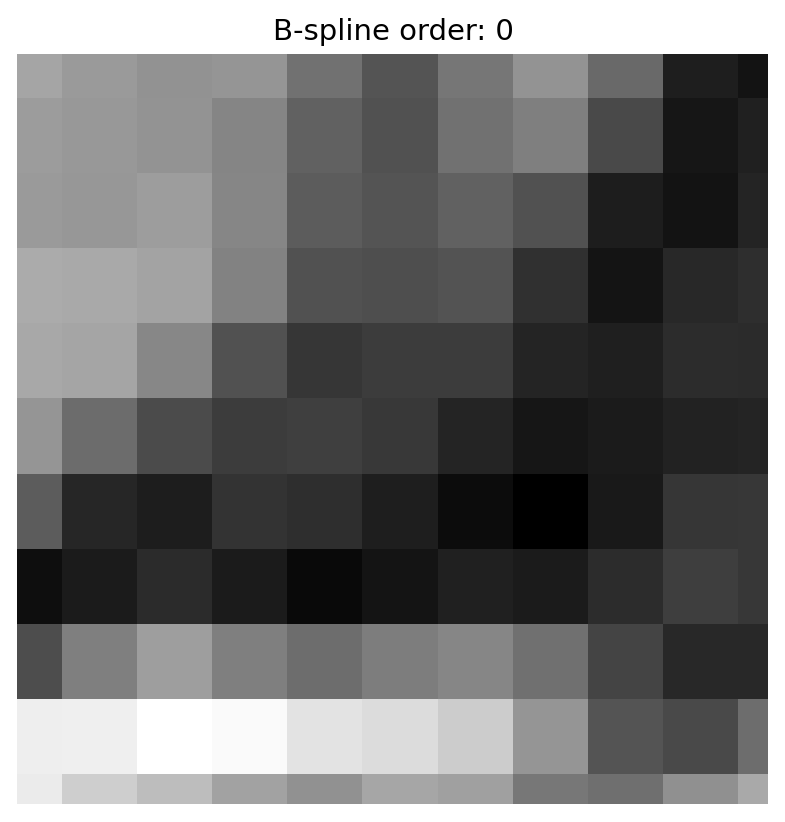
\includegraphics[width=\textwidth]{interpolation2D_BSplineOrder0}
     \caption{}
     \label{fig:interpolation2D_BSplineOrder0}
  \end{subfigure}
  \begin{subfigure}[b]{0.48\textwidth}
     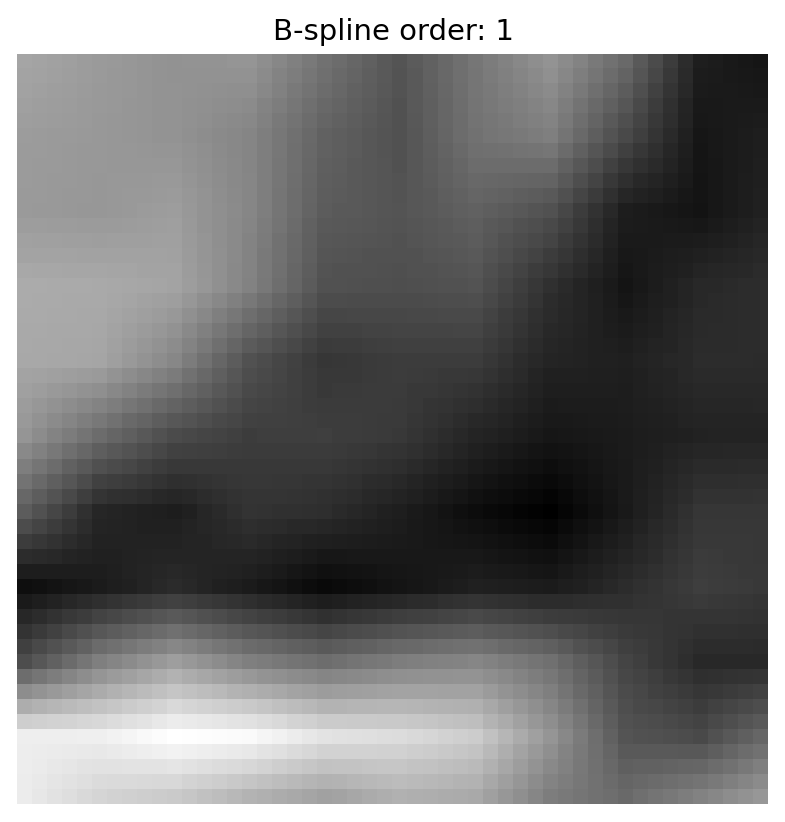
\includegraphics[width=\textwidth]{interpolation2D_BSplineOrder1}
     \caption{}
     \label{fig:interpolation2D_BSplineOrder1}
  \end{subfigure}
  \hfill
  \begin{subfigure}[b]{0.48\textwidth}
     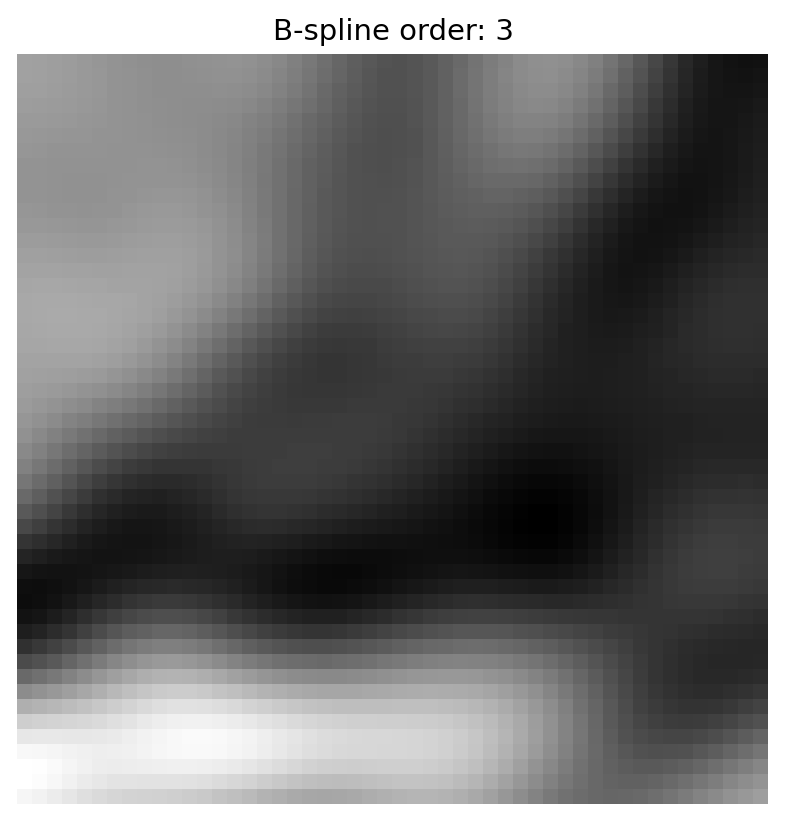
\includegraphics[width=\textwidth]{interpolation2D_BSplineOrder3}
     \caption{}
     \label{fig:interpolation2D_BSplineOrder3}
  \end{subfigure}
  \caption{2D nearest-neighbor~(\subref{fig:interpolation2D_BSplineOrder0}), linear~(\subref{fig:interpolation2D_BSplineOrder1}) and cubic~(\subref{fig:interpolation2D_BSplineOrder3}) interpolation within the small image area indicated in~(\subref{fig:interpolation2D_areaIndication}).}
  \label{fig:interpolation2D}
\end{figure}


\fi

\if\hideChapterRegistration0
\chapter{Image Registration}
\label{chap:registration}


\noindent
% In image registration, corresponding locations two or more images 
In many situations, the information contained in two or more images needs to be combined. Examples of such situations include interpreting images of the same patient acquired at different time points, or with different imaging modalities, as well as comparing the anatomy or function between various subject groups (e.g., to study how patients differ from controls in a clinical research study).
%
In order for images to be used this way, they need to be \emph{spatially aligned} so that corresponding structures appear in corresponding locations. The process of aligning images is called \emph{image registration}. This chapter introduces some of its basic concepts in a medical imaging context.


\section{Coordinate systems}

% 
% https://nipy.org/nibabel/coordinate_systems.html
% 
%  - "voxel coordinates"
%  - "The voxel coordinate tells us almost nothing about where the data came from 
%     in terms of position in the scanner. [...] This is because the scanner allows
%     us to collect voxel data in almost any arbitrary position and orientation within
%     the magnet."
%  - "the voxel coordinates in the EPI image refer to different locations in the magnet 
%     to the voxel coordinates in the anatomical image."
%  - "voxel space"
%  - "scanner RAS+ coordinates to voxel coordinates"
%  - "There are conventions other than RAS+ for the reference space. For example, DICOM 
%     files map input voxel coordinates to coordinates in scanner LPS+ space."
%
% https://www.slicer.org/wiki/Coordinate_systems
%
%  - "Anatomical coordinate system": RAS vs. LPS
%  - "Image coordinate system": (i,j,k)
%  - This technique requires that the matrix A is augmented with an extra row of zeros at 
%    the bottom, an extra column-the translation vector-to the right, and a '1' in the lower
%    right corner. Additionally all vectors have to be written as homogeneous coordinates, 
%    which means that a '1' is augmented at the end." 
%
% https://se.mathworks.com/help/medical-imaging/ug/medical-image-coordinate-systems.html
%  - "the intrinsic coordinate system and the world, or patient, coordinate system."
%  - Medical image files store a transformation matrix to map intrinsic coordinates (i, j, k) 
%    to patient coordinates (x, y, z), and each file format has a different convention that 
%    defines the positive direction of each axis.
% 
% https://surfer.nmr.mgh.harvard.edu/fswiki/CoordinateSystems
%  
% https://imaging.mrc-cbu.cam.ac.uk/imaging/Transforming_SPM_world_coordinates_to_voxel_coordinates
%  - "Getting from SPM world coordinates (mm) to voxel coordinates"
%

So far we have taken a rather cavalier attitude regarding the spatial locations of voxels (pixels in 3D): for 3D images we have simply assumed that we can index individual voxels by their location $\fat{x} = (x_1, x_2, x_3)\transp$, where $x_1$, $x_2$ and $x_3$ are integers. In reality, however, scanners can generate images with almost any voxel size (spacing between the voxels in each of the three dimensions) and in any orientation. In magnetic resonance imaging (MRI), for instance, it is not uncommon to acquire multiple images when a patient is inside the scanner, each defined on its own image grid. An example is shown in Fig.~\ref{fig:voxelVsWorldCoordinates}.

\begin{figure}
  \centering
  \begin{subfigure}{\textwidth}
     \centering
     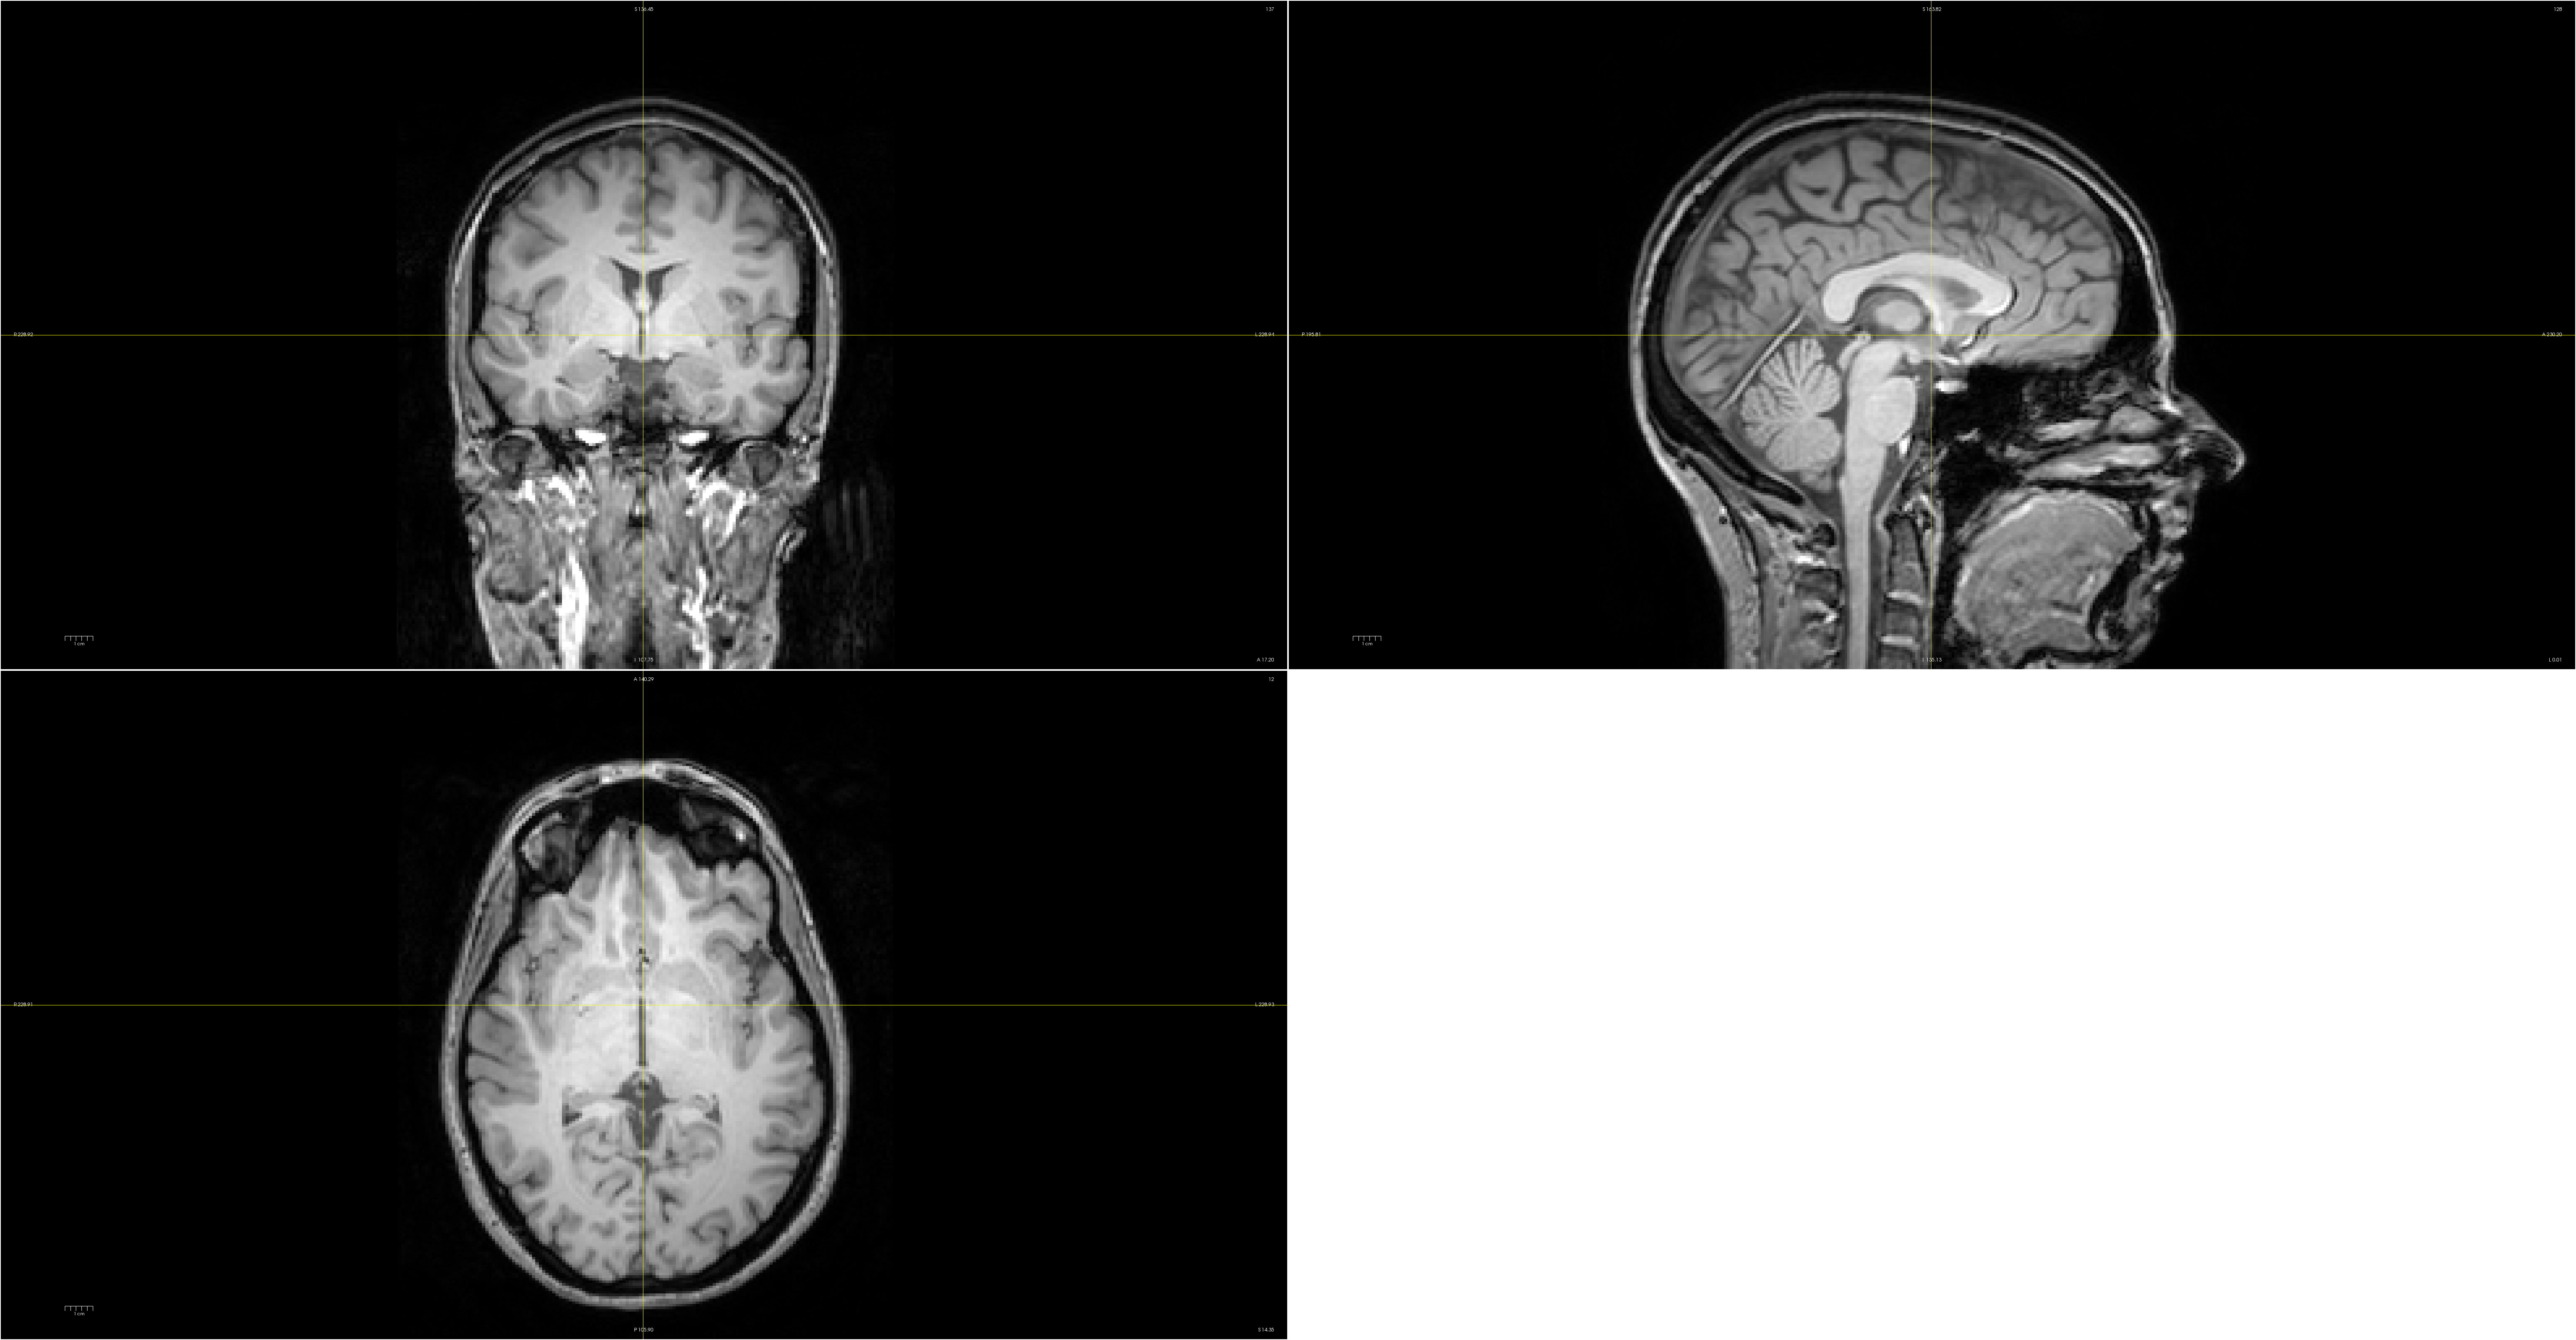
\includegraphics[width=0.49\textwidth]{T1_worldCoordinates}
     \hfill
     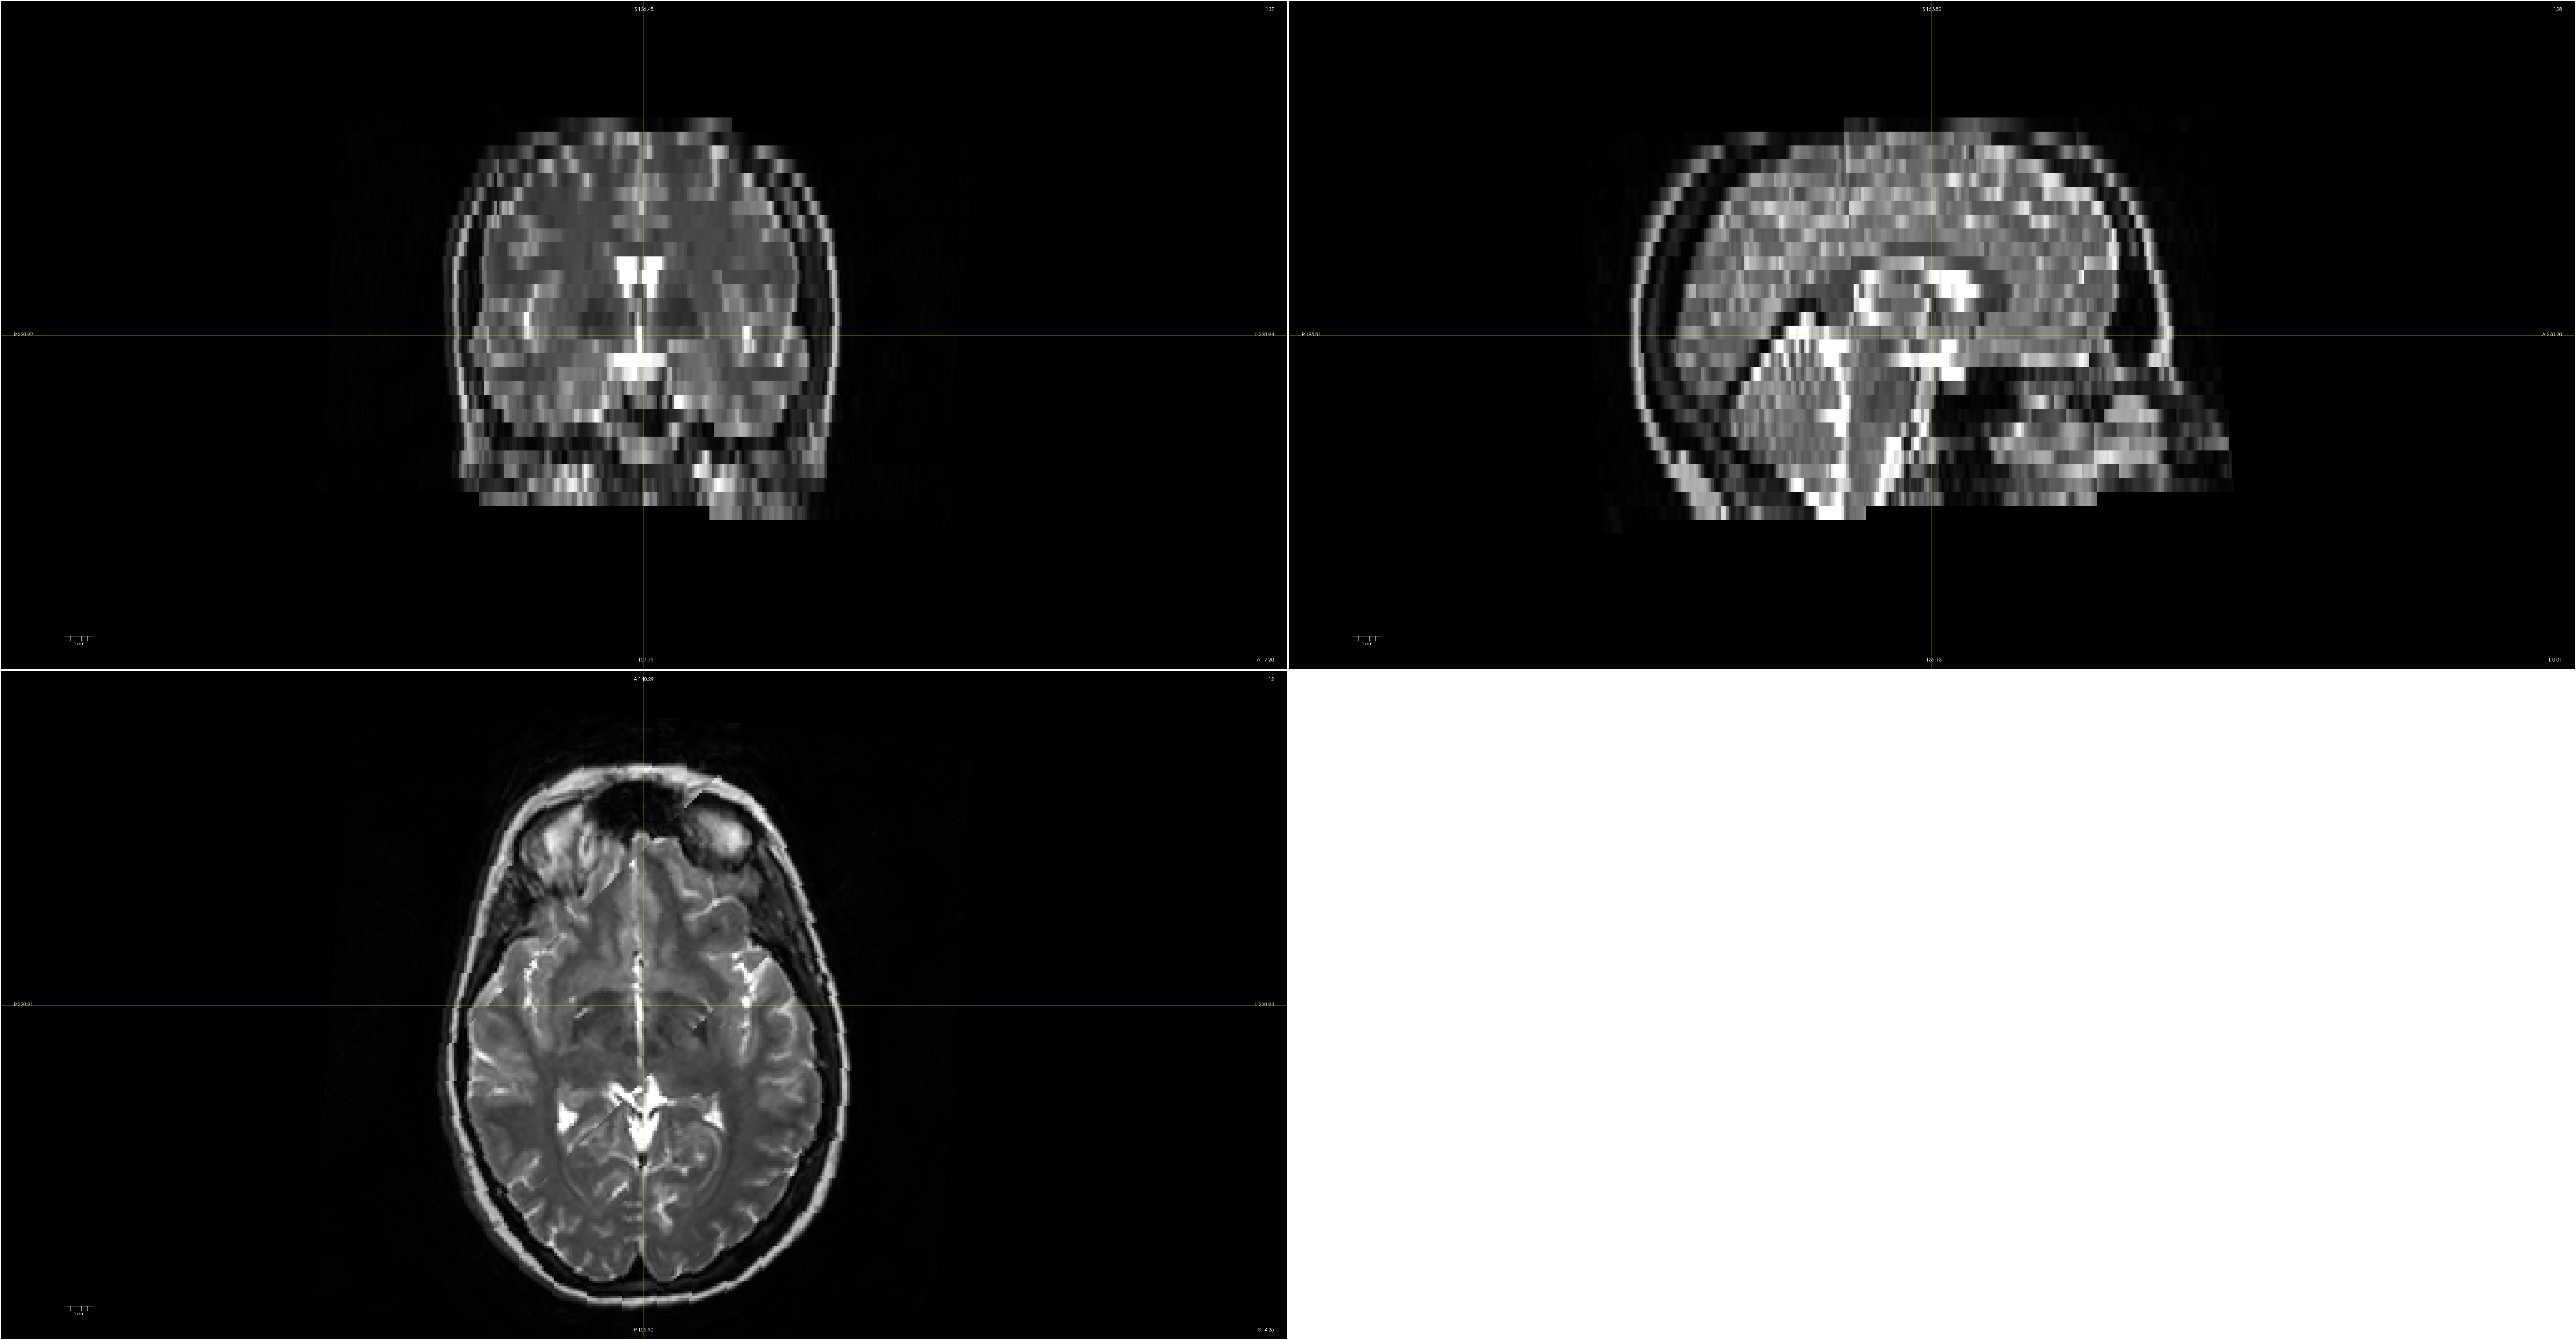
\includegraphics[width=0.49\textwidth]{T2_worldCoordinates}
     \caption{Displayed in world coordinates\\[5ex]}
     \label{fig:voxelVsWorldCoordinates_world}
  \end{subfigure}
  \begin{subfigure}{\textwidth}
     \centering
     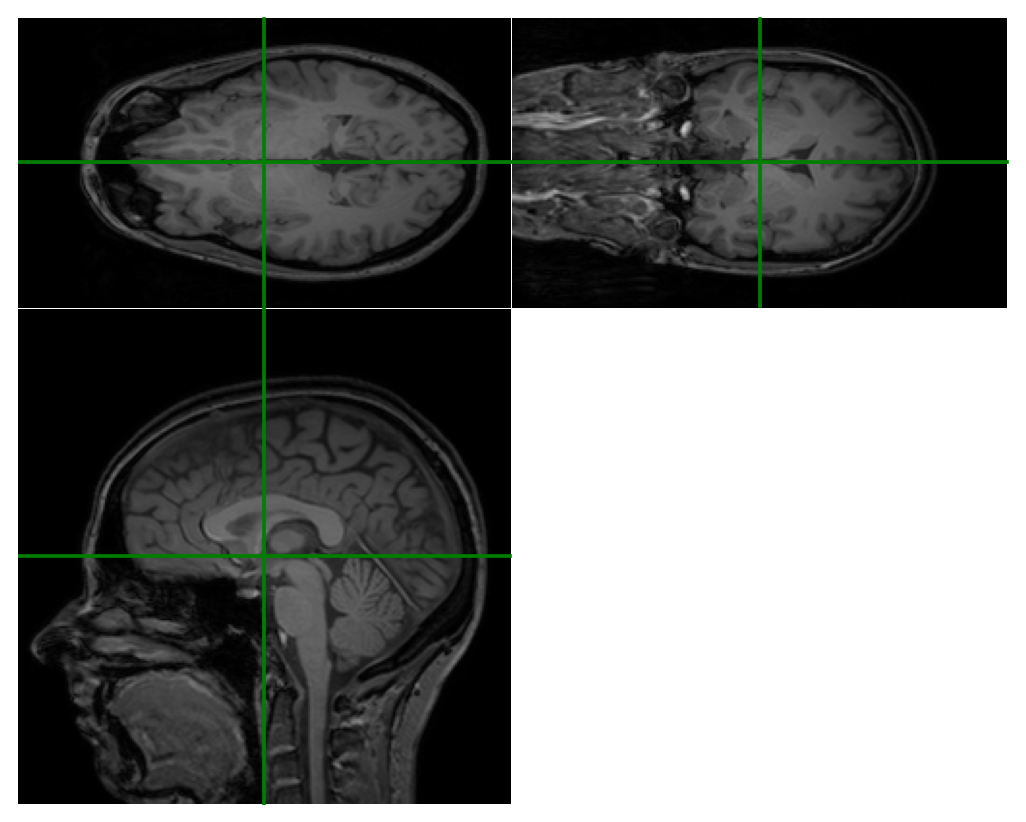
\includegraphics[width=0.48\textwidth]{T1_voxelCoordinates}
     \hfill
     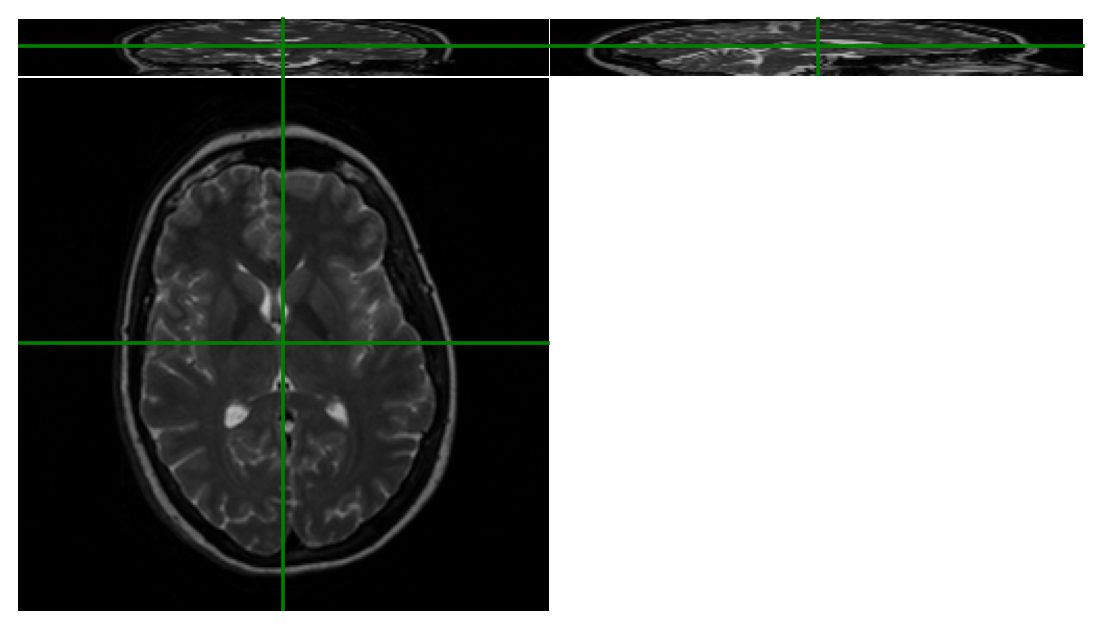
\includegraphics[width=0.48\textwidth]{T2_voxelCoordinates}
     \caption{Displayed in voxel coordinates}
     \label{fig:voxelVsWorldCoordinates_voxel}
  \end{subfigure}
  \caption{
  % T1: (256, 256, 150), 0.937500, 0.937500, 1.200000, sagittal.
  % T2: 256 x 256 x 28, 0.898438, 0.898438, 4.977778, axial
  Two MR images acquired within the same scan session: T1-weighted (left) and T2-weighted (right).
  Although the two images show corresponding structures in corresponding locations in \emph{world coordinates} (\subref{fig:voxelVsWorldCoordinates_world}), the 3D array of image intensities acquired by the scanner is actually very different between the two scans: The T1-weighted scan is a $256 \times 256 \times 150$ volume with voxel size $0.94 \times 0.94 \times 1.2\ mm^3$ acquired in the sagittal direction, whereas T2-weighted scan is a $256 \times 256 \times 28$ volume with voxel size $0.90 \times 0.90 \times 4.98\ mm^3$ acquired in the axial direction.
  This is clearly visible when displaying the two images in \emph{voxel coordinates} instead (\subref{fig:voxelVsWorldCoordinates_voxel}).
  }
  \label{fig:voxelVsWorldCoordinates}
\end{figure}

%
In order to 
relate 
multiple images 
% of the same anatomy 
to each other, we'll need to differentiate the concept of ``voxel coordinates'' (which are defined in integers units, and index individual voxels in a 3D image grid) from that of 
``world coordinates'' (indicating the spatial positions of voxels in the real world, and measured in mm).
%
Specifically, let $\fat{v} = (v_1, v_2, v_3)\transp$ denote the voxel coordinate of a voxel in an image of size $N_1 \times N_2 \times N_3$, where $v_d = 0, \ldots N_d-1$ for 
all dimensions 
$d=1, \ldots, 3$. 
%
In addition to a 
$N_1 \times N_2 \times N_3$ 
array of intensities,
the scanner will also encode a $3 \times 3$ matrix $\fat{A}$ and a $3 \times 1$ vector $\fat{t}$ to map voxel coordinates into world coordinates as follows:
\begin{equation}
\fat{x} = \fat{A} \fat{v} + \fat{t}
,
\label{eq:coordinateSystem}
\end{equation}
where
\begin{equation}
\fat{A} = 
\left(
\begin{array}{ccc}
a_{1,1} & a_{1,2} & a_{1,3} \\
a_{2,1} & a_{2,2} & a_{3,3} \\
a_{3,1} & a_{3,2} & a_{3,3}
\end{array}
\right)
\quad
\text{and}
\quad
\fat{t}
=
\left(
\begin{array}{c}
t_1 \\
t_2 \\
t_3
\end{array}
\right)
.
\label{eq:affineParameterization}
\end{equation}
For instance, the combination 
$$
\fat{A} = 
\left(
\begin{array}{ccc}
0.95 & 0    & 0 \\
0    & 0.95 & 0 \\
0    & 0    & 4.5
\end{array}
\right)
\quad
\text{and}
\quad
\fat{t}
=
\left(
\begin{array}{c}
-120.0 \\
-120.0 \\
-65.0 \\
\end{array}
\right)
$$
for an image of size $256 \times 256 \times 30$
would indicate that the size of a voxel is 0.95mm $\times$ 0.95mm $\times$ 4.5 mm, and that the origin of the world coordinate system (the location where $\fat{x} = \fat{0}$) 
% 0.95 * 127.5 = 121.125
% 4.5 * 14.5 = 65.25
lies somewhere in the middle of the image array. Very often, $\fat{A}$ will also include more general spatial transformations, such as 3D rotations or ``flipping'' of axes (negative voxel spacings, so that an increase in some voxel coordinate(s) will results in a \emph{decrease} in world coordinate(s)).

Who decides what directions $\fat{A}$ should encode, or where the origin of the world coordinate system should be located? This is a matter of convention, and several such conventions exist. The origin is often considered to be approximately at the center of the anatomical structure being scanned; a well-known world coordinate system is the RAS convention, where $x_1$ increases towards the \textbf{\underline{R}}ight of the patient, $x_2$ towards the \textbf{\underline{A}}nterior (front), and $x_3$ towards the \textbf{\underline{S}}uperior (top) of the patient. Another often-used convention is LPS (\textbf{\underline{L}}eft, \textbf{\underline{P}}osterior, \textbf{\underline{S}}uperior), which is similar to the RAS system but with the direction of the first two axes swapped.
When working with medical images, it is critically important to know what convention is used for each image, lest a patient be operated on the wrong side of their body!


%
Consider again the situation in Fig.~\ref{fig:voxelVsWorldCoordinates}, where two different images of the same patient 
% (each with its own system $\{\fat{A},\fat{t}\}$) 
were acquired within the same scanning session: one T1-weighted scan 
with voxel-to-world mapping 
$\{\fat{A}_{T1},\fat{t}_{T1}\}$,
and one T2-weighted scan 
with 
$\{\fat{A}_{T2},\fat{t}_{T2}\}$.
In order to compute the voxel coordinate $\fat{v}_{T2}$ in the T2-weighted scan corresponding to a 
%specific anatomical location with 
voxel coordinate $\fat{v}_{T1}$ in the T1-weighed one, it is often convenient to re-write~\eqref{eq:coordinateSystem} as follows:
\begin{equation}
\left(
\begin{array}{c}
x_1 \\
x_2 \\
x_3 \\
1
\end{array}
\right)
= 
\underbrace{
\left(
\begin{array}{cccc}
a_{1,1} & a_{1,2} & a_{1,3} & t_1 \\
a_{2,1} & a_{2,2} & a_{2,3} & t_2 \\
a_{3,1} & a_{3,2} & a_{3,3} & t_3 \\
0 & 0 & 0 & 1
\end{array}
\right)
}_{\fat{M}}
\left(
\begin{array}{c}
v_1 \\
v_2 \\
v_3 \\
1
\end{array}
\right)
,
\label{eq:affineMatrix}
\end{equation}
where the $4 \times 4$ matrix $\fat{M}$ is called an \emph{affine} matrix.
This technique, which uses so-called homogeneous coordinates (vectors are augmented with a $1$ at the end), absorbs the addition of the vector $\fat{t}$ into a single matrix multiplication, which makes concatenating several affine matrices very easy:  
the mapping of $\fat{v}_{T1}$ to $\fat{v}_{T2}$ is given by:
$$
\left(
\begin{array}{c}
\fat{v}_{T2} \\
1 
\end{array}
\right)
=
\fat{M}_{T2}^{-1}
\cdot
\fat{M}_{T1}
\cdot
\left(
\begin{array}{c}
\fat{v}_{T1} \\
1 
\end{array}
\right)
.
$$
%
We will soon see examples where more than two affine matrices are combined this way.

\section{Transformation models}

% 
% Maes talks about floating and reference image (= the one being interpolated)
% 
% Wells talks about reference volume and test volume [ so ``reference'' is opposite of Maes!]
% 
% Klein (Elastix) uses fixed and moving image 
% 

In many situations, images will not be perfectly aligned as in Fig.~\ref{fig:voxelVsWorldCoordinates}. This could be because the patient has moved between the two acquisitions, for instance because the scanning was performed on a different day or on a different scanner (e.g., MRI vs. CT scan). It could also be because of organ deformation, caused by breathing in a dynamic MRI, for instance, or because of tumor shrinkage or patient weight loss during the course of a radiation therapy treatment. In such situations, an additional geometrical transformation exists that a registration method should try to recover so that the images can still be compared to each other.

Let $\fat{x}=(x_1, \ldots, x_D)\transp$ denote a spatial location (in world coordinates) in an image that we will call the \emph{fixed} image in the remainder,
where $D=2$ in 2D and $D=3$ in 3D images.
Similarly, we will use $\fat{y}=(y_1, \ldots, y_D)\transp$ to denote 
% the corresponding 
spatial locations (again in world coordinates) in another image, which we will refer to as the \emph{moving} image. Our task is to find a transformation model
\begin{equation}
\fat{y}( \fat{x}, \fat{w} ) 
=
\left(
\begin{array}{c}
y_1( \fat{x}, \fat{w} ) \\
\vdots \\
y_D( \fat{x}, \fat{w} ) \\
\end{array}
\right)
\label{eq:mapping}
\end{equation}
so that points 
% at $\fat{x}$ 
in the fixed image are mapped to the corresponding anatomical locations 
% $\fat{y}$ 
in the moving image.
% 
Here $y_d( \fat{x}, \fat{w})$ is a function that governs how points 
in the fixed image
move along the $d$-th direction
in the moving image as the 
% this function is controlled by a 
parameter vector $\fat{w}$
is varied.
% for each dimension;  
% The vector $\fat{w} = (\fat{w}_1\transp, \ldots, \fat{w}_D\transp)\transp$ collects all the transformation parameters of the entire $D$-dimensional model.








\subsection{Linear transformations}

% 
% Affine with concatenation; Rigid with possible decomposiion
% 

\paragraph{Affine transformation:}
In the most general form of linear transformations, lines that are straight in the fixed image will still be straight when mapped into the moving image, but angles and areas/volumes are typically not preserved. 
An illustration is provided in Fig.~\ref{fig:affine}.
Such transformations are useful to roughly align images of different individuals or time points (for instance as a first step in a subsequent nonlinear registration algorithm), so that the major differences in size and orientation are removed. The transformation model is governed by:
$$
\fat{y}( \fat{x}, \fat{w} ) = \fat{A} \fat{x} + \fat{t}
,
$$
where $\fat{A}$ and $\fat{t}$ are given by
$$
\fat{A} = 
\left(
\begin{array}{cc}
a_{1,1} & a_{1,2} \\
a_{2,1} & a_{2,2} 
\end{array}
\right)
\quad
\text{and}
\quad
\fat{t}
=
\left(
\begin{array}{c}
t_1 \\
t_2
\end{array}
\right)
$$
in 2D,
and by~\eqref{eq:affineParameterization} in 3D.
Here $\fat{t}$ implements a translation, whereas rotation, scaling and skewing are 
% obtained through 
encoded in
$\fat{A}$.
%
This transformation model is called the \emph{affine} transformation model.
%
Referring to~\eqref{eq:mapping},
the $d$-th coordinate of points mapped into the moving image is therefore given by the linear function
\begin{equation}
y_d( \fat{x}, \fat{w}_d ) = t_d + a_{d,1} x_1 + \ldots + a_{d,D} x_D 
,
\label{eq:affineOneDirection}
\end{equation}
with parameters $\fat{w}_d = (t_d, a_{d,1}, \ldots, a_{d,D})\transp$.
Note that these parameters only contain elements of the $d$-th row of $\fat{A}$ and $\fat{t}$;
the vector $\fat{w} = (\fat{w}_1\transp, \ldots, \fat{w}_D\transp)\transp$ collects all the transformation parameters of the entire $D$-dimensional model.


In 3D, the affine matrix notation of~\eqref{eq:affineMatrix} can be used to compute the mapping of a voxel coordinate $\fat{v}_F$ in the fixed image into the corresponding voxel coordinate 
$\fat{v}_M$ in the moving image as follows:
\begin{equation}
\fat{v}_M
=
\fat{M}_M^{-1}
\cdot
\fat{M}
\cdot
\fat{M}_F
\cdot
\fat{v}_F
,
\label{eq:affineVoxelToVoxel}
\end{equation}
where $\fat{M}_F$ and $\fat{M}_M$ denote the voxel-to-world affine matrix of the fixed and the moving image, respectively.

\begin{figure}
  \centering
  \begin{subfigure}{\textwidth}
     \centering
     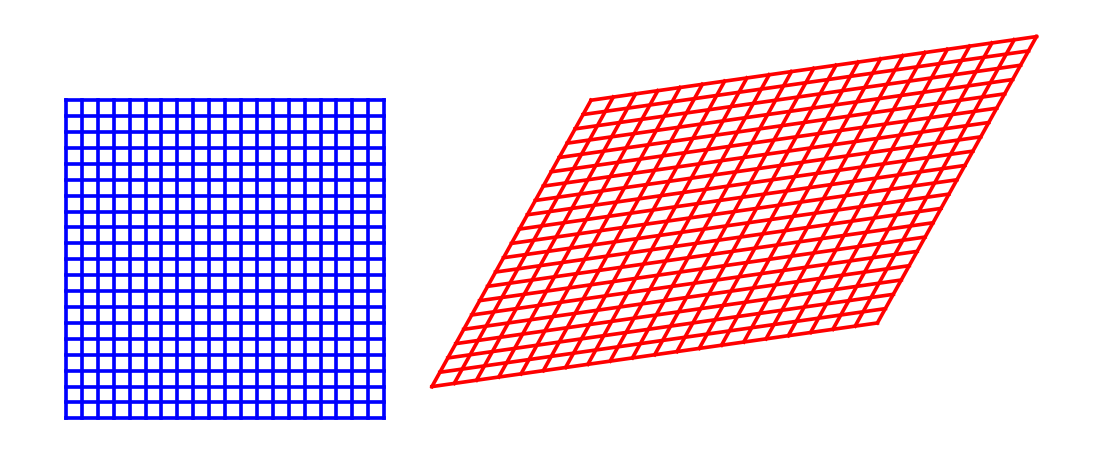
\includegraphics[width=0.8\textwidth]{affine}
     \caption{Affine transformation}
     \label{fig:affine}
  \end{subfigure}
  \begin{subfigure}{\textwidth}
     \centering
     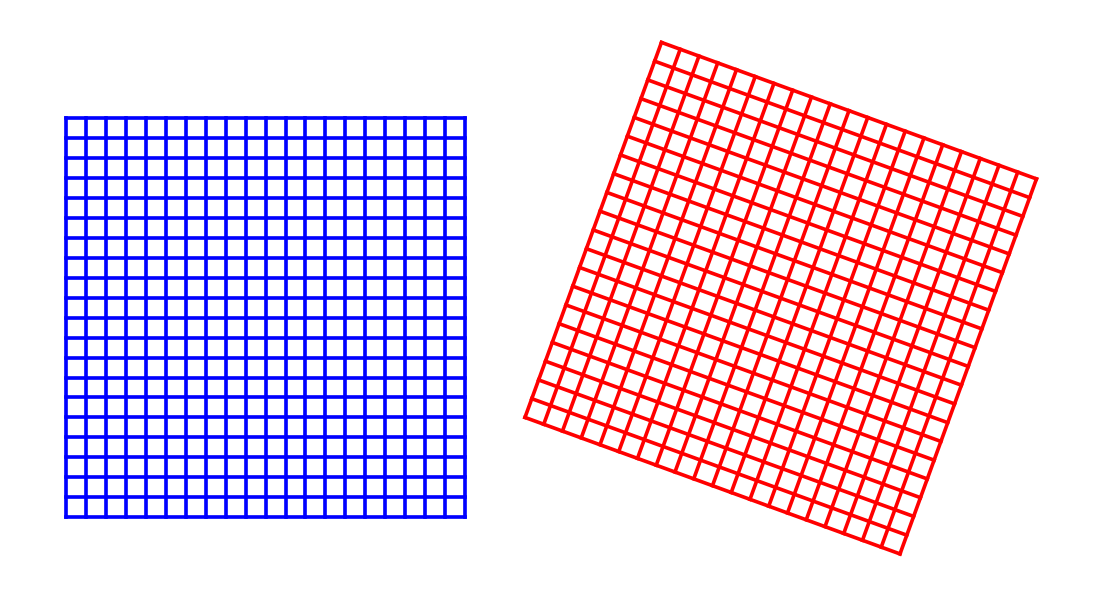
\includegraphics[width=0.8\textwidth]{rigid}
     \caption{Rigid transformation}
     \label{fig:rigid}
  \end{subfigure}
  \begin{subfigure}{\textwidth}
     \centering
     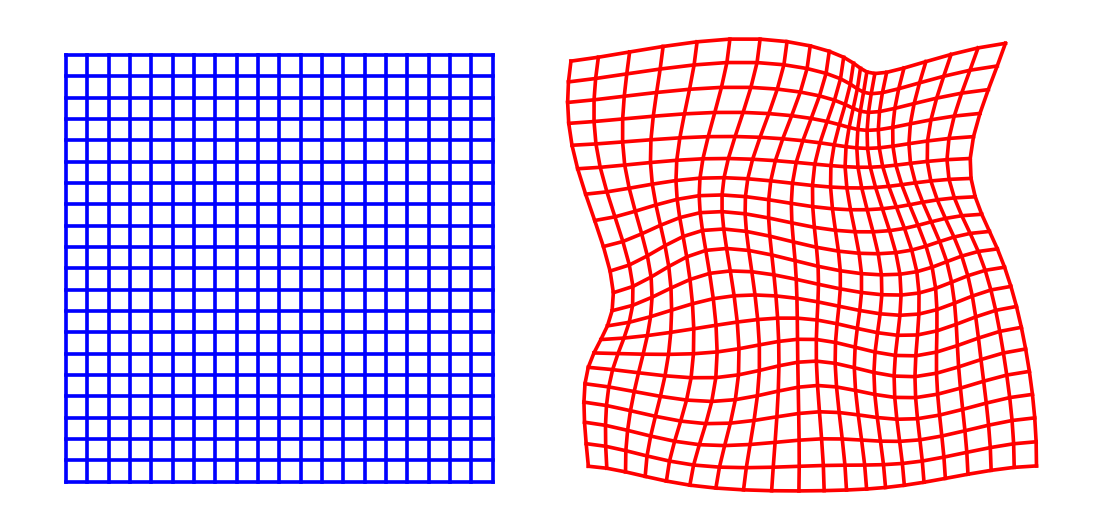
\includegraphics[width=0.8\textwidth]{nonlinear}
     \caption{Nonlinear transformation}
     \label{fig:nonlinear}
  \end{subfigure}
  \caption{Illustration of affine, rigid and nonlinear transformation models. The red grid shows how the regular grid shown in blue is characteristically mapped under each transformation model.}
  \label{fig:transformationModels}
\end{figure}  



\paragraph{Rigid transformation:}

In situations where the moving and the fixed image were both taken from the same rigid structure (e.g, the head) in the same subject, the ability of the affine transformation model to arbitrarily scale and skew images becomes a liability. In those cases, a model that can only account for a translation and a rotation is more appropriate:
$$
\fat{y}( \fat{x}, \fat{w} ) = \fat{R} \fat{x} + \fat{t},
$$
where $\fat{R}\transp \fat{R} = \fat{I}$ and $\det(\fat{R}) = 1$.
%
This transformation model is called the \emph{rigid} transformation model, and is illustrated in Fig.~\ref{fig:rigid}.
%
In 2D, rotations can be enforced by parameterizing the rotation matrix $\fat{R}$ as follows:
$$
\fat{R} 
=
\left(
\begin{array}{rr}
\cos(\alpha) & -\sin( \alpha ) \\
\sin( \alpha ) & \cos( \alpha )
\end{array}
\right)
,
$$
where $\alpha$ is a rotation angle.
The parameters of this model are therefore $\fat{w} = (\alpha, t_1, t_2)\transp$. 
In 3D there are many possible parametrizations of the rotation matrix, but one possibility is as follows:
{%
\footnotesize%
$$
%\footnotesize
\fat{R}
=
\left(
\begin{array}{rrr}
1 & 0 & 0 \\
0 & \cos( \gamma ) & -\sin( \gamma ) \\
0 & \sin( \gamma ) &  \cos( \gamma )
\end{array}
\right)
\cdot
\left(
\begin{array}{rrr}
\cos( \beta ) & 0 & -\sin( \beta ) \\
0 & 1 & 0 \\
\sin( \beta ) &  0 & \cos( \beta ) \\
\end{array}
\right)
\cdot
\left(
\begin{array}{rrr}
\cos( \alpha ) & -\sin( \alpha ) & 0 \\
\sin( \alpha ) &  \cos( \alpha ) & 0 \\
0 & 0 & 1
\end{array}
\right)
,
$$}%
where $\alpha$, $\beta$ and $\gamma$ are three rotation angles;
the parameters of the model are then given by $\fat{w} = ( \alpha, \beta, \gamma, t_1, t_2, t_3 )\transp$.

Provided 
% the elements of $\fat{R}$ are 
% % used to construct 
% filled into
% the affine matrix $\fat{M}$, 
the affine matrix $\fat{M}$
is constructed by using $\fat{A} = \fat{R}$,
\eqref{eq:affineVoxelToVoxel} remains valid to 
% compute voxel coordinates in the moving image from voxel coordinates in the fixed image.
map voxel coordinates in the fixed image into voxel coordinates in the moving image.



\subsection{Nonlinear transformations}

In situations where tissue deformation needs to be modeled, the linear function~\eqref{eq:affineOneDirection} (one for each dimension $d$)
in affine registration
is generalized 
% by using nonlinear basis functions 
to a nonlinear one.
% instead.
%
%Furthermore,
Since global differences in overall size and orientation have typically already been removed using a preceding affine registration\footnote{For instance by replacing the affine voxel-to-world mapping of the fixed image $\fat{M}_F$ by $\fat{M} \cdot \fat{M}_F$}, only the \emph{residual deformation} 
% $\delta_d(\fat{x}, \fat{w}_d)$
$\delta_d$
is modeled:
\begin{equation}
y_d( \fat{x}, \fat{w}_d ) = x_d + \delta_d(\fat{x}, \fat{w}_d),
\quad
\text{where}
\quad
\delta_d(\fat{x}, \fat{w}_d) =
\sum_{m=0}^{M-1} w_{d,m} \phi_m( \fat{x} )
.
\label{eq:deformableOneDirection}
\end{equation}
Here $\phi_m(\fat{x})$ are $M$ basis functions, which are typically taken to be \emph{separable} (cf.~\eqref{eq:basisFunction2D} and Fig.~\ref{fig:basisFunctions2D_BSpline}),
with weights $\fat{w}_d = (w_{d,0}, \ldots w_{d,M-1})\transp$.
%
The interpretation of these weights is that, when they are all set to zero (i.e., when $\fat{w}_d = \fat{0}$), the deformation $\delta_d$ is also zero and no deformation is applied.
An illustration of a nonlinear transformation encoded this way is provided in Fig.~\ref{fig:nonlinear}.

%
It is worth reiterating that the motion of points along each individual dimension $d$ in the moving image is governed by its own set of parameters $\fat{w}_d$.
%
In 2D, there will therefore by two sets of parameters: $\fat{w} = (\fat{w}_1, \fat{w}_2)\transp$,
whereas in 3D there will be three: $\fat{w} = (\fat{w}_1, \fat{w}_2, \fat{w}_3 )\transp$.




\section{Landmark-based registration}

One way to register two images is by manually annotating corresponding points in both images, and then finding a spatial transformation that brings matching point pairs close to each other. Letting $\{\fat{x}_n\}_{n=1}^N$ denote a set of $N$ point locations annotated in the fixed image, and $\{\fat{y}_n\}_{n=1}^N$ the corresponding locations in the moving image, 
registration can be obtained by minimizing
the energy
$$
E(\fat{w}) 
=
\sum_{n=1}^N \| \fat{y}_n - \fat{y}( \fat{x}_n, \fat{w} ) \|^2
$$
with respect to the transformation parameters $\fat{w}$. 
Here $\| \fat{a} - \fat{b}\|^2 = \sum_{d=1}^D (a_d-b_d)^ 2$ measures the squared Euclidean distance between two points $\fat{a}$ and $\fat{b}$.

\paragraph{Affine transformation:}
%
Optimizing $E(\fat{w})$ with respect to $\fat{w}$ will be particularly straightforward when the mapping in each dimension $d$ is governed by its own set of parameters $\fat{w}_d$,
% in a linear fashion,
as is the case in both the affine and nonlinear formulation of~\eqref{eq:affineOneDirection} and~\eqref{eq:deformableOneDirection}.
This is because the energy can then be split into a sum of $D$ independent energies, one for each dimension: 
\begin{eqnarray*}
E( \fat{w} ) 
& = & 
\sum_{n=1}^N 
\sum_{d=1}^D
\left[ y_{n,d} - y_d( \fat{x}_n, \fat{w}_d ) \right]^2 
\\
& = & 
\sum_{d=1}^D E_d( \fat{w}_d )
\quad
\text{with}
\quad
E_d( \fat{w}_d )
=
\sum_{n=1}^N 
\left[ y_{n,d} - y_d( \fat{x}_n, \fat{w}_d ) \right]^2
,
\end{eqnarray*}
where $y_{n,d}$ denotes the $d$-th element of $\fat{y}_n$.
%
Optimizing each $E_d(\fat{w}_d)$ with respect to $\fat{w}_d$ is easy: 
in both the affine and the nonlinear case, 
$\fat{y}_d( \fat{x}_n, \fat{w}_d )$ is only \emph{linearly} dependent on $\fat{w}_d$,
reducing the problem to the form of linear regression analyzed in Sec.~\ref{sec:linearRegression}.
%
Taking affine registration as an example, the energy for the $d$-th dimension is given by (cf.~\eqref{eq:affineOneDirection}) 
$$
E_d(\fat{w}_d) = 
\sum_{n=1}^N 
\left[ y_{n,d} - t_d - a_{d,1} x_{n,1} - \ldots - a_{d,D} x_{n,D} \right]^2
,
$$
which is minimized at solution
\begin{equation}
\left( 
\begin{array}{c}
t_d \\
a_{d,1} \\
\vdots \\
a_{d,D}
\end{array}
\right)
=
\left( \fat{X}\transp \fat{X} \right)^{-1} \fat{X}\transp 
\left(
\begin{array}{c}
y_{1,d} \\
\vdots \\
y_{N,d}
\end{array}
\right)
,
\label{eq:pointBasedAffineSolution}
\end{equation}
where
$$
\fat{X} =
\left(
\begin{array}{cccc}
1      & x_{1,1} & \cdots & x_{1,D} \\ 
1      & x_{2,1} & \cdots & x_{2,D} \\ 
\vdots & \vdots  & \ddots & \vdots  \\
1      & x_{N,1} & \cdots & x_{N,D}
\end{array}
\right)
.
$$
%
The $d$-th row of the affine transformation parameters $\fat{A}$ and $\fat{t}$ is therefore given by~\eqref{eq:pointBasedAffineSolution}. 
Doing this for all $D$ dimensions yields all the required parameter values.


\paragraph{Rigid transformation:}
%
Optimizing $E(\fat{w})$ with respect to $\fat{w}$ is more involved when a rigid transformation model is used, since the constraints 
% on the rotation matrix 
that $\fat{R}\transp\fat{R} = \fat{I}$ and 
$\det(\fat{R})=1$ prevent us from decoupling the problem across dimensions.
For the translation vector $\fat{t}$ this is not yet an issue, and 
we can therefore use the same approach as before to deduce that, for a given rotation $\fat{R}$, the energy
\begin{equation}
E(\fat{w}) = \sum_{n=1}^N \| \fat{y}_n - \fat{R} \fat{x}_n - \fat{t} \|^2
\label{eq:energyRigid}
\end{equation}
is minimized when 
% $$
% \fat{t} = \fat{\bar{y}} - \fat{R} \fat{\bar{x}},
% \quad
% \text{with}
% \quad
% \fat{\bar{y}} = \frac{1}{N} \sum_{n=1}^N \fat{y}_n
% \quad
% \text{and}
% \quad
% \fat{\bar{x}} = \frac{1}{N} \sum_{n=1}^N \fat{x}_n
% .
% $$
\begin{equation}
\fat{t} = \fat{\bar{y}} - \fat{R} \fat{\bar{x}},
\label{eq:solutionForTranslationInRigid}
\end{equation}
where
$
\fat{\bar{y}} = \frac{1}{N} \sum_{n=1}^N \fat{y}_n
$
and
$
\fat{\bar{x}} = \frac{1}{N} \sum_{n=1}^N \fat{x}_n
$.
% 
Plugging this result into~\eqref{eq:energyRigid}, we can reformulate the energy as
$$
E(\fat{w}) = \sum_{n=1}^N \| \fat{\tilde{y}}_n - \fat{R} \fat{\tilde{x}}_n \|^2
\quad 
\text{where}
\quad
\fat{\tilde{y}}_n = \fat{y}_n \! - \! \fat{\bar{y}}
\quad 
\text{and}
\quad
\fat{\tilde{x}}_n = \fat{x}_n \! - \! \fat{\bar{x}}
.
$$
Under the constraint $\fat{R}\transp\fat{R} = \fat{I}$, this is minimized when~\cite{schonemann1966generalized}
$$
\fat{R} = \fat{V} \fat{U}\transp, 
$$
where $\fat{U}$ and $\fat{V}$ are $D \times D$ matrices such that
$$
\fat{U}\transp \fat{U} = \fat{I},
\quad
\fat{V}\transp \fat{V} = \fat{I}
\quad
\text{and}
\quad
\sum_{n=1}^N \fat{\tilde{x}}_n \fat{\tilde{y}}_n\transp 
=
\fat{U}
\bldgr{\Sigma}
\fat{V}\transp
,
$$
where $\bldgr{\Sigma}$ is diagonal.
%
One such a solution is obtained by computing the singular value decomposition (SVD) of the matrix 
$\sum_{n=1}^N \fat{\tilde{x}}_n \fat{\tilde{y}}_n\transp$.
% which yields a $\bldgr{\Sigma}$ with non-negative values on the diagonal. 
However, this solution does not necessarily satisfy the second constraint of rotational matrices that 
$\det( \fat{R} ) = 1$. It is also possible\footnote{%
Since $\det(\fat{A} \fat{B}) = \det(\fat{A}) \det(\fat{B})$,
we have that $\det(R) = \det(U) \det(V)$.
Furthermore,
$\det(\fat{U}) \pm 1$ and $\det(\fat{V}) \pm 1$ since $\fat{U}\transp \fat{U} = \fat{I}$ and $\fat{V}\transp \fat{V} = \fat{I}$.
}
that $\det( \fat{R} ) = -1$, in which case a valid rotation can be obtained by ``flipping'' one of the columns of $\fat{R}$ by reversing the sign of all the elements in it.

Once $\fat{R}$ has been found, \eqref{eq:solutionForTranslationInRigid} can be used to find the remaining parameters $\fat{t}$.



\section{Intensity-based registration}

% 
% SSD, MI. Say something about optimization
% 

Landmark-based registration suffers from a number of shortcomings, including the need for manually annotating images and the fact that registrations are computed from only a handful of points. This limits both the efficiency and the accuracy with which images can be aligned.

Another class of algorithms can perform registrations fully automatically, by minimizing energies that are computed directly from raw image intensities. Below we review two well-known methods in this family.

\subsection{Sum of squared differences}
\label{sec:ssd}


When the fixed and the moving image both depict the same anatomical structures with the same (or very similar) intensity characteristics, a successful registration will be characterized by small differences in absolute intensity values at corresponding locations. Scenarios where this idea can be used include co-registering two CT scans, where intensity values have a direct physical interpretation, or two MR images acquired with similar pulse sequences on similar hardware (e.g., T1-weighted images acquired at different time points or from different subjects on the same scanner).
In the latter case, 
images will often still need to be pre-processed to make their intensities comparable (for instance by intensity rescaling), since MR scanners do not typically provide measurements in quantitative physical units.

%
On a technical level,
registration can be obtained by minimizing the sum of squared differences in intensities at corresponding locations:
\begin{equation}
E(\fat{w}) 
=
\sum_{n=1}^N 
\left[ 
% \mathcal{M}( \fat{y}( \fat{x}_n, \fat{w} ) ) - \mathcal{F}( \fat{x}_n )
\mathcal{F}( \fat{x}_n ) - \mathcal{M}( \fat{y}( \fat{x}_n, \fat{w} ) )
\right]^2
.
\label{eq:SSD}
\end{equation}
Here, $\fat{x}_n$ are the world coordinates of the voxels in the \emph{fixed} image, and $\mathcal{F}(\fat{x}_n)$ denotes the image intensity of those voxels.
Similarly, $\mathcal{M}( \fat{y}( \fat{x}_n, \fat{w} ) )$ denotes the image intensities in the \emph{moving} image, evaluated at the mapped locations $\fat{y}( \fat{x}_n, \fat{w} )$. Since these will generally fall in between original voxel locations in the moving image, image interpolation will be required (cf.~Sec.~\ref{sec:interpolationIn2D}). When the mapped location falls \emph{outside} of the image area of the moving image, a constant intensity will typically be assigned (for instance zero).

\subsubsection{Gauss-Newton optimization}
%
Unlike in landmark-based registration, finding parameter values $\fat{w}$ that
minimize the energy~\eqref{eq:SSD} is no longer given by closed-form solutions, and numerical optimization methods need to be used. 
% 
When the number of parameters of the transformation model is low, for instance in rigid or affine registration, generic optimization algorithms that only evaluate $E(\fat{w})$ (and perhaps its gradient $\nabla E(\fat{w})$) will work quite well.
%
For cases with many degrees of freedom, such as flexible nonlinear deformations, a dedicated optimization ``trick'' can be used that exploits the specific structure of the energy~\eqref{eq:SSD}
to obtain faster solutions.

%
The method is known as \emph{Gauss-Newton}, and involves linearizing $\mathcal{M}( \fat{y}( \fat{x}_n, \fat{w} ) )$ with respect to $\fat{w}$ around the current parameter values.
%
Specifically, for the nonlinear transformation model of~\eqref{eq:deformableOneDirection}, where deformations are encoded in each dimension $d$ separately, the partial derivative of $\mathcal{M}( \fat{y}( \fat{x}_n, \fat{w} ) )$ with respect to $w_{d,m}$ is given by (chain rule):
\begin{equation}
\frac{\partial \mathcal{M}( \fat{y}( \fat{x}_n, \fat{w} ) )}{\partial w_{d,m}}
=
%\underbrace{
\frac{\partial \mathcal{M}( \fat{y}( \fat{x}_n, \fat{w} ) )}{\partial y_d}
%}_{g_{d,n}}
%\cdot
\,\,
\frac{\partial y_d( \fat{x}_n, \fat{w}_d )}{\partial w_{d,m}}
=
g_{d,n} 
% \cdot 
\,\,
\phi_m( \fat{x}_n )
.
\label{eq:partialDerivative}
\end{equation}
Here the fact that $\frac{\partial y_d( \fat{x}_n, \fat{w}_d )}{\partial w_{d,m}} = \phi_m( \fat{x}_n )$ was used, and the notation
$g_{d,n} = \frac{\partial \mathcal{M}( \fat{y}( \fat{x}_n, \fat{w} ) )}{\partial y_d}$ 
was introduced as shorthand for the partial spatial derivative of the moving image 
in the $d$-th dimension,
% (in world coordinates), 
% with respect to the $d$-th component of the world coordinate
evaluated at 
% point $\fat{y} = \fat{y}( \fat{x}_n, \fat{w} )$.
position $\fat{y}( \fat{x}_n, \fat{w} )$.
%
By using a cubic B-spline interpolation model, such spatial derivatives can be conveniently computed everywhere~\cite{thevenaz2000interpolation}. 
%


\iffalse
$$
\frac{\partial \mathcal{M}( \fat{y}( \fat{x}_n, \fat{w} ) )}{\partial w_{d,m}}
=
\underbrace{\frac{\partial \mathcal{M}( \fat{y}( \fat{x}_n, \fat{w} ) )}{\partial y_d}}_{\nabla_{n,d}}
% \cdot
\underbrace{\frac{\partial y_d( \fat{x}_n, \fat{w}_d )}{\partial w_{d,m}}}_{\phi_m( \fat{x}_n )}
,
$$

$$
\frac{\partial \mathcal{M}( \fat{y}( \fat{x}_n, \fat{w} ) )}{\partial w_{d,m}}
=
\frac{\partial \mathcal{M}( \fat{y}( \fat{x}_n, \fat{w} ) )}{\partial y_d}
% \cdot
\frac{\partial y_d( \fat{x}_n, \fat{w}_d )}{\partial w_{d,m}}
.
$$

the fact that $\frac{\partial y_d( \fat{x}_n, \fat{w}_d )}{\partial w_{d,m}} = \phi_m( \fat{x}_n )$
\fi

For a small deviation $\bldgr{\epsilon}$ from some parameter values $\fat{w}$, 
\eqref{eq:partialDerivative} can now be used in a first-order Taylor expansion to obtain the approximation
\begin{equation}
\mathcal{M}( \fat{y}( \fat{x}_n, \fat{w}+\bldgr{\epsilon} ) ) 
\simeq
\mathcal{M}( \fat{y}( \fat{x}_n, \fat{w} ) ) 
+ 
\sum_{d=1}^D \sum_{m=0}^M \big( g_{d,n} \phi_m( \fat{x}_n ) \big) \epsilon_{d,m}
.
\label{eq:taylor}
\end{equation}
Plugging this into the energy~\eqref{eq:SSD},
and defining 
$$
\tau_n = \mathcal{F}( \fat{x}_n ) - \mathcal{M}( \fat{y}( \fat{x}_n, \fat{w} ) )
$$
we obtain
$$
E( \fat{w} + \bldgr{\epsilon} )
\simeq
\sum_{n=1}^N
\left[
\tau_n - \sum_{d=1}^D \sum_{m=0}^M \big( g_{d,n} \phi_m( \fat{x}_n ) \big) \epsilon_{d,m}
\right]^2
,
$$
which can be recognized has having the form of a linear regression problem with parameters 
$\bldgr{\epsilon}$.
The value of $\bldgr{\epsilon}$ minimizing $E(\fat{w} + \bldgr{\epsilon})$
is therefore given by (cf.~Sec.~\ref{sec:linearRegression})
\begin{equation}
\bldgr{\epsilon}
=
\left( 
\bldgr{\Psi}\transp \bldgr{\Psi}
\right)^{-1}
\bldgr{\Psi}\transp
\bldgr{\tau}
\label{eq:GaussNewton}
\end{equation}
where 
$
\bldgr{\tau} = (\tau_1, \ldots, \tau_N)\transp
$
and 
$$
\bldgr{\Psi} =
\left(
\begin{array}{c|c|c}
\fat{G}_1 \bldgr{\Phi}
&
\cdots 
&
\fat{G}_D \bldgr{\Phi}
\end{array}
\right)
,
$$
where 
$\fat{G}_d = \mathrm{diag}( g_{d,n}, \ldots, g_{d,N} )$
and 
$\bldgr{\Phi}$ is given by~\eqref{eq:Phi}.

%
This result suggests the following simple iterative algorithm for optimizing $E(\fat{w})$:
\begin{enumerate}
 \item Select a starting value for the transformation parameters, e.g., $\fat{w}=\fat{0}$ (no deformation);
 \item Use~\eqref{eq:GaussNewton} to compute a small update $\bldgr{\epsilon}$ to the current parameters $\fat{w}$;
 \item Update the parameters: $\fat{w} \gets \fat{w} + \bldgr{\epsilon}$;
 \item Repeat steps 2. and 3. until convergence is detected.
\end{enumerate}
There is one catch, though:
In the derivation above, we have assumed that $\bldgr{\epsilon}$ is ``small''. What happens if we compute $\bldgr{\epsilon}$ and one or more of its components are actually quite large? Then our approximation~\eqref{eq:taylor} will have been a poor one, and we might find that the energy $E(\fat{w})$ \emph{increases} (instead of \emph{decreasing}) after we use $\bldgr{\epsilon}$ to update $\fat{w}$. To avoid such situations, several methods to modify $\bldgr{\epsilon}$ exist.
% to alter $\bldgr{\epsilon}$
One such a modification is the \emph{Levenberg-Marquardt} algorithm, which replaces~\eqref{eq:GaussNewton} by
\begin{equation}
\bldgr{\epsilon}
=
\left( 
\bldgr{\Psi}\transp \bldgr{\Psi}
+ \lambda \fat{I}
\right)^{-1}
\bldgr{\Psi}\transp
\bldgr{\tau}
\label{eq:Levenberg-Marquardt}
,
\end{equation}
where $\lambda \geq 0$ is a tunable parameter that is typically updated after each iteration. 
If the parameter update $\bldgr{\epsilon}$ does not decrease $E(\fat{w})$, the update is rejected and $\lambda$ is increased until a decrease in $E(\fat{w})$ is obtained; this will happen eventually because for very large $\lambda$ the algorithm devolves into a gradient-descent algorithm with a small step size.
Conversely, if $E(\fat{w})$ decreases a smaller $\lambda$ is used in the next iteration of the algorithm to improve efficiency.


\clearpage
\subsection{Mutual Information}

When two images need to be aligned that were acquired with two different imaging modalities (e.g., CT vs.~MR, or MR vs.~PET), the intensity characteristics of most anatomical structures will generally be quite different between the two images. This precludes the use of the sum-of-squared-differences energy as a registration criterion.

In such situations, fully automatic registrations can still be obtained by optimizing the \emph{Mutual Information} (MI) between the two images~\cite{wells1996multi,maes1997multimodality}. 
% 
For given transformation parameter values 
$\fat{w}$, the frequency with which specific \emph{discretized intensity pairs} $(f,m)$ occur 
% at corresponding locations 
is analyzed. 
%
Here, $f \in \{1, \ldots, B\}$ and $m \in \{1,\ldots,B\}$ denote intensities in the fixed and moving image, respectively, after both images have been preprocessed to only contain $B$ discrete intensity levels\footnote{Typically this is done by dividing the intensity range in each image into $B$ contiguous intervals, and recording the interval (``bin'') number of each voxel's intensity. Often-used values for $B$ are 32, 64 or 128.}.
%
More specifically, a \emph{joint histogram} 
$$
\fat{H}
=
\left(
\begin{array}{ccc}
h_{1,1} & \ldots & h_{1,B} \\ 
\vdots  & \ddots & \vdots \\
h_{B,1} & \ldots & h_{B,B}
\end{array}
\right)
$$
is computed,
where entry $h_{f,m}$ contains the number of times the intensity in the fixed image was $f$, while the corresponding intensity in the moving image was $m$. 
% This is done by
In practice, 
% $\fat{H}$ is computed by 
this is done by starting with an empty joint histogram 
% ($h_{f,m}\!=\!0, \,\, \forall f,m$), 
($\fat{H} = \fat{0}$), 
and filling it up by looping over all $N$ voxels in the fixed image. For each such voxel 
% $n=1,\ldots,N$, 
$n$,
its intensity $\mathcal{F}(\fat{x}_n)$ as well as the corresponding intensity in the moving image $\mathcal{M}(\fat{y}(\fat{x}_n, \fat{w}))$ is determined.  
%
The former will directly give us a value for $f$, but deciding on $m$ is more involved since $\fat{y}(\fat{x}_n, \fat{w})$ will typically fall somewhere between the voxels
in the moving image.
% a decision needs to be made  
An easy solution is to use nearest-neighbor interpolation, so that $m$ is simply the intensity of the voxel that is closest to $\fat{y}(\fat{x}_n, \fat{w})$; however in practice more involved schemes are typically used.
%
A related issue is what to do if $\fat{y}(\fat{x}_n, \fat{w})$ maps to a location outside of the image area of the moving image. In many implementations such voxels are simply skipped (i.e., they do not contribute to the joint histogram).
%
% In general, though, 
For most voxels, though,
a
valid intensity pair $(f,m)$ is obtained; 
% In any case, assuming a pair $(f,m)$ has been determined, the 
the corresponding joint histogram count $h_{f,m}$ is then increased by one, and the next voxel in the fixed image is visited.
An example of a joint histogram computed this way is shown in Fig.~\ref{fig:registration_joint}.

\begin{figure}
  \centering
  \begin{subfigure}{0.4\textwidth}
     \centering
     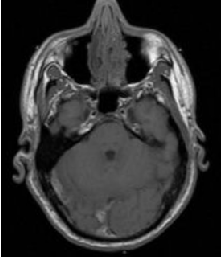
\includegraphics[width=\textwidth]{snapshot_plots__doInterModality_1__doMutualInformation_1__xOffset_0_MR}
     \caption{MR}
     \label{fig:registration_MR}
  \end{subfigure}
  \hfill
  \begin{subfigure}{0.4\textwidth}
     \centering
     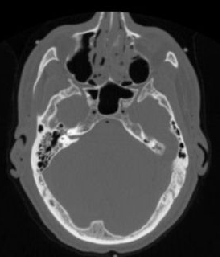
\includegraphics[width=\textwidth]{snapshot_plots__doInterModality_1__doMutualInformation_1__xOffset_0_CT}
     \caption{CT}
     \label{fig:registration_CT}
  \end{subfigure}
  \begin{subfigure}{0.4\textwidth}
     \centering
     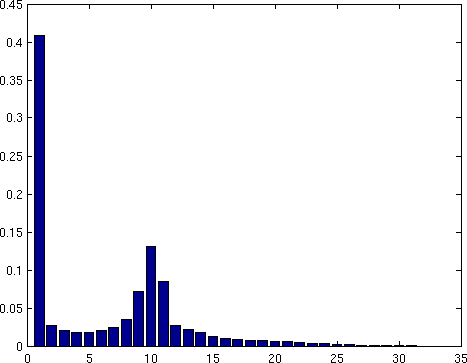
\includegraphics[width=\textwidth]{snapshot_plots__doInterModality_1__doMutualInformation_0__xOffset_0__marginal1}
     \caption{Marginal histogram (MR)}
     \label{fig:registration_MR_marginal}
  \end{subfigure}
  \hfill
  \begin{subfigure}{0.4\textwidth}
     \centering
     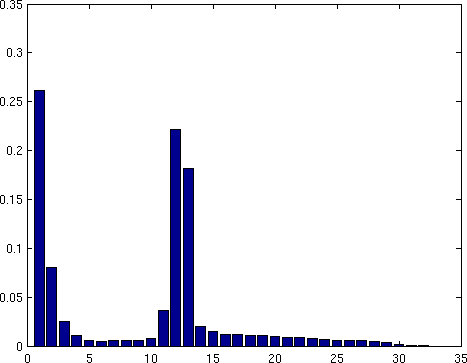
\includegraphics[width=\textwidth]{snapshot_plots__doInterModality_1__doMutualInformation_0__xOffset_0__marginal2}
     \caption{Marginal histogram (CT)}
     \label{fig:registration_CT_marginal}
  \end{subfigure}
  \begin{subfigure}{0.8\textwidth}
     \centering
     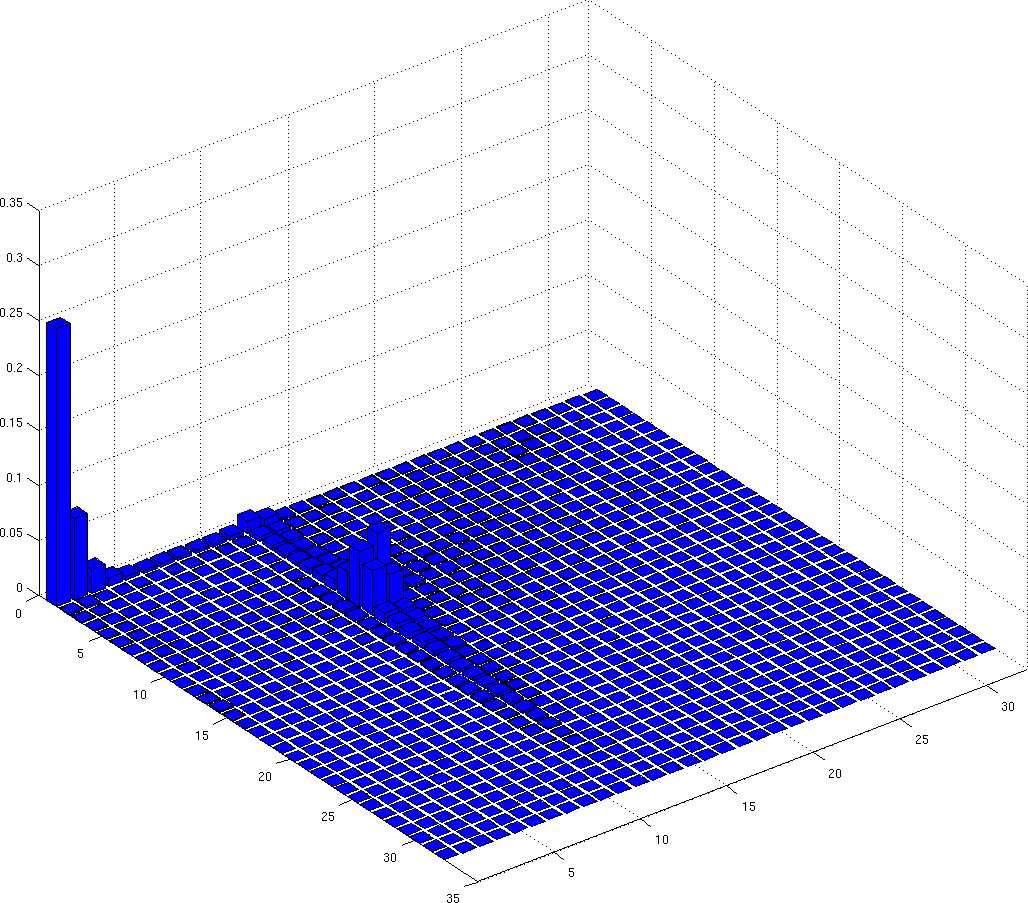
\includegraphics[width=\textwidth]{snapshot_plots__doInterModality_1__doMutualInformation_1__xOffset_0__pdf}
     \caption{Joint histogram}
     \label{fig:registration_joint}
  \end{subfigure}
  \caption{An MR and CT image in perfect alignment, along with their normalized (i.e., divided by $N$) joint and marginal histograms. The number of histogram bins was $B=32$.}
  \label{fig:registration_histograms}
\end{figure}





%
A key insight for registration purposes is that the joint histogram will typically have many entries with small counts when the two images are well aligned: most of the 
% $(f,m)$ 
encountered
intensity combinations $(f,m)$ will be concentrated in just a few histogram bins.
In contrast, when the images are moved out of alignment, intensity pairs will become more variable, ``smearing out'' the counts from high-count histogram entries into (what were previously) low-count bins. This process is illustrated in Fig.~\ref{fig:registration_histograms_blurring}.
%
This phenomenon can be exploited to define the 
% \emph{joint entropy} as a an energy to drive the registration process:
following registration energy:
$$
E(\fat{w}) 
= 
H_{F,M}%( \fat{w} ),
\quad
\text{with}
\quad
H_{F,M}%( \fat{w} ) 
= 
- 
\sum_{f=1}^B \sum_{m=1}^B
p_{f,m} 
\log( p_{f,m} ),
% \quad
% p_{f,m} = \frac{h_{f,m}}{N}
$$
where 
% $p_{f,m} = \frac{h_{f,m}}{N}$.
% $p_{f,m}$ are elements in the matrix $\fat{P} = \fat{H}/N$.
$p_{f,m} = h_{f,m} / N$ are normalized histogram counts.
%
These can be interpreted as \emph{probabilities} of seeing specific intensity combinations $(f,m)$
when the images are aligned with parameter value $\fat{w}$.
%
The quantity $H_{F,M}$ is known as the \emph{joint entropy} in information theory. It measures how predictable intensity combinations $(f,m)$ are, and is directly related to data compression: The more predictable the intensity combinations, the lower the joint entropy and the fewer bits will theoretically be needed to store or communicate the fixed-moving image pair.
%
Applied to our registration setting, the joint entropy will be higher when the joint histogram is ``smeared out'', which will happen when the images are not well aligned. This explains why $H_{F,M}$ can be used as an energy function to drive an automatic registration process.

\begin{figure}
  \centering
  \begin{subfigure}{0.8\textwidth}
     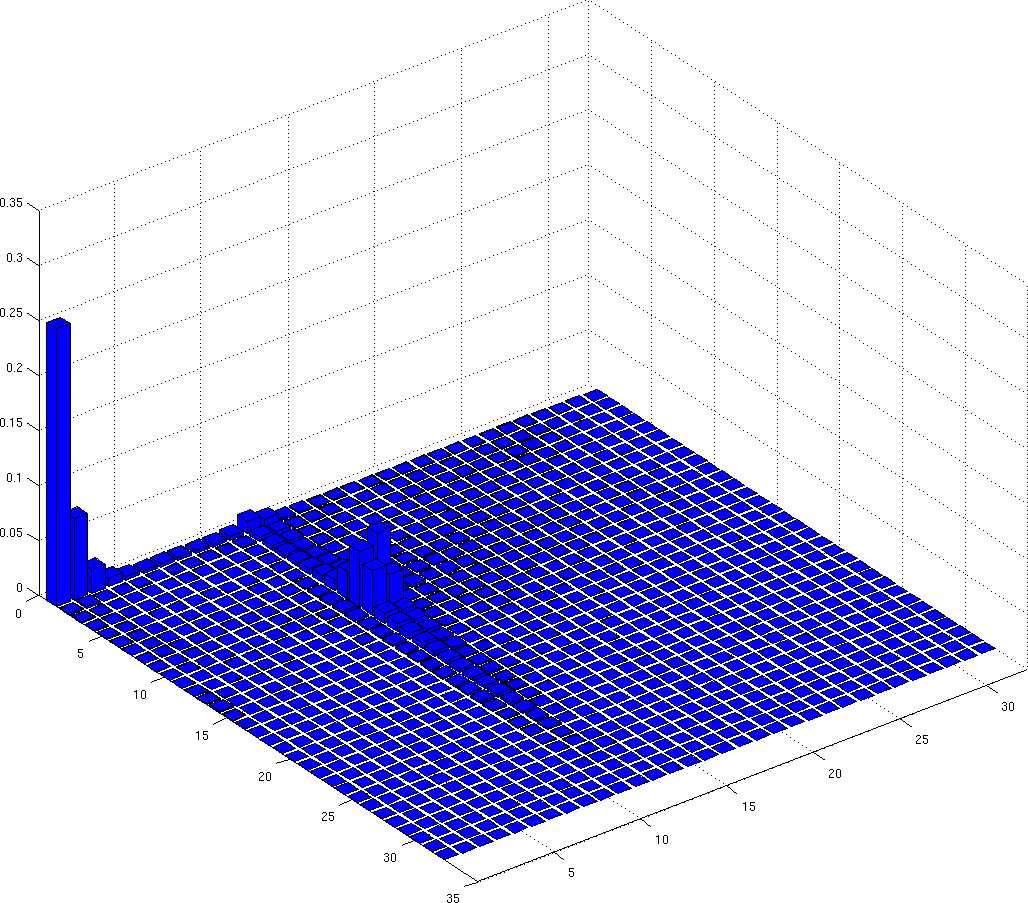
\includegraphics[width=\textwidth]{snapshot_plots__doInterModality_1__doMutualInformation_1__xOffset_0__pdf}
     \caption{}
     \label{fig:registration_histograms_blurring_perfect}
  \end{subfigure}
  \begin{subfigure}{0.8\textwidth}
     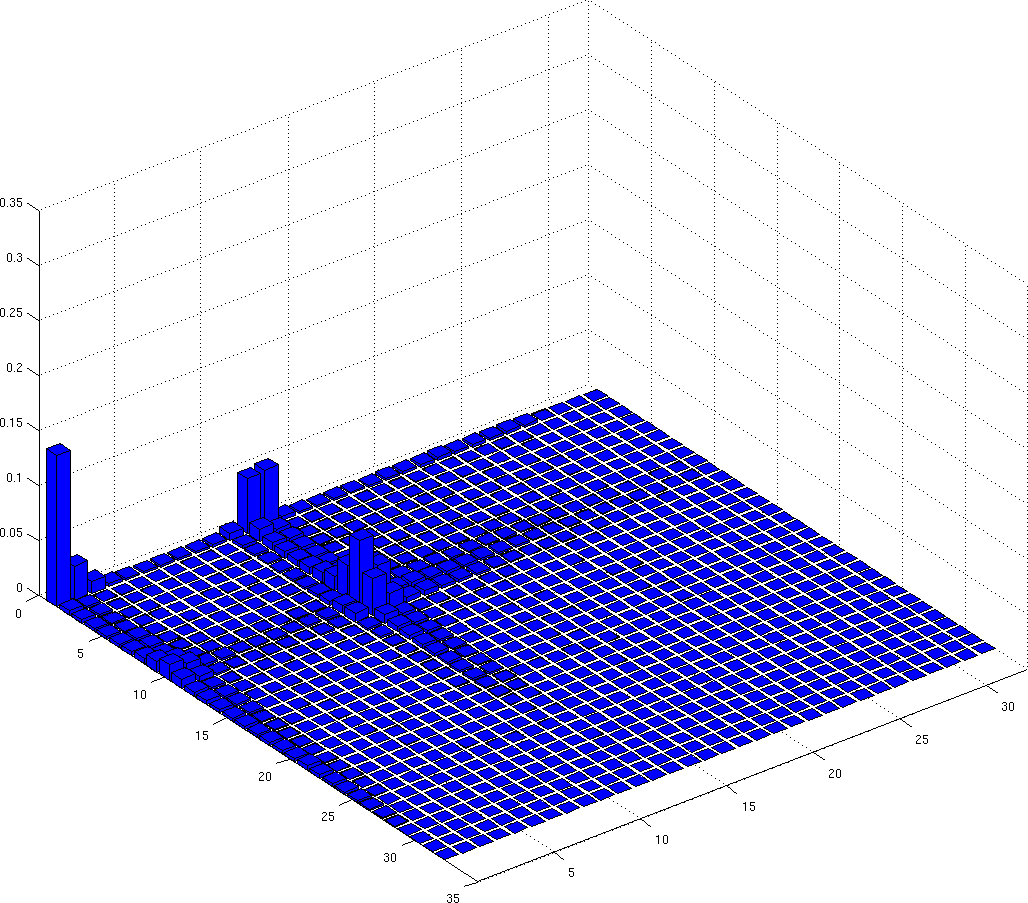
\includegraphics[width=\textwidth]{snapshot_plots__doInterModality_1__doMutualInformation_1__xOffset_-80__pdf}
     \caption{}
     \label{fig:registration_histograms_blurring_off}
  \end{subfigure}
  \caption{%
  Normalized joint histogram of the MR and CT scans shown in Fig.~\ref{fig:registration_histograms}, both when the images are in perfect alignment (\subref{fig:registration_histograms_blurring_perfect}) 
  and when the CT image is translated with respect to the MR image
  (\subref{fig:registration_histograms_blurring_off}).
  }
  \label{fig:registration_histograms_blurring}
\end{figure}



%
One problem with using the joint entropy is that it attains low values not just when registrations are good, but also when some non-desirable trivial solutions are found. As an example, consider the scenario where $\fat{w}$ is so that the fixed image and the moving image only overlap in a region in the background. In most implementations, the joint histogram is only computed from this overlapping region, as explained before, and therefore the only intensity pair with a non-zero count will be the one where both $f$ and $m$ are zero. The joint entropy for this solution will be zero, which is its lowest possible value.

In order to avoid such pathological solutions, it is customary to alter the energy as follows:
\begin{equation}
E(\fat{w}) = H_{F,M} - H_{F} - H_{M}
,
\label{eq:negativeMI}
\end{equation}
where $H_{F}$ and $H_{M}$ are the \emph{marginal entropies} of the fixed and moving image, respectively. 
They are defined as follows:
$$
H_{F} = -\sum_{f=1}^{B} p_f \log( p_f )
\quad
\text{and}
\quad
H_{M} = -\sum_{m=1}^{B} p_m \log( p_m ),
$$
where $p_f = \sum_{m=1}^B p_{f,m}$
%($p_m = \sum_{f=1}^B p_{f,m}$)
denotes the probability of encountering a voxel 
with intensity $f$
in the fixed image, 
%(moving image) 
%($m$).
and $p_m = \sum_{f=1}^B p_{f,m}$
the corresponding probability of encountering intensity $m$ in the moving image.
%
Adding these two terms to the energy function will steer the registration towards overlapping in areas that are ``interesting'' in both images, i.e., areas with actual content (with high marginal entropy).

Since the quantity
$
H_{F} + H_{M} - H_{F,M}  
$
is known in information theory as \emph{mutual information}, using its negative as energy function in~\eqref{eq:negativeMI} for registration purposes is known as \emph{mutual information-based registration}.
%
In a practical implementation, numerical optimization will need to be used to find values $\fat{w}$ with low energy. Currently these are mostly general-purpose optimizers that only need to be able to evaluate $E(\fat{w})$ and its gradient $\nabla E(\fat{w})$.































% \include{chapter1}
\newcounter{exerciseCounter}
\setcounter{exerciseCounter}{0}
% \include{chapter2}
% \include{chapter3}
% \include{chapter4}



\fi

\if\hideChapterModelBasedSegmentation0


\chapter{Model-based Segmentation}
\label{chap:modelBasedSegmentation}

The ability to efficiently delineate anatomical structures from medical images is important in many applications. Examples include measuring the number and volume of lesions and how they change over time, planning radiation therapy treatments or surgical interventions, and characterizing shape changes that occur in specific patient groups. The process of delineating structures is called \emph{image segmentation}, and automating it has traditionally been approached using model-based techniques. This chapter reviews some well-established techniques in this category.


\section{Generative models}

Image segmentation methods are often based on so-called \emph{generative} models, i.e., models that describe how images can be generated synthetically by random sampling from some probability distribution. 
%Statistical voxel classification starts with building an explicit probabilistic model of how MRI images are generated. 
Generative models for medical image segmentation generally consist of two parts:
\begin{itemize}
 \item[-] A \emph{prior} distribution that makes predictions about where anatomical structures typically occur throughout the image. 
          We will refer to this component of the model as the \emph{labeling model}. 
          Let $\fat{l} = ( l_1, \ldots, l_N )\transp$ be a (vectorized) label image with a total of $N$ voxels, with $l_n \in \{ 1, \ldots, K \}$ denoting the one of $K$ possible labels assigned to voxel $n$, indicating which of the $K$ anatomical structures the voxel belongs to. The labeling model is then specified by some probability distribution $p( \fat{l} | \bldgr{\theta}_l )$ that typically depends on a set of parameters $\bldgr{\theta}_l$.%, and a distribution $p( \paramL )$ that captures any prior information we may have about these parameters.
 \item[-] A \emph{likelihood} function that predicts how any given label image, where each voxel is assigned a unique anatomical label, translates into an image where each voxel has an intensity. Because this really is a (often very simplistic) model of how a medical imaging device generates images from known anatomy, we will refer to this component of the model as the \emph{imaging model}. Given a label image $\fat{l}$, the imaging model generates a corresponding intensity image $\fat{d} = ( d_1, \ldots, d_N )\transp$ by randomly sampling from some probability distribution $p( \fat{d} | \fat{l}, \bldgr{\theta}_d )$ with parameters $\bldgr{\theta}_d$. 
% that have a prior~$p(\paramY)$.
\end{itemize}
In summary, the generative model is fully specified by two parametric distributions $p( \fat{l} | \bldgr{\theta}_l )$ and $p( \fat{d} | \fat{l}, \bldgr{\theta}_d )$,  which depend on parameters $\bldgr{\theta} = ( \bldgr{\theta}_l\transp, \bldgr{\theta}_d\transp )\transp$ that are either assumed to be known in advance, or more frequently, need to be estimated from the image data itself. The exact form of the used distributions depends on the segmentation problem at hand. In general, the more realistic the models, the better the segmentations that can be obtained with them.

Once the exact generative model has been chosen and appropriate values 
% $\hat{\bldgr{\theta}}$ 
$\bldgr{\hat{\theta}}$
for its parameters are known, properties of the underlying segmentation of an image can be inferred by inspecting the posterior probability distribution $p( \fat{l} | \fat{d}, \bldgr{\hat{\theta}})$. Using Bayes' rule, this distribution is given by
\begin{equation}
  p( \fat{l} | \fat{d}, \bldgr{\hat{\theta}}) = \frac{ p( \fat{d} | \fat{l}, \bldgr{\hat{\theta}}_d ) p( \fat{l} | \bldgr{\hat{\theta}}_l ) }{ p( \fat{d} | \bldgr{\hat{\theta}}) },
  \label{eq:posterior}
\end{equation}
with $p( \fat{d} | \bldgr{\hat{\theta}}) = \sum_{\fat{l}} p( \fat{d} | \fat{l}, \bldgr{\hat{\theta}}_d ) p( \fat{l} | \bldgr{\hat{\theta}}_l )$\footnote{In practice, one seldom needs to explicitly calculate the denominator $p( \fat{d} | \bldgr{\hat{\theta}})$ because it doesn't involve $\fat{l}$, and one simply compares alternate segmentations by evaluating $p( \fat{d} | \fat{l}, \bldgr{\hat{\theta}}_d ) p( \fat{l} | \bldgr{\hat{\theta}}_l )$ instead.}.
For instance, one might look for the segmentation $\fat{\hat{l}}$ that has the maximum a posteriori (MAP) probability:
\begin{equation}
  \fat{\hat{l}} = \arg\max_{\fat{l}} p( \fat{l} | \fat{d}, \bldgr{\hat{\theta}}),
  \label{eq:MAP}
\end{equation}
or estimate the volume of the anatomical structure corresponding to label $k$ by assessing it's expected value
\begin{equation}
 \sum_{\fat{l}} V_k( \fat{l} )  p( \fat{l} | \fat{d}, \bldgr{\hat{\theta}} )
  \label{eq:volume}
\end{equation}
where $V_k( \fat{l} )$ counts the number of voxels that have label $k$ in $\fat{l}$.



\section{Gaussian mixture model}
\label{sec:GMM}

A very simple generative model that is nevertheless quite useful in practice, is the so-called \emph{Gaussian mixture model}. In this model, the segmentation prior is of the form
\begin{equation}
  p( \fat{l} | \bldgr{\theta}_l ) 
  =  
  \prod_{n=1}^N p( l_n | \bldgr{\theta}_l )
  \label{eq:priorFactorization}
\end{equation}
with
\begin{equation}
  p( l=k | \bldgr{\theta}_l ) = \pi_k
  ,
  \label{eq:priorFrequency}
\end{equation}
where the parameters $\bldgr{\theta}_l = ( \pi_1, \ldots, \pi_K )\transp$ consist of a set of probabilities $\pi_k$ satisfying $\pi_k \geq 0, \forall k$ and $\sum_{k=1}^K \pi_k = 1$. In other words, this model assumes that the labels are assigned to the voxels independently from one another, i.e., the probability that a certain label occurs in a particular voxel is unaffected by the labels assigned to other voxels (\eqref{eq:priorFactorization}), and each label occurs, on average, with a relative frequency of $\pi_k$ (\eqref{eq:priorFrequency}).

For the likelihood function, it is assumed that the intensity in each voxel only depends on the label in that voxel and not on that in other voxels:
\begin{equation}
  p(\fat{d} | \fat{l}, \bldgr{\theta}_d ) = \prod_{n=1}^N p( d_n | l_n, \bldgr{\theta}_d ),
  \label{eq:likelihood}
\end{equation}
and that the intensity distribution associated with each label $k$ is Gaussian with mean $\mu_k$ and variance $\sigma_k^2$:
\begin{equation}
  %p( d_n | l_n, \bldgr{\theta}_d ) = \frac{1}{\sqrt{ 2 \pi \sigma_{l_n}^2}} \exp\big[ -\frac{ ( d_n - \mu_{l_n})^2}{ 2 \sigma_{l_n}^2} \big]
  p( d | l=k, \bldgr{\theta}_d ) = \N( d | \mu_k, \sigma_k^2 ),
  \label{eq:Gauss}
\end{equation}
where 
\begin{equation}
  \N( d | \mu, \sigma^2 ) = \frac{1}{\sqrt{ 2 \pi \sigma^2}} \exp\big[ -\frac{ ( d - \mu )^2}{ 2 \sigma^2} \big] 
\end{equation}
and $\bldgr{\theta}_d = ( \mu_1, \ldots, \mu_K, \sigma_1^2, \ldots \sigma_K^2)\transp$.

It is instructive to write down the probability with which this model generates a given image $\fat{d}$:
\begin{eqnarray}
  p( \fat{d} | \bldgr{\theta} ) & = & \sum_{\fat{l}} p( \fat{d} | \fat{l}, \bldgr{\theta}_d ) p(\fat{l} | \bldgr{\theta}_l ) \nonumber \\
                                & = & \sum_{\fat{l}} \left[ \prod_{n=1}^N \N( d_n | \mu_{l_n}, \sigma_{l_n}^2 ) \prod_{n=1}^N \pi_{l_n} \right] \label{eq:before} \\
                                & = & \prod_{n=1}^N p( d_n | \bldgr{\theta} ) \label{eq:after}
\end{eqnarray}
with 
\begin{equation}
  p( d | \bldgr{\theta} ) = \sum_{k=1}^K \N( d | \mu_k, \sigma_k^2 ) \pi_k.
  \label{eq:mixture}
\end{equation}
(Although the transition from \eqref{eq:before} to \eqref{eq:after} may appear non-trivial, it is merely algebra and can easily be understood by considering that first the label and then the intensity is drawn \emph{independently} in each individual voxel, hence the \emph{product} over all voxels in \eqref{eq:after}.)
\eqref{eq:mixture} explains why this model is called the Gaussian mixture model: the intensity distribution in any voxel, independent of its spatial location, is given by the same linear superposition of Gaussians. Since no spatial information is encoded in the model, it can directly be visualized as a way to approximate the histogram, as shown in Fig.~\ref{fig:GMM}. 
\begin{figure}
  \centering
  \begin{subfigure}{0.32\textwidth}
    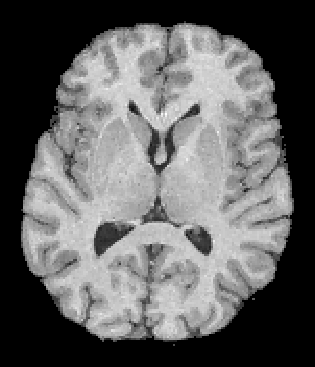
\includegraphics[width=\textwidth]{brain}
    \caption{}
    \label{fig:GMM_brain}
  \end{subfigure}
  \begin{subfigure}{0.94\textwidth}
    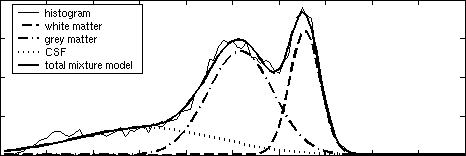
\includegraphics[width=\textwidth]{brainHistogram}
    \caption{}
    \label{fig:GMM_histogram}
  \end{subfigure}  
  \caption{In the Gaussian mixture model, the histogram is described as a linear superposition of Gaussian distributions: (\subref{fig:GMM_brain}) MR scan of the head, after removing all non-brain tissue and other pre-processing steps; and (\subref{fig:GMM_histogram}) corresponding histogram and its representation as a sum of Gaussians.}
  \label{fig:GMM}
\end{figure}


Because of the assumption of statistical independence between voxels, the segmentation posterior \eqref{eq:posterior} reduces to a simple form that is factorized (i.e., appears as a product) over the voxels:
\begin{eqnarray}
  p( \fat{l} | \fat{d}, \bldgr{\hat{\theta}}) & = & \frac{p( \fat{d} | \fat{l}, \bldgr{\hat{\theta}}_d ) p( \fat{l} | \bldgr{\hat{\theta}}_l )}%
                                                         {p( \fat{d} | \bldgr{\hat{\theta}} )} \nonumber\\
                                              & = & \frac{\prod_{n=1}^N \N( d_n | \hat{\mu}_{l_n}, \hat{\sigma}_{l_n}^2 ) \prod_{n=1}^N \hat{\pi}_{l_n}}%
                                                         {\prod_{n=1}^N \sum_{k=1}^K \N( d_n | \hat{\mu}_k, \hat{\sigma}_k^2 ) \hat{\pi}_k } \nonumber\\
                                              & = & \prod_{n=1}^N p( l_n | d_n, \bldgr{\hat{\theta}} ),
  \label{eq:GMMjointPosterior}
\end{eqnarray}
where 
\begin{equation}
  p( l=k | d, \bldgr{\hat{\theta}} ) = \frac{ \N( d | \hat{\mu}_k, \hat{\sigma}_k^2 ) \hat{\pi}_k }%
                                              { \sum_{k'=1}^K \N( d | \hat{\mu}_{k'}, \hat{\sigma}_{k'}^2 ) \hat{\pi}_{k'} }.
  \label{eq:GMMposterior}
\end{equation}
Therefore, the segmentation posterior is fully specified by each voxel's $K$ posterior probabilities of belonging to each structure; such segmentation posteriors can be visualized as images where high and low intensities correspond to high and low probabilities, respectively. The segmentation corresponding to the image and Gaussian mixture model of Fig.~\ref{fig:GMM} is visualized in~\ref{fig:GMMSegmentation} this way. 
Evidently, the sum of all the structures' posterior probabilities add to one in each voxel: $\sum_{k=1}^K p( l_n=k | d_n, \bldgr{\hat{\theta}} ) = 1, \forall n$. 

\begin{figure}
  \centering
  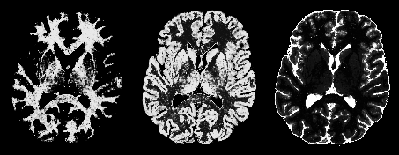
\includegraphics[width=0.96\textwidth]{brainTissueClassification}
  \caption{Visualization of the segmentation posterior corresponding to the data and model of Fig.~\ref{fig:GMM}. High intensities correspond to high probabilities and vice versa.}
  \label{fig:GMMSegmentation}
\end{figure}


Because of the factorized form of the segmentation posterior, the MAP segmentation \eqref{eq:MAP} is simply given by 
\begin{equation}
  \fat{\hat{l}} = \arg\max_{\fat{l}} p( \fat{l} | \fat{d}, \bldgr{\hat{\theta}}) = \arg \max_{l_1, \ldots, l_N} \prod_{n=1}^N p( l_n | d_n, \bldgr{\hat{\theta}} ),
\end{equation}
i.e., each voxel is assigned exclusively to the label with the highest posterior probability. Similarly, the expected volume of the anatomical structure corresponding to label $k$ is given by \eqref{eq:volume}
\begin{equation}
 \sum_{\fat{l}} V_k( \fat{l} )  p( \fat{l} | \fat{d}, \bldgr{\hat{\theta}} ) = \sum_{n=1}^N p( k | d_n, \bldgr{\hat{\theta}} ),
\end{equation}
i.e., a ``soft'' count of voxels belonging to the structure, where voxels contribute according to their posterior probability of belonging to that structure.


\section{Markov random field priors}

It is worth emphasizing that in the Gaussian mixture model, a voxel's posterior probability of belonging to each of the $K$ structures is computed using only the local intensity of the voxel itself (\eqref{eq:GMMposterior}). Although this works quite well in some applications, there is often an intensity overlap between the to-be-segmented structures, causing severe segmentation errors in such a purely intensity-driven strategy. An example of this is shown in Fig.~\ref{fig:tumor_noMRF}, where a simple Gaussian mixture model with $K=2$ classes was used to segment a brain MR scan into tumor tissue and other structures. The parameters $\bldgr{\hat{\theta}}$ were obtained by manually clicking on a set of representative voxels within the tumor, recording their intensities, and computing their mean and variance as estimates of $\hat{\mu}_1$ and $\hat{\sigma}_1^2$, respectively; the mean and variance $\{\hat{\mu}_2\, \hat{\sigma}_2^2\}$ for the ``other'' class was simply the mean and variance of all the image's voxels' intensities; and the tumor was estimated to cover approximately one tenth of the image area, so that we used $\hat{\pi}_1 = 0.1$ and $\hat{\pi}_2 = 0.9$. It can be seen from the figure that while this model generally captures the tumor quite well, many small image areas outside of the tumor also have a high posterior probability of belonging to the tumor class, limiting the usefulness of the results.

\begin{figure}
  \centering
  \begin{subfigure}{0.48\textwidth}
    \centering
    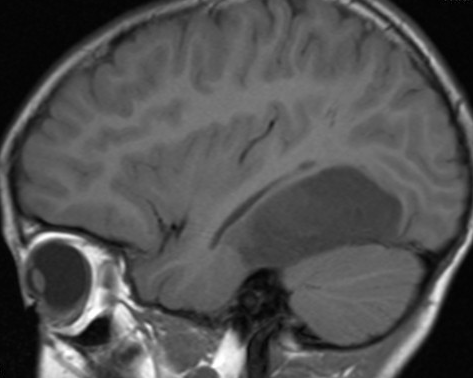
\includegraphics[width=\textwidth]{brainTumor}
    \caption{}
    \label{fig:tumor_noMRF_data}
  \end{subfigure}
  \begin{subfigure}{0.48\textwidth}
    \centering
    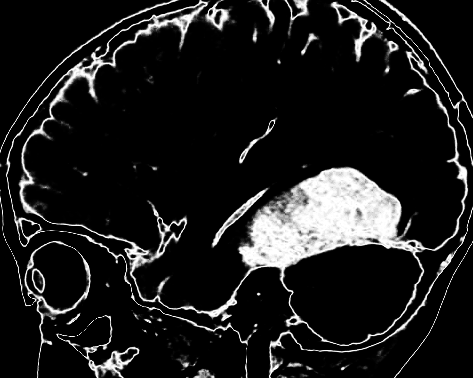
\includegraphics[width=\textwidth]{brainTumorSegmentation_noMRF}
    \caption{}
    \label{fig:tumor_noMRF_seg}
  \end{subfigure}  
  \caption{The Gaussian mixture model does not encode any spatial information and is therefore susceptible to segmentation errors caused by intensity overlap between the structures of interest: (\subref{fig:tumor_noMRF_data}) a brain MR scan of a person with a tumor; and (\subref{fig:tumor_noMRF_seg}) the voxels' posterior probability of belonging to the tumor for a 2-component Gaussian mixture model.}
  \label{fig:tumor_noMRF}
\end{figure}



In order to avoid this type of segmentation errors, we need to use more advanced models for the prior distribution $p(\fat{l} | \bldgr{\theta}_l )$ that more realistically reflect the shape of the structures we are looking for. 

\subsection{Markov random field model}

An often-used improvement to the simplistic prior of \eqref{eq:priorFrequency} is to use a prior that explicitly prefers voxels with the same label to be clustered spatially rather than scattered randomly throughout the image area. A computationally attractive way of achieving this is to formulate the prior as
\begin{equation}
  p( \fat{l} | \bldgr{\theta}_l ) = \frac{1}{Z( \bldgr{\theta}_l )} \exp( -U( \fat{l} | \bldgr{\theta}_l ) ),
  \label{eq:MRFGibbs}
\end{equation}
where $U(\fat{l} | \bldgr{\theta}_l )$ is an ``energy'' functional that is high for undesired configurations of $\fat{l}$ and low otherwise, resulting in low prior probabilities of undesired configurations and high probabilities otherwise. $Z(\bldgr{\theta}_l) = \sum_{\fat{l}} \exp( -U( \fat{l} | \bldgr{\theta}_l ) )$ is a normalizing constant that ensures that $\sum_{\fat{l}} p( \fat{l} | \bldgr{\theta}_l ) = 1$ but typically does not need to be computed explicitly in practical situations. 

For reasons that will soon become clear, the energy functional is often chosen to be of the form
% \begin{equation}
%   U( \fat{l} | \bldgr{\theta}_l ) = \frac{\beta}{2} \sum_{i} \sum_{j \in N_n} \delta( l_n, l_j ),
% \end{equation}
% where $N_n$ denotes the set of neighbors of voxel $n$ in the image grid (for instance, each voxel has six nearest neighbors in a 3-D image grid, or 26 if also the diagonal direction is allowed), $\delta( k, k' )$ is one if $k \neq k'$ and zero otherwise, and $\beta$ is a parameter that controls how strongly undesired configurations are penalized. 
\begin{equation}
  U( \fat{l} | \bldgr{\theta}_l ) = \beta \sum_{(n,n')} \delta( l_n \neq l_{n'} ),
\end{equation}
where the sum is running over all the voxel pairs $(n,n')$ that are neighbors in the image grid (for instance, each voxel has six direct neighbors in a 3-D image grid, or 26 if also the diagonal directions are allowed), $\delta( k \neq l )$ equals zero if $k = l$ and one otherwise, and $\beta$ is a parameter that controls how strongly undesired configurations are penalized. Stated differently, the energy functional is proportional to the number of times two neighboring voxels have a different class assignment in $\fat{l}$, thereby encouraging configurations in which the labels are spatially clustered.
Prior knowledge that some classes tend to occur more frequently than others can also be incorporated by adding an extra term:
\begin{equation}
  U( \fat{l} | \bldgr{\theta}_l ) = \beta \sum_{(n,n')} \delta( l_n \neq l_{n'} ) -\sum_{n=1}^N \log( \pi_{l_n} ).
  \label{eq:MRFcost}
\end{equation}
The parameters of this model are $\bldgr{\theta}_l = ( \beta, \pi_1, \ldots, \pi_K )\transp$; for $\beta=0$ (no undesired pair-wise combination penalized) this model reduces to the standard Gaussian mixture prior of \eqref{eq:priorFrequency}.

The computational attractiveness of the model lies in the fact that, although it defines a global prior that induces statistical dependencies between labels in voxels that are far apart, calculating the conditional distribution in a single voxel requires only looking up the labels assigned to its neighboring voxels (so-called Markov property). Indeed, using the notation $\fat{l}_{\setminus n} = ( l_1, \ldots, l_{n-1}, l_{n+1}, \ldots, l_n )\transp$ to denote the vector of labels in all voxels except voxel $n$, and $\mathfrak{N}_n$ the set of voxels that form neighboring pairs with voxel $n$, we have (Bayes' rule)
\begin{eqnarray}
  p( l_n | \fat{l}_{\setminus n} ) & = & \frac{ p( \fat{l} ) }{ p( \fat{l}_{\setminus n} ) } \nonumber\\
                                   & = & \frac{ p( \fat{l} ) }{ \sum_{l_n} p( \fat{l} ) } \nonumber\\
                                   & = & \frac{ \exp( -U(\fat{l} | \bldgr{\theta}_l) ) }{ \sum_{l_n} \exp( -U(\fat{l} | \bldgr{\theta}_l) ) }  \nonumber\\
                                   & = & \frac{ \exp\big( -\beta \sum_{{n'} \in \mathfrak{N}_n} \delta( l_{n'} \neq l_n ) +\log\pi_{l_n} \big) }%
                                              { \sum_{k=1}^K \exp\big( -\beta \sum_{n' \in \mathfrak{N}_n} \delta( l_{n'} \neq k ) +\log\pi_k \big)} \nonumber\\
                                   & = & \frac{ \pi_{l_n} \cdot \exp\big( -\beta \sum_{n' \in \mathfrak{N}_n} \delta( l_{n'} \neq l_n ) \big) }%
                                              { \sum_{k=1}^K \pi_k \cdot \exp\big( -\beta \sum_{n' \in \mathfrak{N}_n} \delta( l_{n'} \neq k ) \big)}.
  \label{eq:MRFconditional}                                
\end{eqnarray}
The second to last step is explained by the fact that all the remaining terms of \eqref{eq:MRFcost} cancel out in the numerator and the denominator.

Comparing \eqref{eq:MRFconditional} to the standard Gaussian mixture prior, the probability of having label $k$ in voxel $n$ is no longer simply $\pi_k$, but changes according to 
%how many neighboring voxels also have label $k$. 
the labels assigned to its neighboring voxels.
% 
% When there are $K=2$ possible labels, for instance, the probability of having $k$ in $n$ is higher than $\pi_k$ when the majority of the neighboring voxels also has label $k$
% 
% 
If the majority of neighbors has label $k$, for instance, the probability of having $k$ in $n$ will be higher than $\pi_k$.


\subsection{Inference using the mean-field approximation}
\label{sec:meanfield}

Combining the more advanced Markov random field prior with the same likelihood as before, in which the intensity in each voxel is distributed according to a Gaussian associated with its label (\eqref{eq:likelihood} and~\eqref{eq:Gauss}), we can in principle evaluate possible segmentations by comparing their posterior $p( \fat{l} | \fat{d}, \bldgr{\hat{\theta}} )$. However, handling this posterior explicitly is difficult in practice because it can no longer be written as a simple product of voxel-wise contributions in the same way as before (\eqref{eq:GMMjointPosterior}).%: each of the possible segmentations $\fat{l}$ has its own unique  

There exist fast algorithms, based on so-called graph-cuts, for computing the MAP segmentation $\fat{\hat{l}} = \arg\max_{\fat{l}} p( \fat{l} | \fat{d}, \bldgr{\hat{\theta}})$~\cite{graphCuts}. However, we are sometimes more interested in calculating \emph{expectations}, for instance in order to estimate volumes of anatomical structures (\eqref{eq:volume}) or as part of Expectation-Maximization parameter optimizers (which we will cover in Sec.~\ref{sec:EM}). Since this involves summing over all possible configurations of $\fat{l}$, it is infeasible to do the necessary computations exactly because there are exponentially many configurations of $\fat{l}$: a segmentation problem with just $K=2$ classes of a standard MR image of size $256\times256\times128$ voxels yields 
%
% 10^x = 2^(256*256*128) => x = 256*256*128 * log(2) / log( 10 )
more than 
% $10^{10^6}$ 
$10^{1000000}$
configurations to sum over\footnote{As a comparison, there are approximately $10^{80}$ atoms in the universe.}!

The solution is to resort to approximation schemes, of which one is a variational method based upon the so-called mean field theory in physics. In this method, we seek a distribution $q(\fat{l})$ that we design to be of a more tractable form than $p(\fat{l} | \fat{d}, \bldgr{\hat{\theta}})$, while still approximating $p(\fat{l} | \fat{d}, \bldgr{\hat{\theta}})$ as well as possible. One possibility is to impose the factorized form of the posterior of the standard Gaussian mixture model (\eqref{eq:GMMjointPosterior}) on $q(\fat{l})$, i.e., we chose $q(\fat{l})$ to be of the form
\begin{equation}
  q( \fat{l} ) = \prod_{n=1}^N q_n( l_n ).
  \label{eq:factorized}
\end{equation}
Within this family, our task is to chose the voxel-wise distributions $q_n(\cdot)$ in such a way that the resulting joint distribution $q(\fat{l})$ approximates $p(\fat{l} | \fat{d}, \bldgr{\hat{\theta}})$ as accurately as possible. For this purpose, we minimize the so-called Kullback-Leibler (KL) divergence
\begin{equation}
  {KL}\left( \, q( \fat{l} ) \, || \, p(\fat{l} | \fat{d}, \bldgr{\hat{\theta}}) \, \right) = - \sum_{\fat{l}} q( \fat{l} ) \log \frac{ p(\fat{l} | \fat{d}, \bldgr{\hat{\theta}}) }{ q( \fat{l} ) },
  \label{eq:KL}
\end{equation}
which measures how different $q( \fat{l} )$ is from $p(\fat{l} | \fat{d}, \bldgr{\hat{\theta}})$: it is always positive, and zero only if our approximation $q( \fat{l} )$ equals the true posterior $p(\fat{l} | \fat{d}, \bldgr{\hat{\theta}})$ exactly (which will typically be unattainable because we restrict the form of $q( \fat{l} )$ to \eqref{eq:factorized}).

For a given set of distributions $q_{n'}( \cdot )$ in all voxels $n' \neq n$, it can be shown~\cite{Jaakkola} that the remaining voxel's distribution $q_n( \cdot )$ that minimizes the KL-divergence is given by
\begin{equation}
  q_n( l_n=k ) = \frac{ \N( d_n | \hat{\mu}_k, \hat{\sigma}_k^2 ) \gamma_n(l_n=k) }%
                                              { \sum_{k'=1}^K \N( d_n | \hat{\mu}_{k'}, \hat{\sigma}_{k'}^2 ) \gamma_n( l_n=k' ) }
  \label{eq:meanfield}
\end{equation}
with
\begin{equation}
  \gamma_n( l_n = k) = 
  \frac{ \hat{\pi}_{k} \cdot \exp\big( -\beta \sum_{n' \in \mathfrak{N}_n} ( 1 - q_{n'}( l_{n'} = k ) ) \big) }%
       { \sum_{k'=1}^K \hat{\pi}_{k'} \cdot \exp\big( -\beta \sum_{n' \in \mathfrak{N}_n} ( 1 - q_{n'}( l_{n'} = k' ) ) \big) }.
  \label{eq:meanfieldPrior}
\end{equation}
Comparing this with the voxel-wise posterior of the standard Gaussian mixture model \eqref{eq:GMMposterior}, it can be seen that the usual class priors $\pi_k$ are replaced with altered priors $\gamma_n(k)$ that take the local neighborhood of the voxels into account: as in \eqref{eq:MRFconditional}, the number of neighboring voxels ``assigned'' to a different class is ``counted'' (in a soft, weighted sense) and alters $\pi_k$ accordingly.

Note that \eqref{eq:meanfield} gives the optimal distribution $q_n(k)$ for one voxel at a time, but that this result depends in turn on the result in other voxels. Therefore, a common strategy to minimize the KL-divergence is to cycle through the voxels in turn, updating each voxel's $q_n(k)$ based on the current result in the other voxels, and to continue this process until some convergence criterion is satisfied. With such a minimization strategy, the order in which the voxels are visited as well as the initialization of the $q_n(l_n)$'s may affect the local optimum of the KL divergence we arrive at.

% Jaakkola: The order in which the iterative updates are carried out as well as the initialization of the marginals affect which of the locally optimal solution we will arrive at.
A segmentation example on the tumor data of fig.~\ref{fig:tumor_noMRF} is shown in fig.~\ref{fig:tumor_MRF}, for different values of the Markov random field parameter $\beta$. It can be seen that the more advanced priors add contextual information that improves the segmentation results. 

\begin{figure}
  \centering
  \begin{subfigure}{0.48\textwidth}
    \centering
    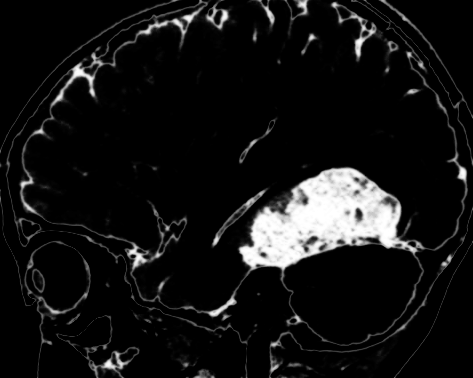
\includegraphics[width=\textwidth]{brainTumorSegmentation_withMRF_betaIsZeroDotTwentyFive}
    \caption{$\beta = 0.25$}
    \label{fig:tumor_MRF_segLowBeta}
  \end{subfigure}
  \begin{subfigure}{0.48\textwidth}
    \centering
    \includegraphics[width=\textwidth]{brainTumorSegmentation_withMRF_betaIsZeroDotFiftyFive}
    \caption{$\beta = 0.55$}
    \label{fig:tumor_MRF_segHighBeta}
  \end{subfigure}
  \caption{Visualization of the mean-field approximation to the segmentation posterior for the tumor data of Fig.~\ref{fig:tumor_noMRF}, for different settings of the Markov random field parameter $\beta$.}
  \label{fig:tumor_MRF}
\end{figure}


Once the voxel-wise distributions $q_n(l_n)$ have been computed, they can be used in the same way as the distributions $p( l_n | d_n, \bldgr{\hat{\theta}})$ to approximate expectations, e.g., the expected volume of the structure with label $k$ is approximately given by
\begin{equation}
 \sum_{\fat{l}} V_k( \fat{l} )  q(\fat{l}) = \sum_{n=1}^N q_n(l_n).
\end{equation}


\section{Parameter optimization using the EM algorithm}
\label{sec:EM}

So far we have assumed that appropriate values $\bldgr{\hat{\theta}}$ of our model parameters are known in advance.  
In the tumor segmentation example of the previous section, these parameters were estimated by manually clicking 
on some representative points in the image, and collecting statistics on the intensity of the selected voxels. In
general, however, such a strategy is impractical for such a versatile imaging modality as MRI, where intensities
do not directly correspond to any physical properties of the tissue being scanned. By merely tweaking the imaging protocol,
upgrading the scanner, or collecting images from different scanner models or manufacturers, the values of $\bldgr{\hat{\theta}}$
become inappropriate and need to be constructed again using manual interaction.

This difficulty can be avoided by estimating appropriate values for the model parameters automatically for each
individual scan, i.e., each scan receives its own, well-suited set of parameters that are computed without requiring any manual
interaction. This can be accomplished by estimating the parameters that maximize the so-called \emph{likelihood function} 
$p(\fat{d} | \bldgr{\theta})$, which expresses how probable the observed image $\fat{d}$ is for different settings of the parameter
vector $\bldgr{\theta}$:
\begin{eqnarray}
  \bldgr{\hat{\theta}} & = & \arg\max_{\bldgr{\theta}} \left[ p( \fat{d} | \bldgr{\theta} ) \right] \nonumber \\
                       & = & \arg\max_{\bldgr{\theta}} \left[ \log p( \fat{d} | \bldgr{\theta} ) \right] \label{eq:ML}.
\end{eqnarray}
The last step is true because the logarithm is a monotonically increasing function of its argument; it is used here because
maximizing the log likelihood function instead of the likelihood function directly simplifies the mathematical analysis considerably,
and also avoids numerical underflow problems in practical computer implementations.
The parameter vector $\bldgr{\hat{\theta}}$ resulting from \eqref{eq:ML} is commonly called the \emph{maximum likelihood} (ML) 
parameter estimate.

Maximizing the log likelihood function in image segmentation problems is a non-trivial optimization problem for which iterative 
numerical algorithms are needed. Although a variety of standard optimization methods could potentially be used, for the Gaussian mixture
model discussed in Sec.~\ref{sec:GMM} a dedicated and highly effective optimizer is available in the form of the so-called 
\emph{expectation-maximization} algorithm (EM)\footnote{For more complex models with Markov random field priors, an approximate 
EM algorithm is obtained by replacing the voxel-wise posteriors 
%$p(l_n | d_n, \bldgr{\hat{\theta}})$ 
with their mean-field approximations% $q_n(l_n)$
.}. The EM algorithm belongs to a family of optimization methods that work by repeatedly constructing
a lower bound to the objective function, maximizing that lower bound, and repeating the process until convergence~\cite{HunterAS2004}. 
This process is illustrated in Fig.~\ref{fig:lowerboundOptimization}. For a given starting estimate of the model parameters $\bldgr{ \tilde{\theta} }$,
a function of the model parameters $Q( \bldgr{\theta} | \bldgr{ \tilde{\theta} } )$ is constructed that equals the log likelihood 
function at $\bldgr{ \tilde{\theta} }$:
\begin{equation}
Q( \bldgr{\tilde{\theta}} | \bldgr{ \tilde{\theta} } ) = \log p( \fat{d} | \bldgr{ \tilde{\theta} } ),
\label{eq:lowerboundTouch}
\end{equation}
but that otherwise never exceeds it:
\begin{equation}
Q( \bldgr{\theta} | \bldgr{ \tilde{\theta} } ) \leq \log p( \fat{d} | \bldgr{ \theta} ),  \,\, \forall \bldgr{\theta}.
\label{eq:lowerbound}
\end{equation}
The parameter vector maximizing $Q( \bldgr{\theta} | \bldgr{ \tilde{\theta} } )$ is then computed and used as the new parameter
estimate $\bldgr{\tilde{\theta}}$, after which the whole process is repeated. Critically, because of \eqref{eq:lowerboundTouch} 
and~\eqref{eq:lowerbound}, updating the estimate $\bldgr{\tilde{\theta}}$ to the parameter vector that maximizes the lower bound 
automatically guarantees that the log likelihood function increases, by at least the same amount as the lower 
bound has increased. The consecutive estimates $\bldgr{\tilde{\theta}}$ obtained this way are therefore increasingly better estimates
of the maximum likelihood parameters -- one is \emph{guaranteed} to never move in the wrong direction in parameter space. This is a 
highly desirable property for a numerical optimization algorithm.


\begin{figure}
  \centering
  \begin{subfigure}{0.48\textwidth}
    \centering
    \includegraphics[width=\textwidth]{lowerBound1}
    \caption{}
    \label{fig:lowerboundOptimization_1}
  \end{subfigure}
  \hfill
  \begin{subfigure}{0.48\textwidth}
    \centering
    \includegraphics[width=\textwidth]{lowerBound2}
    \caption{}
    \label{fig:lowerboundOptimization_2}
  \end{subfigure}
  \begin{subfigure}{0.48\textwidth}
    \centering
    \includegraphics[width=\textwidth]{lowerBound3}
    \caption{}
    \label{fig:lowerboundOptimization_3}
  \end{subfigure}
  \hfill
  \begin{subfigure}{0.48\textwidth}
    \centering
    \includegraphics[width=\textwidth]{lowerBound4}
    \caption{}
    \label{fig:lowerboundOptimization_4}
  \end{subfigure}
  \begin{subfigure}{0.48\textwidth}
    \centering
    \includegraphics[width=\textwidth]{lowerBound5}
    \caption{}
    \label{fig:lowerboundOptimization_5}
  \end{subfigure}
  \hfill
  \begin{subfigure}{0.48\textwidth}
    \centering
    \includegraphics[width=\textwidth]{lowerBound6}
    \caption{}
    \label{fig:lowerboundOptimization_6}
  \end{subfigure}
  \caption{In the EM algorithm the maximum likelihood parameters $\bldgr{\hat{\theta}}$ are sought by repeatedly constructing a lower bound to the log likelihood function, in such a way that the lower bound touches the log likelihood function exactly at the current parameter estimate $\bldgr{\tilde{\theta}}$ (\subref{fig:lowerboundOptimization_1}). Subsequently the parameter estimate $\bldgr{\tilde{\theta}}$ is updated to the parameter vector that maximizes the lower bound (\subref{fig:lowerboundOptimization_2}). A new lower bound is then constructed at this new location (\subref{fig:lowerboundOptimization_3}) and maximized again (\subref{fig:lowerboundOptimization_4}), and so forth ((\subref{fig:lowerboundOptimization_5}) and (\subref{fig:lowerboundOptimization_6})), until convergence. In these plots, the log likelihood function is represented by a full line, and the successive lower bounds with a broken line.}
  \label{fig:lowerboundOptimization}
\end{figure}



While it is of course always possible to construct a lower bound to an objective function, nothing is gained if optimizing
the lower bound is not significantly easier and/or faster to perform than optimizing the objective function directly. However,
in the case of the Gaussian mixture model, it turns out it is possible to construct a lower bound for which the parameter vector 
maximizing it is given directly by analytical expressions. Therefore, the resulting algorithm effectively breaks up a difficult 
maximization problem (of the log likelihood function) into many smaller ones (of the lower bound) that are trivial to solve. Combined 
with the guarantee of increasingly better estimates of the maximum likelihood parameters as iterations progress, it should be clear
why this algorithm is a popular choice for maximum likelihood estimation of Gaussian mixture model parameters.

The trick exploited by the EM algorithm to construct its lower bound is based on the property of the logarithm that it is a \emph{concave} function, 
i.e., every chord connecting two points on its curve lies on or below that curve (see Fig.~\ref{fig:logConcave}). Mathematically, this means that
\begin{equation}
  \log \left[ w x_1 + ( 1- w ) x_2 \right ] 
  \,\, \geq \,\, 
  w \log x_1 + (1-w) \log x_2
  \nonumber
\end{equation}
for any two points $x_1$ and $x_2$ and $0 \leq w \leq 1$. 
It is trivial to show that this also
generalizes to more than two variables, (so-called \emph{Jensen's inequality}):
\begin{equation}
  \log( \sum_{k=1}^K w_k x_k ) \,\, \geq \,\, \sum_{k=1}^K w_k \log x_k
  \label{eq:Jensen}
\end{equation}
where $w_k \geq 0$ and $\sum_{k=1}^K w_k = 1$, for any set of points $\{ x_k \}$.
This can now be used to construct a lower bound to the likelihood function of the Gaussian mixture model as follows. 
Recalling that $p( \fat{d} | \bldgr{\theta} ) = \prod_{n=1}^N \left[ \sum_{k=1}^K \N( d_n | \mu_k, \sigma_k^2 ) \pi_k \right]$ (\eqref{eq:after} and~\eqref{eq:mixture}), we have
that
\begin{eqnarray}
  \log p( d | \bldgr{\theta} ) & = & \log \left(  \prod_{n=1}^N \left[ \sum_{k=1}^K \N( d_n | \mu_k, \sigma_k^2 ) \pi_k \right] \right) \\
                               & = & \sum_{n=1}^N \log \left[ \sum_{k=1}^K \N( d_n | \mu_k, \sigma_k^2 ) \pi_k \right] \\
                               & = &  \sum_{n=1}^N \log \left[ \sum_{k=1}^K \left( \frac{ \N( d_n | \mu_k, \sigma_k^2 ) \pi_k }{ \omega_{n,k} } \right) \omega_{n,k}  \right] \\
                               & \geq & \underbrace{ 
                                         \sum_{n=1}^N \left[ \sum_{k=1}^K \omega_{n,k}  \log \left( \frac{ \N( d_n | \mu_k, \sigma_k^2 ) \pi_k }{ \omega_{n,k} } \right) \right]
                                        }_{Q( \bldgr{\theta} | \bldgr{\tilde{\theta}} )},
                               \label{eq:EMLowerBound}
\end{eqnarray}
for any set of weights $\{\omega_{n,k}\}$ that satisfy $\omega_{n,k} \geq 0$ and $\sum_{k=1}^K \omega_{n,k} = 1$ (the last step relies on \eqref{eq:Jensen}). We now have a lower bound function $Q( \bldgr{\theta} | \bldgr{\tilde{\theta}} )$ that 
satisfies \eqref{eq:lowerbound}, but not \eqref{eq:lowerboundTouch}, so we are not done yet. Instead of randomly assigning \emph{any} valid $K$ weights $\omega_{n,k}$ to each voxel $n$ (one weight for each label $k$), we can satisfy \eqref{eq:lowerboundTouch} by choosing the weights so that
\begin{equation}
  \omega_{n,k} =  \frac{ \N( d_n | \tilde{\mu}_k, \tilde{\sigma}_k^2 ) \tilde{\pi}_k }%
                { \sum_{k'=1}^K \N( d_n | \tilde{\mu}_{k'}, \tilde{\sigma}_{k'}^2 ) \tilde{\pi}_{k'} }.
  \label{eq:EMWeights}
\end{equation}
By filling these weights into the definition of our lower bound \eqref{eq:EMLowerBound}, it is easy to check that \eqref{eq:lowerboundTouch} is indeed fulfilled with this choice.

\begin{figure}
  \centering
  \includegraphics[width=0.98\textwidth]{Jensen}
  \caption{Because the logarithm is a concave function, the cord between any two points on its curve lies on or below the curve. An example cord is shown in blue.}
  \label{fig:logConcave}
\end{figure}

Setting the new model parameter estimate $\bldgr{\tilde{\theta}}$ to the parameter vector that maximizes the lower bound requires finding the location where
\begin{displaymath}
  \frac{\partial Q( \bldgr{\theta} | \bldgr{\tilde{\theta}} )}{ \partial \bldgr{\theta}} = 0.
\end{displaymath}
Reformulating the lower bound as
\begin{eqnarray}
  Q( \bldgr{\theta} | \bldgr{\tilde{\theta}}) & = & -\frac{1}{2} \sum_{k=1}^K \left[ \frac{1}{\sigma_k^2}\sum_{n=1}^N \omega_{n,k} \left( d_n - \mu_k  \right)^2  
                                                                               + \left( \sum_{n=1}^N \omega_{n,k}  \right) \log \sigma_k^2 \right] 
                                                    \nonumber \\ 
                                              & &  + \sum_{k=1}^K \left[ \left( \sum_{n=1}^N \omega_{n,k} \right) \log \pi_k \right] \nonumber \\
                                              & &  - \sum_{n=1}^N\sum_{k=1}^K \omega_{n,k} \log \omega_{n,k} -\frac{N}{2}\log\left( 2 \pi \right),
  \label{eq:EMLowerBoundReformulated}
\end{eqnarray}
it is straightforward to show that the parameter updates 
%that maximize it 
are given by
\begin{eqnarray}
  \tilde{\mu}_k & \gets & \frac{\sum_{n=1}^N \omega_{n,k} d_n}{\sum_{n=1}^N \omega_{n,k}} \nonumber \\ 
  \tilde{\sigma}_k^2 & \gets & \frac{\sum_{n=1}^N \omega_{n,k} \left( d_n - \tilde{\mu}_k \right)^2 }{\sum_{n=1}^N \omega_{n,k}} \label{eq:EMUpdateRules}\\ 
  \tilde{\pi}_k & \gets & \frac{\sum_{n=1}^N \omega_{n,k} }{N}. \nonumber
\end{eqnarray}

It is worth spending some time thinking about these equations. The EM algorithm searches for the maximum likelihood parameters of the Gaussian mixture model merely be repeatedly applying the update rules of \eqref{eq:EMUpdateRules}, where the weights $\omega_{n,k}$ are defined in \eqref{eq:EMWeights}. These weights depend themselves on the current estimate of the model parameters, which explains why the algorithm involves iterating. More importantly, by comparing \eqref{eq:EMWeights} to \eqref{eq:GMMposterior}, we see that these weights represent nothing but the posterior probability of the segmentation, given the current model parameter estimate! Thus, the EM algorithm repeatedly computes the type of probabilistic segmentation shown in Fig.~\ref{fig:GMMSegmentation} based on its current parameter estimate, and then updates the parameter estimate accordingly. The update rules of \eqref{eq:EMUpdateRules} are remarkably intuitive: the mean and variance of the Gaussian distribution associated with the $k$th label are simply set to the weighted mean and variance of the intensities of those voxels currently attributed to that label; similarly the prior for each class is set to the fraction of voxels currently attributed to that class.

Fig.~\ref{fig:EMProgress} shows a few iterations of the EM algorithm searching for the maximum likelihood parameters of the brain MR data shown in Fig.~\ref{fig:GMM_brain}.

\begin{figure}
  \centering
  \begin{subfigure}{0.48\textwidth}
    \centering
    \includegraphics[width=\textwidth]{croppedFrame01}
    \caption{Initialization}
  \end{subfigure}
  \hfill
  \begin{subfigure}{0.48\textwidth}
    \centering
    \includegraphics[width=\textwidth]{croppedFrame02}
    \caption{After one iteration}
  \end{subfigure}
  \begin{subfigure}{0.48\textwidth}
    \centering
    \includegraphics[width=\textwidth]{croppedFrame11}
    \caption{After 11 iterations}
  \end{subfigure}
  \hfill
  \begin{subfigure}{0.48\textwidth}
    \centering
    \includegraphics[width=\textwidth]{croppedFrame30}
    \caption{After 30 iterations}
  \end{subfigure}
  \caption{Iterative improvement of the Gaussian mixture model parameters for the MR image of Fig.~\ref{fig:GMM_brain}, using the EM algorithm.}
  \label{fig:EMProgress}
\end{figure}


\section{Modeling MR bias fields}
\label{sec:biasField}

Although the Gaussian mixture model is a very useful tool for image segmentation, and comes with a an dedicated parameter estimation algorithm, 
it can often not be applied directly to MR images. This is because MR suffers from an imaging artifact that makes some image areas darker and other
areas brighter than they should be. This spatially smooth variation of intensities is often referred to
as MR ``intensity inhomogeneity'' or ``bias field'', and is caused by imaging equipment limitations and electrodynamic interactions with the object
being scanned. Interestingly, the bias field artifact is dependent on the anatomy being imaged and therefore unique to each scan session, and is
much more pronounced in the newest generation of scanners (see Fig.~\ref{fig:biasField}).

\begin{figure}
  \centering
  \begin{subfigure}[t]{0.33\textwidth}
    \centering
    \includegraphics[height=\textwidth]{biasField1pt5T}
    \caption{1.5 Tesla}
  \end{subfigure}
  \hspace{-1ex}
  \begin{subfigure}[t]{0.33\textwidth}
    \centering
    \includegraphics[height=\textwidth]{biasField3T}
    \caption{3 Tesla}
  \end{subfigure}
  \hspace{-1ex}
  \begin{subfigure}[t]{0.33\textwidth}
    \centering
    \includegraphics[height=\textwidth]{biasField7T}
    \caption{7 Tesla}
  \end{subfigure}
  \caption{The MR bias field artifact is often more pronounced in scanners operating at higher magnetic field strengths.}
  \label{fig:biasField}
\end{figure}


Since the Gaussian mixture model does not account for smoothly varying overall intensity levels within one and the same anatomical structure, it is 
very susceptible to segmentation errors when applied to typical MR data. However, this problem can be avoided
by explicitly taking a model for the bias field artifact into account in the imaging component of the generative model. In particular, we can model
the artifact as a linear combination of $M$ spatially smooth basis functions
\begin{equation}
  \sum_{m=0}^{M-1} c_m \phi_{n,m},
  %\label{eq:linearBasisFunctions}
\end{equation}
where $\phi_{n,m}$ is shorthand for $\phi_m( \fat{x}_n )$, the value of the $m$th basis function evaluated at voxel $n$, which has spatial location $\fat{x}_n$.
Suitable basis functions can be 2D DCT basis functions, 2D B-spline basis functions (such as those shown in Fig.~\ref{fig:basisFunctions2D_BSpline}), or something similar.
We can then extend the imaging model of the Gaussian mixture model by still assigning each voxel an intensity drawn from a Gaussian distribution
associated with its label, but further \emph{adding}\footnote{Because of the physics of MR, the bias field is better modeled as a multiplicative rather than an additive artifact. This can be taken into account by working with logarithmically transformed intensities in the models, instead of using directly the original MR intensities.} the bias model to the resulting intensity image to obtain the final, bias field corrupted image $\fat{d}$.  With this model, we have
\begin{equation}
  p( \fat{d} | \fat{l}, \bldgr{\theta}_d ) = \prod_{n=1}^N \N \!\, \Big( d_n \,\, \Big| \mu_{l_n} + \sum_{m-1}^M c_m \phi_{n,m}, \,\, \sigma_{l_n}^2 \Big) 
\end{equation}
with parameters $\bldgr{\theta}_d = ( \mu_1, \ldots, \mu_K, \sigma_1^2, \ldots, \sigma_K^2, c_0, \ldots, c_{M-1})\transp$, which consist not only of the parameters associated with the Gaussian distributions, but additionally also the $M$ coefficients of the bias field basis functions, $c_m$. 

As was the case with the Gaussian mixture model, model parameter estimation can be performed conveniently by iteratively constructing a lower bound to the log likelihood function% of the parameters
, and working with that lower bound instead. For constructing the lower bound in this case, we follow the exact same procedure as in the previous section to obtain
\begin{eqnarray}
  Q( \bldgr{\theta} | \bldgr{\tilde{\theta}}) & = & -\frac{1}{2} \sum_{k=1}^K \left[ \frac{1}{\sigma_k^2}\sum_{n=1}^N \omega_{n,k} \left( d_n - \mu_k - \sum_{m-1}^M c_m \phi_{n,m} \right)^2  
                                                                               + \left( \sum_{n=1}^N \omega_{n,k}  \right) \log \sigma_k^2 \right] 
                                                    \nonumber \\ 
                                              & &  + \sum_{k=1}^K \left[ \left( \sum_{n=1}^N \omega_{n,k} \right) \log \pi_k \right] \nonumber \\
                                              & &  - \sum_{n=1}^N\sum_{k=1}^K \omega_{n,k} \log \omega_{n,k} -\frac{N}{2}\log\left( 2 \pi \right),
  \label{eq:GEMLowerBound}
\end{eqnarray}
where now the weights satisfying \eqref{eq:lowerboundTouch} are given by
\begin{equation}
  \omega_{n,k} =  \frac{ \N \!\, \Big( d_n \,\, \Big| \tilde{\mu}_k + \sum_{m-1}^M \tilde{c}_m \phi_{n,m}, \,\, \tilde{\sigma}_k^2 \Big) \tilde{\pi}_k }%
                { \sum_{k'} \N \!\, \Big( d_n  \,\, \Big| \tilde{\mu}_{k'} + \sum_{m-1}^M \tilde{c}_m \phi_{n,m}, \,\, \tilde{\sigma}_{k'}^2 \Big) \tilde{\pi}_{k'}  }.
  \label{eq:GEMWeights}
\end{equation}
Maximizing this lower bound is more complicated than in the Gaussian mixture model, however, because setting the derivative with respect to the parameter vector 
$\bldgr{\theta}$ to zero no longer yields analytical expressions for the parameter update rules. 
If we keep the bias field parameters fixed at their current values $\tilde{c}_m$, and only maximize the lower bound with respect to the Gaussian mixture model parameters, we easily
obtain
\begin{eqnarray}
  \tilde{\mu}_k & \gets & \frac{\sum_{n=1}^N \omega_{n,k} \left( d_n - \sum_{m-1}^M \tilde{c}_m \phi_{n,m} \right) }{\sum_{n=1}^N \omega_{n,k}} \nonumber \\ 
  \tilde{\sigma}_k^2 & \gets & \frac{\sum_{n=1}^N \omega_{n,k} \left( d_n - \sum_{m-1}^M \tilde{c}_m \phi_{n,m}- \tilde{\mu}_k \right)^2 }{\sum_{n=1}^N \omega_{n,k}} \label{eq:GEMUpdateRulesGMMParameters}\\ 
  \tilde{\pi}_k & \gets & \frac{\sum_{n=1}^N \omega_{n,k} }{N}. \nonumber
\end{eqnarray}
Similarly, keeping the Gaussian mixture model parameters fixed at their current values, it is easy to see that the bias field parameters maximizing the lower bound are given in analytical form as well: the lower bound is a quadratic function of the coefficients $c_m$, and finding their optimal values is therefore merely a linear basis function regression problem (see Sec.~\ref{sec:linearRegression}). In particular, the solution is given by
\begin{equation}
  \tilde{\fat{c}} \,\, \gets \,\, ( \bldgr{\Phi}\transp \fat{P} \bldgr{\Phi} )^{-1} \bldgr{\Phi}\transp \fat{P} \fat{r}
  \label{eq:GEMUpdateRulesBiasFieldParameters}
\end{equation}
where 
$\bldgr{\Phi}$ is given by~\eqref{eq:Phi}
and
\begin{eqnarray*}
p_{n,k} =
\frac{ \omega_{n,k} }{\tilde{\sigma}_k^2}, 
\quad
p_n = \sum_{k=1}^K p_{n,k},
\quad
\fat{P} = \mbox{diag}(p_1, \ldots, p_N), 
\\
\tilde{d}_n = \frac{\sum_{k=1}^K p_{n,k} \tilde{\mu}_k}{\sum_{k=1}^K p_{n,k} },
\quad
\bldgr{r} =
\left(
\begin{array}{@{}c@{}}
   d_1 - \tilde{d}_1\\
   \vdots \\
   d_N - \tilde{d}_N
\end{array}
\right).
\end{eqnarray*}

Since \eqref{eq:GEMUpdateRulesGMMParameters} and \eqref{eq:GEMUpdateRulesBiasFieldParameters} depend on one another, one could
in principle try to maximize the lower bound by cycling through these two equations, one at a time, until some convergence criterion is met.
However, the desirable property of the EM algorithm to never decrease the value of the likelihood function with each new iteration
still holds even when the lower bound is not \emph{maximized} but merely \emph{improved}. Therefore, a more efficient strategy is to 
construct the lower bound by computing the weights $\omega_{n,k}$ (\eqref{eq:GEMWeights}) and then 
update the Gaussian mixture model parameters (\eqref{eq:GEMUpdateRulesGMMParameters}) and subsequently the bias field parameters 
(\eqref{eq:GEMUpdateRulesBiasFieldParameters})  only \emph{once} to merely improve it. After that a new lower bound is
constructed by recomputing the weights, which is again improved by updating the model parameters, etc, until convergence. 
Such an optimization strategy of only partially optimizing the EM lower bound is known as so-called
\emph{generalized expectation-maximization}.

The interpretation of the update equations is again very intuitive. As was the case in the Gaussian mixture model, the weights $\omega_{n,k}$
represent again a statistical classification of the image voxels as in Fig.~\ref{fig:GMMSegmentation}, and the mixture model parameters
are again updated accordingly. The only difference now is that instead of the original MR intensities, $d_n$, the bias field corrected
intensities, $d_n - \sum_{m-1}^M \tilde{c}_m \phi_{n,m}$, i.e., the intensities after the estimated bias field has been subtracted, are used.
Regarding the bias field update, the algorithm tries to make a reconstruction $(\tilde{d}_1, \ldots, \tilde{d}_N)\transp$ of what 
the image should look without the bias field artifact (shown in Fig.~\ref{fig:biasFieldEquationIllustration_b}), 
subtracts that from the MR scan to obtain a (noisy) estimate of the bias field (image $\fat{r}$, shown in Fig.~\ref{fig:biasFieldEquationIllustration_c}), 
and smoothes the result to obtain an estimate of the bias field
(shown in Fig.~\ref{fig:biasFieldEquationIllustration_e}). For the smoothing, each voxel has a weight $p_n$ 
(shown in Fig.~\ref{fig:biasFieldEquationIllustration_d}) that depends on the variance of the class it is attributed
to, reflecting the confidence in the local value of $\fat{r}$ (classes with tighter variances are more trustable than
classes with very large variances).

\begin{figure}
  \centering
  \begin{subfigure}[t]{0.3\textwidth}
    \centering
    \includegraphics[width=\textwidth]{biasFieldEstimationData}
    \caption{MR scan} 
  \end{subfigure}
  \hfill
  \begin{subfigure}[t]{0.3\textwidth}
    \centering
    \includegraphics[width=\textwidth]{biasFieldEstimationReconstruction}
    \caption{Reconstruction}
    \label{fig:biasFieldEquationIllustration_b}
  \end{subfigure}
  \hfill
  \begin{subfigure}[t]{0.3\textwidth}
    \centering
    \includegraphics[width=\textwidth]{biasFieldEstimationResidue}
    \caption{Difference between the MR scan and the reconstruction} 
    \label{fig:biasFieldEquationIllustration_c}
  \end{subfigure}
  \begin{subfigure}{0.3\textwidth}
    \centering
    \includegraphics[width=\textwidth]{biasFieldEstimationWeights}
    \caption{Weight image} 
    \label{fig:biasFieldEquationIllustration_d}
  \end{subfigure}
  \hspace{2ex}
  \begin{subfigure}{0.3\textwidth}
    \centering
    \includegraphics[width=\textwidth]{biasFieldEstimationEstimatedBiasField}
    \caption{Estimated bias field} 
    \label{fig:biasFieldEquationIllustration_e}
  \end{subfigure}
  \caption{Illustration of the bias field estimation within a generalized expectation-maximization algorithm.}
  \label{fig:biasFieldEquationIllustration}
\end{figure}


% By extending the Gaussian mixture model with an explicit model for the bias field artifact, it is possible to obtain high-quality 
% segmentations of MR scans without need . An example of this is shown in Fig.~\ref{fig:biasFieldEstimation}, 
% where a brain tissue classification result is shown both with and without taking the bias field model into account.
By extending the Gaussian mixture model with an explicit model for the bias field artifact this way, it is possible to obtain high-quality 
segmentations of MR scans without errors caused by intensity inhomogeneities, as shown in Fig.~\ref{fig:biasFieldEstimation}.

\begin{figure}
  \centering
  \begin{subfigure}{0.95\textwidth}
    \centering
    \includegraphics[width=\textwidth]{tmi1Fig4_stripped_Part-0}
    \caption{}
    \label{fig:biasFieldEstimation_part0}
  \end{subfigure}
  \begin{subfigure}{0.95\textwidth}
    \centering
    \includegraphics[width=\textwidth]{tmi1Fig4_stripped_Part-1}
    \caption{}
    \label{fig:biasFieldEstimation_part1}
  \end{subfigure}
  \begin{subfigure}{0.95\textwidth}
    \centering
    \includegraphics[width=\textwidth]{tmi1Fig4_stripped_Part-2}
    \caption{}
    \label{fig:biasFieldEstimation_part2}
  \end{subfigure}
  \begin{subfigure}{0.95\textwidth}
    \centering
    \includegraphics[width=\textwidth]{tmi1Fig4_stripped_Part-3}
    \caption{}
    \label{fig:biasFieldEstimation_part3}
  \end{subfigure}
  \caption{Explicitly modeling and estimating the bias field artifact in MR scans often improves segmentation results considerably. Shown are a few sagittal slices from a brain MR scan (\subref{fig:biasFieldEstimation_part0}); the posterior probability for white matter using the standard Gaussian mixture model (\subref{fig:biasFieldEstimation_part1}); the same when a bias field model is explicitly taken into account (\subref{fig:biasFieldEstimation_part2}); and the automatically estimated bias field model (\subref{fig:biasFieldEstimation_part3}). Note the marked improvement in segmentation accuracy in the upper parts of the brain.}
  \label{fig:biasFieldEstimation}
\end{figure}





\fi

\if\hideChapterNeuralNetworks0

\chapter{Neural Networks}
\label{chap:neuralNetworks}


The methods for registration and segmentation that we have seen so far are all based on \emph{models}
that 
%implictly or explicitly 
%to various degrees
somehow
encode prior knowledge of the problem at hand.
% somehow [implictly or explicitly]
% describe properties 
% express 
% incorporate our prior knowledge of the problem, such as that 
For instance,
mutual information-based registration 
%relies on 
%expresses the observation
%uses 
exploits
the fact
that one image is predictive of another image
only 
when the two are well aligned;
while the Gaussian mixture model for segmentation 
encodes the knowledge that voxels with the same label typically have similar intensities.
%

%
% Another approach is to make do with models, and learn instead.
% Advantage: simple, fast to apply
% Disadvantage: training data is sparse in medical imaging, domain shift (contrast with computer vision)
% Used in registration, segmentation, prediction, but here (voxel-based) segmentation.
% 
A completely different approach to solving a problem is not to try to understand 
%and model 
it, 
but rather to simply emulate successful example solutions. 
As opposed to the generative models of Chapter~\ref{chap:modelBasedSegmentation},
this approach to model-free ``machine learning'' is called \emph{discriminative} learning.
In this chapter we will review a specific class of discriminative methods based on artificial neural networks.
Although such networks can also be used for other purposes, such as image registration and computer aided diagnosis,
they are especially successful in the area of image segmentation, 
%and we will concentrate on that application 
which we will focus on
in this chapter.


In general, it should be noted that sidestepping the difficulty of building models is both the main strength and the most important weakness of 
%these methods. 
neural networks.
As long as sufficient example solutions are available, they are 
%much easier to deploy 
very easy to deploy without requiring any domain-specific knowledge, and can be orders of magnitude faster than model-based methods. 
On the other hand, however, example solutions are often in short supply in medical image analysis, as manually annotating a large set of images can be excruciatingly time consuming. Especially in versatile imaging modalities such as MRI, this problem is exacerbated by the differences in scanning hardware, software and protocols that exist 
%across clinical sites, 
even within 
%one clinical site,
the same hospital,
which can make 
%existing 
carefully curated
example solutions useless overnight.



\section{Logistic regression}
\label{sec:logisticRegression}

In Chapter~\ref{chap:modelBasedSegmentation} we saw how the Gaussian mixture model can be used to classify each image voxel into one of $K$ different classes (tissue types) based on its intensity alone. Specifically, we modeled the prior probability of a  voxel belonging to class 
%$k \in {1, \ldots, K}$ 
$k$
as 
$\pi_k$, 
and the intensity distribution associated with class $k$ as a Gaussian with mean $\mu_k$ and variance $\sigma_k^2$.
Using Bayes' rule, we then 
%\emph{indirectly} 
obtained the 
%posterior distribution 
probability
of a voxel having label $l$ 
%based on its intensity $d$
as
(cf.~(\eqref{eq:GMMposterior}))
\begin{equation}
  p( l = k | d, \bldgr{\theta} ) = \frac{ \N( d | \mu_k, \sigma_k^2 ) \pi_k }%
                                              { \sum_{k'} \N( d | \mu_{k'}, \sigma_{k'}^2 ) \pi_{k'} },  
\end{equation}
where 
$d$ is the voxel's intensity and 
$\bldgr{\theta}$ are the parameters of the model (collecting $\pi_k$, $\mu_k$ and $\sigma_k^2$ for all classes).

Rather than 
%modeling [\emph{indirectly}] [trying to model] the generative process,
using such models,
another way of obtaining a voxel-wise classifier $p( l | d, \bldgr{\theta} )$ 
is by 
%interpolating between 
%[ \emph{directly} 
simply mimicking the 
behavior
seen in
(``learning from'') examples.
%In particular, using the same notation as that for regression in Chapter~\ref{chap:fitting}, imagine we are given a training set of observed inputs and outputs, i.e., $\{\fat{x}_n, y_n\}_{i=1}^N$, where $\fat{x}_n =(x_{i1},x_{i2},\ldots,x_{ip})\transp$ is the vector of observed inputs for the $n$th case, and $y_n$ the corresponding output.
For reasons that will soon become clear, 
for the remainder of this chapter
we will switch to the notation used for regression in Chapter~\ref{chap:smoothingAndInterpolation},
indicating a training set of observed example inputs and outputs as $\{\fat{x}_n, t_n\}_{n=1}^N$, where $\fat{x}_n$ is the $D$-dimensional vector of observed inputs for the $n$th case, and $t_n$ the corresponding output.
For voxel-wise classification, 
%the input dimensionality is $p=1$, i.e., $\fat{x}_n = d_n$
each input is simply an intensity
$\fat{x}_n = d_n$, 
i.e., the input dimensionality is $D=1$,
but we will soon see cases where $\fat{x}_n$ is 
%a vector collecting intensities of several neighboring voxels simultaneously.
higher-dimensional.
Unlike in the regression case, where each output $t_n$ was a continuous value, 
for classification the outputs can only take 
$K$
discrete values, indicating which class 
%the $n$th 
each
example belongs to.
To simplify notation, here we only consider scenarios with $K=2$ classes\footnote{The generalization to several classes is rather straightforward (cf.~\cite{bishop2006pattern}, chapter 4).}.
%The output $y_n \in \{0,1\}$ can then be taken to be a binary value, 
The outputs can then be denoted as taking binary values $t_n \in \{0,1\}$, 
where 
%$y_n=1$ if $l_k=1$, and $y_n=0$ if $l_k=2$.
values $1$ and $0$ 
%indicate that 
correspond to the class assignments
$l_n=1$ and $l_n=2$, respectively.


%To model $p( l | d, \bldgr{\theta} )$ -- or, using the equivalent notation, $p( y | \fat{x}, \bldgr{\theta} )$ --
To model $p( y | \fat{x}, \bldgr{\theta} )$
-- which is equivalent to modeling $p( l | d, \bldgr{\theta} )$ in our 
voxel-wise classification
example -- 
we start from a parametric curve of the form 
\begin{equation}
  f( \fat{x} ) = \sigma\left( \sum_{m=0}^{M-1} w_m \phi_m( \fat{x} ) \right),
  \label{eq:logisticRegression}
\end{equation}
which is similar to the linear basis function model for regression we saw in Sec.~\ref{sec:linearRegression}:
%(cf.~(\eqref{eq:linearBasisFunctions})):
%Each $\phi_m(\fat{x}), m=1,\ldots,M$ is a nonlinear \emph{basis function} with a tunable coefficient $\beta_m$,
A linear combination of $M$ nonlinear basis functions $\phi_m(\fat{x})$ with tunable coefficients $w_m$,
which we here collect in the parameter vector $\bldgr{\theta} = (w_0,\ldots,w_{M-1})\transp$.
Unlike in the regression case, however, 
where the 
%linear combination 
%of basis functions 
quantity
\begin{equation}
  a = \sum_{m=0}^{M-1} w_m \phi_m( \fat{x} )
  \label{eq:activation}
\end{equation}
was used directly,
%(cf.~(\eqref{eq:linearBasisFunctions})),
here it is subject to a ``squashing'' function 
(illustrated in Fig.~\ref{fig:squashFunction})
\begin{equation}
  \sigma( a ) = \frac{1}{1 + \exp(-a)}
  \label{eq:squashFunction}
\end{equation}
that maps the result into the interval $[ 0, 1 ]$.
%
Because of this mapping, $f(\fat{x})$ can be interpreted as a probability:
$
  p( t=1 | \fat{x}, \bldgr{\theta} ) = f( \fat{x} )
  .
$
Since 
%conversely
$
  p( t=0 | \fat{x}, \bldgr{\theta} ) 
  = 1 - p( t=1 | \fat{x}, \bldgr{\theta} )
  = 1 - f( \fat{x} )
  ,
$
we can then write (Bernoulli distribution):
\begin{equation}
  p( t | \fat{x}, \bldgr{\theta} ) = f( \fat{x} )^t [ 1 - f( \fat{x} ) ]^{1-t}
  \label{eq:Bernoulli}
  .
\end{equation}
Because the mapping function $\sigma(a)$ in (\eqref{eq:squashFunction}) is called the ``logistic function'',
the model of (\eqref{eq:logisticRegression}) is known as ``logistic regression''.

\begin{figure}
  \centering
  \includegraphics[width=0.55\textwidth]{logisticFunction} 
  \caption{The logistic function $\sigma(a)$ defined in (\eqref{eq:squashFunction}) maps the domain $[ -\infty, \infty]$ into $[ 0, 1 ]$.}
  \label{fig:squashFunction}
\end{figure}


Given our training set 
%$\{\fat{x}_n, y_n\}_{i=1}^N$, 
of $N$ 
%independent 
input observations $\fat{X} = \{\fat{x}_1, \ldots, \fat{x}_N \}$
with corresponding outputs  $\fat{t} = \{ t_1, \ldots, y_N \}$,
appropriate values for the model parameters $\bldgr{\hat{\theta}}$ can be found by numerically
maximizing the likelihood function
\begin{equation}
  p( \fat{t} | \fat{X}, \bldgr{\theta} ) = \prod_{n=1}^N p( t_n | \fat{x}_n, \bldgr{\theta} )
  \label{eq:NNLikelihood}
\end{equation}
with respect to $\bldgr{\theta}$.
Once fitted this way,
%The fitted 
the
model can subsequently be used to classify new voxels simply by evaluating  
$$
  p( l=1 | d, \bldgr{\hat{\theta}} ) = 
  p( t=1 | \fat{x}, \bldgr{\hat{\theta}} )
  = \sigma\left( \sum_{m=0}^{M-1} \hat{w}_m \phi_m( \fat{x} ) \right)
  ,
$$
and assigning a voxel to class $1$ if $p( l=1 | d, \bldgr{\hat{\theta}} ) > 0.5$
and to class $2$ otherwise.

%
Fig.~\ref{fig:logisticRegressionImageClassification} illustrates this procedure on an MRI scan of the kidneys,
using the five 1D cosines of Fig.~\ref{fig:basisFunctions1D_DCT} as basis functions $\phi_m( \fat{x} )$ and $N=50$ training points.


\begin{figure}
  \centering
  \begin{subfigure}{0.3\textwidth}
    \centering
    \includegraphics[width=\textwidth]{scenario1_training_sampleLocations}
    \caption{}
    \label{fig:logisticRegressionImageClassification_a}
  \end{subfigure}
  \begin{subfigure}{0.3\textwidth}
    \centering
    \includegraphics[width=\textwidth]{scenario1_training_posteriorImage}
    \caption{}
    \label{fig:logisticRegressionImageClassification_b}
  \end{subfigure}
  \begin{subfigure}{0.3\textwidth}
    \centering
    \includegraphics[width=\textwidth]{scenario1_finalSegmentationOverlay}
    \caption{}
    \label{fig:logisticRegressionImageClassification_c}
  \end{subfigure}
  %
  %
  \begin{subfigure}{0.35\textwidth}
    \centering
    \includegraphics[width=\textwidth]{scenario1_training_activation}
    \caption{}
    \label{fig:logisticRegressionImageClassification_d}
  \end{subfigure}
  \begin{subfigure}{0.35\textwidth}
    \centering
    \includegraphics[width=\textwidth]{scenario1_training_posteriors}
    \caption{}
    \label{fig:logisticRegressionImageClassification_e}
  \end{subfigure}
  \caption{Example of a logistic regression classifier trained to discern pixels in the inner organs from pixels in other areas.
  (\subref{fig:logisticRegressionImageClassification_a}) Image to be segmented, along with training data consisting of 25 manually selected points inside ($l=1$, blue circles) and 25 points outside ($l=2$, red crosses) the area of interest. 
  (\subref{fig:logisticRegressionImageClassification_b}) The output $p( l=1 | d, \bldgr{\hat{\theta}} )$ of the trained classifier, evaluated in each pixel.
  (\subref{fig:logisticRegressionImageClassification_c}) Final segmentation produced by the trained classifier, overlaid on top of the input image.
  (\subref{fig:logisticRegressionImageClassification_d}) The quantity $a$ of (\eqref{eq:activation}) for various intensity levels $d$.
  (\subref{fig:logisticRegressionImageClassification_e}) The classifier resulting from subjecting $a$ to the squashing function $\sigma(a)$ of (\eqref{eq:squashFunction}). For reference, the intensity levels and labels of the 50 training points are also shown.
  }
  \label{fig:logisticRegressionImageClassification}
\end{figure}




\section{Training with stochastic gradient descent}

So far we have not specified how to 
%find  $\bldgr{\hat{\theta}}$ 
numerically optimize (\eqref{eq:NNLikelihood}) 
%with respect 
during training.
For the specific case of logistic regression, there exists a dedicated algorithm called \emph{iterative reweighted least squares (IRLS)} that finds $\bldgr{\hat{\theta}}$ by iteratively mapping the problem to a regression problem, which is then solved using tools similar to those described in Chapter~\ref{chap:smoothingAndInterpolation}. 
However, for the more general case of feed-forward neural networks, 
%in which the basis functions themselves are parameterized, 
which we will soon discuss, 
IRLS cannot be used and optimization is typically performed using variants of \emph{stochastic gradient descent},
described next.

Maximizing the likelihood function $p( \fat{y} | \fat{X}, \bldgr{\theta} )$ is equivalent to minimizing its negative logarithm. Using (\eqref{eq:Bernoulli}) and (\eqref{eq:NNLikelihood}), training therefore consists of minimizing the energy function 
\begin{equation}
  E_N( \bldgr{\theta} ) 
  = -\log p( \fat{t} | \fat{X}, \bldgr{\theta} )
  = -\sum_{n=1}^N 
  %\underbrace{
  \left\{ 
    t_n \log f(\fat{x}_n) + (1-t_n) \log \left[ 1-f(\fat{x}_n) \right] 
  \right\}
  %}_{E_n(\bldgr{\theta} )}
  \label{eq:crossEntropy}
  ,
\end{equation}
which is known in the machine learning community as \emph{cross-entropy}.
Starting from some (e.g., random) initial estimate $\bldgr{\theta}^{(0)}$, standard gradient descent proceeds by 
iteratively stepping in the direction of steepest descent:
%of the cost function:
$$
  \bldgr{\theta}^{(\tau+1)} = 
  \bldgr{\theta}^{(\tau)} 
  - \nu \,\,
  \nabla E_N(\bldgr{\theta}^{(\tau)})
  %\frac{\partial E_N%(\bldgr{\theta})
  %}{\partial \bldgr{\theta}}\bigg|_{\bldgr{\theta}^{(\tau)}}
  ,
$$
where $\tau$ denotes the iteration number,
$
\nabla E_N(\bldgr{\theta})
=
\frac{\partial E_N%(\bldgr{\theta})
  }{\partial \bldgr{\theta}}%\bigg|_{\bldgr{\theta}^{(\tau)}}
$
is the gradient of the energy function,
and $\nu$ is a step size that needs to be provided by the user.
%
In practice, significant computational speed-ups can be achieved by 
noticing that $E_N(\bldgr{\theta})$ and therefore $\nabla E_N(\bldgr{\theta})$
involves summing over the contribution of all $N$ training points.
Since typically there is considerable redundancy in the training data set, 
i.e., many training points will contribute similarly,
% to the cost function and its gradient,
% to the gradient
in \emph{stochastic} gradient descent the true 
gradient is approximated by
$$
  \nabla E_N(\bldgr{\theta})
  \simeq 
  \frac{N}{N'} \,\,
  \nabla E_{N'}(\bldgr{\theta})
  ,
$$
where $\nabla E_{N'}(\bldgr{\theta})$ is the gradient computed from only $N' \ll N$
randomly sampled training points.
Optimizing then proceeds by
\begin{equation}
  \bldgr{\theta}^{(\tau+1)} = 
  \bldgr{\theta}^{(\tau)} 
  - \nu' \,\,
  \nabla E_{N'}(\bldgr{\theta}^{(\tau)})
  %\frac{\partial E_N%(\bldgr{\theta})
  %}{\partial \bldgr{\theta}}\bigg|_{\bldgr{\theta}^{(\tau)}}
  \label{eq:stochasticGradientDescent}
\end{equation}
with step size 
$
  \nu' = N\nu/N'
$,
after which
a new subset of size $N'$ is sampled for the next iteration.








\section{Feed-forward network functions}

Although we have so far 
%restricted ourselves to problems 
only considered a problem
where the dimensionality of $\fat{x}$ is $D=1$, classifiers can also be used in cases where $D \gg 1$. 
As an example, considering again the same MRI slice of the kidneys as before, but this time we are given a full manual delineation of the border just outside of the body as training data (shown in blue in Fig.~\ref{fig:CNN_input_b}). Our task is now to automatically segment the same border in other MRI slices 
%taken at different locations 
and/or patients (an example is shown in Fig.~\ref{fig:CNN_input_c}). Since the border cannot be discerned based on intensity alone, 
a simple voxel-wise classifier 
%$p( l | d, \bldgr{\theta}) $ 
will no longer suffice.
Instead, we can take the local context into account, by having as input $\fat{x}$ not just the intensity of the pixel we aim to classify, but also that of its immediate 8 neighbors in the 2D pixel grid. The input to the classifier is therefore not a scalar intensity, but rather an entire $3\times3$ image patch, so that the dimensionality is $D=9$.

In order to use logistic regression as before, we now face the difficulty of choosing appropriate basis functions 
$\phi_m( \fat{x} )$ in our 9-dimensional input space. 
For low-dimensional cases (e.g., $D=2$ %) 
or $D=3$) 
we could follow the same procedure as in Sec~\ref{sec:smoothingAndInterpolationND} and use 
\emph{separable} basis functions, which are simply the product of 1D basis functions as in~\eqref{eq:basisFunction2D}.
% 
% For the five 1D cosines used in the earlier example (shown in Fig.~\ref{fig:basisFunctions1D_DCT}) this procedure would result in the 25 2D cosines shown in Fig.~\ref{fig:cosines2D}.
However, 
%for $p=9$ 
this 
%procedure 
construct
quickly becomes impractical in higher dimensions since the number of basis functions increases exponentially with the dimensionality (``curse of dimensionality''): 
with our five 1D cosines we would obtain $5^9$ basis functions when $D=9$,
which is 
% 1953125
almost 2 million basis functions!


\begin{figure}
  \centering
  \begin{subfigure}{0.3\textwidth}
    \centering
    \includegraphics[width=\textwidth]{scenario4_trainingImage}
    \caption{}
    \label{fig:CNN_input_a}
  \end{subfigure}
  \begin{subfigure}{0.3\textwidth}
    \centering
    \includegraphics[width=\textwidth]{scenario4_trainingImage_segmentationOverlay}
    \caption{}
    \label{fig:CNN_input_b}
  \end{subfigure}
  \begin{subfigure}{0.3\textwidth}
    \centering
    \includegraphics[width=\textwidth]{scenario4_testAutoseg_image}
    \caption{}
    \label{fig:CNN_input_c}
  \end{subfigure}
  \caption{Training image (\subref{fig:CNN_input_a}) and corresponding segmentation (\subref{fig:CNN_input_b}) used for training the network shown in Fig.~\ref{fig:CNN}, as well as the type of image (\subref{fig:CNN_input_c}) that the network should be able to segment after training.}
  \label{fig:CNN_input}
\end{figure}



%In order to 
Rather than using 
%a fixed set of a priori chosen 
a set of fixed
basis functions, one solution is to 
%let the basis functions themselves be adaptive, 
choose basis functions that are \emph{adaptive},
by having their form 
%i.e., 
depend on extra parameters that are also optimized during training. A typical choice of such adaptive basis functions is as follows:
\begin{equation}
  \phi_m( \fat{x} ) = 
  \left\{
  \begin{array}{ll}
  1 & \mathrm{if} \,\, m=0,\\
  \sigma\left( \sum_{d=1}^D \beta_{m,d} x_{d} + \beta_{m,0} \right) & \mathrm{otherwise,}
  \end{array}
  \right.
  \label{eq:adaptiveBasisFunction}
\end{equation}
where 
$\sigma(\cdot)$ is the logistic function defined in (\eqref{eq:squashFunction}),
and the weights 
%$\{ w_{mj}, \forall j,m \}$ 
% $\{ \beta_{m,d} \}$ 
$\beta_{m,d}$ 
are extra parameters 
%in the model
that together with the coefficients 
% $\{ w_m \}$ 
$w_m$ 
form the 
%model 
parameters $\bldgr{\theta}$
of the model.
%
Fig.~\ref{fig:CNN} has a graphical representation of the resulting model for the case $D=9$ and $M=4$.
Loosely based on a (now completely outdated) notion of similarity with how information is processed in the brain, it presents a simple \emph{feed-forward neural network} in which information moves from the left of the figure to the right:
all the 
%$p$ 
components $x_d$ (called \emph{input units} in the neural network literature) of $\fat{x}$ are linearly combined and then non-linearly transformed through the logistic function to evaluate the basis functions $\phi_m( \fat{x} )$'s (called \emph{hidden units}). All the resulting $\phi_m( \fat{x} )$'s are 
then 
themselves
%similarly 
linearly combined and non-linearly transformed 
in the same way
to obtain $f(\fat{x})$ (called the \emph{output unit}).
It is easy to see that this type of model can be readily extended by inserting more layers of hidden units, 
each taking the previous hidden layer as 
%their 
input, resulting in ``deep'' networks for models with many 
such 
%hidden 
layers.
Because of their specific structure,
%of the model, 
%
%a very efficient algorithm called \emph{back propagation}~\cite{XXX} is available to compute the gradient $\nabla E_N(\bldgr{\theta})$ during training, even for very large  networks with many parameters.
%
the gradient $\nabla E_N(\bldgr{\theta})$ 
that is
needed for training these networks can be 
%very efficiently calculated, 
computed very efficiently,
even for very large networks with many parameters, 
%using a simple algorithm called \emph{back propagation}~\cite{XXX}
%(so-called \emph{back propagation}~\cite{XXX}).
using an algorithm known as \emph{backpropagation}~\cite{rumelhart1986learning}).


\begin{figure}
  \centering
  \includegraphics[width=0.7\textwidth]{NNpicture}
  \caption{Graphical representation of a feed-forward neural network with a 9-dimensional input, a single hidden layer with three hidden units, and a single output unit. 
  Since the parameters $w_0$ and $\{ \beta_{m,0} \}$ effectively add mere constants during the computations, 
  they are shown to be connected to additional units with values clamped to 1 (indicated by filled circles).
  The information flows from the left to the right through the network.
  }
  \label{fig:CNN}
\end{figure}


Fig.~\ref{fig:CNN_output} shows the result of applying our $3\times3$ patch-based network on a new image,
after training it on the image-segmentation pair of 
%Fig.~\ref{fig:CNN_trainingImage} and
Fig.~\ref{fig:CNN_input_b}
%(Fig.~\ref{fig:XXX}) 
using stochastic gradient descent.
%In particular, 
%Fig.~\ref{fig:XXX} 
%shows the $3\times3$ patch-based network output $f(\fat{x})$ for each pixel, 
%shows the 
%$3\times3$ patch-based 
The network output $f(\fat{x})$ for each pixel is shown in Fig.~\ref{fig:CNN_output_b}, 
%in the input image shown in Fig.~\ref{fig:CNN_testImage}, 
%along with 
and
the basis function evaluations $\{ \phi_m( \fat{x} ) \}_{m=1}^{M-1}$ (called \emph{feature maps}) and their coefficients $\{ w_m \}_{m=1}^{M-1}$
are shown 
%for each $m=2,\ldots,4$ 
in Fig.~\ref{fig:CNN_output_d}.
%after training the network on the image-segmentation pair of Fig.~\ref{fig:CNN_nnput} using stochastic gradient descent.
%
Since we are working with $3\times3$ images patches, the set of weights $\{ \beta_{m,d}, d=1,\ldots,9 \}$ for each
feature
$m=1,\ldots,3$ has a spatial structure and 
%are visualized in Fig.~\ref{fig:XXX}. 
can be visualized
as a $3\times3$ image itself, shown in Fig.~\ref{fig:CNN_output_e}.
%Indeed, computing the term $\sum_{j=1}^p w_{mj} x_{j}$ in \eqref{eq:adaptiveBasisFunction} for each pixel in the input image can be implemented as a convolution of the image with a $3\times3$ spatial \emph{filter} for each $m$ -- these filters are shown in Fig.~\ref{fig:XXX}. Because of this property, our network is a simple instance of a \emph{convolutional neural network}. 
Since computing the term $\sum_{d=1}^D \beta_{m,d} x_{d}$ in (\eqref{eq:adaptiveBasisFunction}) for each pixel in the input image can be implemented as a \emph{convolution} of the image with a $3\times3$ spatial filter, our network is a simple instance of 
what is called
a \emph{convolutional neural network}~\cite{lecun1989backpropagation}.
%
In practical applications, such networks typically have many more hidden layers than just the one used here, 
effectively using the feature maps shown in Fig.~\ref{fig:CNN_output_d} as input to the next convolutional network layer etc, yielding increasingly higher-level features that can 
%then 
be used to solve increasingly hard segmentation tasks.
%
The price to be paid for this increased ability is that the network then has many more parameters to be estimated,
%(often in the millions for state-of-the-art convolutional neural networks), 
which necessitates access to much larger amounts of (often very hard to get) annotated training data.


\begin{figure}
  \centering
  \begin{subfigure}{0.31\textwidth}
    \centering
    \includegraphics[width=\textwidth]{scenario4_testAutoseg_image}
    \caption{}
    \label{fig:CNN_output_a}
  \end{subfigure}
  \begin{subfigure}{0.31\textwidth}
    \centering
    \includegraphics[width=\textwidth]{scenario4_training_testPosteriorImage}
    \caption{}
    \label{fig:CNN_output_b}
  \end{subfigure}
  \begin{subfigure}{0.31\textwidth}
    \centering
    \includegraphics[width=\textwidth]{scenario4_testAutoseg_segmentationOverlay}
    \caption{}
    \label{fig:CNN_output_c}
  \end{subfigure}
  %
  \begin{subfigure}{0.31\textwidth}
    \centering
    \includegraphics[height=0.77\textwidth]{scenario4_learnedFeatureMaps_feature1}
    \includegraphics[height=0.77\textwidth]{scenario4_learnedFeatureMaps_feature2}
    \includegraphics[height=0.77\textwidth]{scenario4_learnedFeatureMaps_feature3}
    \caption{}
    \label{fig:CNN_output_d}
  \end{subfigure}
  \hspace{10ex}
  \begin{subfigure}{0.31\textwidth}
    \centering
    \includegraphics[height=0.77\textwidth]{scenario4_training_filterWeights_1}
    \includegraphics[height=0.77\textwidth]{scenario4_training_filterWeights_colorbar}
    %
    \includegraphics[height=0.77\textwidth]{scenario4_training_filterWeights_2}
    \includegraphics[height=0.77\textwidth]{scenario4_training_filterWeights_colorbar}
    %
    \includegraphics[height=0.77\textwidth]{scenario4_training_filterWeights_3}
    \includegraphics[height=0.77\textwidth]{scenario4_training_filterWeights_colorbar}
    %
    \caption{}
    \label{fig:CNN_output_e}
  \end{subfigure}
  \caption{Segmentation of a new image using the patch-based network of Fig.~\ref{fig:CNN}, after training it on the data of Fig.~\ref{fig:CNN_input_b}: 
  (\subref{fig:CNN_output_a}) image to be segmented;
  (\subref{fig:CNN_output_b}) posterior probability generated by the network; 
  (\subref{fig:CNN_output_c}) final segmentation generated by the network; 
  (\subref{fig:CNN_output_d}) the feature maps used by the network to generate the segmentation, along with the corresponding coefficients; 
  and
  (\subref{fig:CNN_output_e}) the $3 \times 3$ weight patterns used to generate the feature maps.
  }
  \label{fig:CNN_output}
\end{figure}


\fi

\if\hideChapterAtlases0

\chapter{Atlases}
\label{chap:atlases}

\noindent
In this chapter we discuss the concept of so-called \emph{atlases} in biomedical image analysis. An \emph{atlas}
is broadly defined as an image that has somehow been augmented with additional information beyond the voxel
intensities alone. The exact form of this additional information depends on the specific application the
atlas is used for, but typical examples include detailed manual segmentations of all the structures 
% of interest
that are visible in the image, or 
% an agreed-upon 
a
reference coordinate system that allows to compare anatomical 
or functional characteristics across different individuals. Atlases are often used as a teaching tool, helping 
medical students understand the complicated three-dimensional shape, configuration, and relations of 
different anatomical structures, or as an anatomical reference in surgical planning. They also frequently 
serve as a means of incorporating detailed anatomical knowledge into automated segmentation algorithms, 
or as a substrate to report novel findings 
in the scientific literature.

In this chapter we only concentrate on two types of atlases, namely so-called \emph{reference templates} and \emph{atlases for
automated segmentation}. Although the examples in this chapter are all from brain MRI, the same concepts apply equally
well to other imaging modalities such as CT and PET, and different anatomical structures, including the heart and lungs.





\section{Reference templates}
\label{sec:referenceTemplates}

A \emph{reference template} $\mathcal{T}$ is an image that serves as a reference coordinate system. 
By registering other images to this template and transferring relevant functional or anatomical information
accordingly, findings can be compared across individuals, with subject-specific anatomical differences removed.
Such a spatial normalization of information has many applications, including understanding the normal 
variation in anatomy between different individuals, comparing anatomy or function between patient populations to understand disease effects,
or communicating scientific findings to researchers working in different laboratories.

Mathematically, once a template image $\mathcal{T}$ has been selected, it can be used as a reference coordinate system
by mapping any image under study, denoted by $\mathcal{I}$, into this standard coordinate system. Using the notation from
Chapter~\ref{chap:registration}, a geometrical transformation $\fat{y}(\fat{x},\fat{w})$ is computed that maps the coordinates $\fat{x}_n$ of the 
template's voxels to coordinates $\fat{y}( \fat{x}_n, \fat{w})$ in the image. Resampled intensity values 
$\mathcal{I}(\fat{y}( \fat{x}_n, \fat{w}))$ can then be extracted, effectively deforming the image into the reference coordinate
system.

\subsection{Intensity averaging}

In its simplest form, we can just pick some representative scan of a randomly chosen subject to serve as the template $\mathcal{T}$. 
However, it is often desirable to use a template that is more representative of a whole \emph{population}, 
% as opposed to a single individual, as a single anatomy cannot faithfully represent the complex structural variability between different people.
because the anatomy of a single individual cannot faithfully represent the complex structural variability between different people.
This can be accomplished by taking a collection of images $\{ \mathcal{I}_1, \ldots, \mathcal{I}_Q \}$ acquired from $Q$
different individuals, performing $Q-1$ registrations between the scans of individuals $2 \ldots Q$ and the scan of the first
individual, and averaging the resulting images. Specifically, let the parameter vector of the geometrical transformation mapping 
individual $1$ to individual $q$ be denoted
by $\fat{w}_q$. For each voxel $n$ in the scan of individual $1$, with coordinates $\fat{x}_n$ and intensity $\mathcal{I}_1( \fat{x}_n)$, 
we can then obtain the corresponding intensity $\mathcal{I}_q( \fat{y}(\fat{x}_n, \fat{w}_q ) )$ in each subject $q = 2 \ldots Q$.
The template $\mathcal{T}$ is then computed by assigning as intensity of voxel $n$ the average intensity over all $Q$ available images:
\begin{displaymath}
  \mathcal{T}( \fat{x}_n ) \quad \gets \quad \frac{\mathcal{I}_1( \fat{x}_n) + \sum_{q=2}^Q \mathcal{I}_q( \fat{y}(\fat{x}_n, \fat{w}_q ) ) }{Q}.
\end{displaymath}
The level of anatomical detail in such average templates depends on the degrees of freedom in the geometrical transformation $\fat{y}(\fat{x},\fat{w})$:
models with many degrees of freedom will be able to match corresponding anatomical locations across all $Q$ individuals better than simpler models, 
yielding ``sharper'' templates. Example reference templates illustrating this effect are shown in Fig.~\ref{fig:averageTemplate}. 

\begin{figure}
  \centering
  \begin{subfigure}{0.4\textwidth}
    \centering
    \includegraphics[width=\textwidth]{template_affine} 
    \caption{}
    \label{fig:averageTemplate_a}
  \end{subfigure}
  \hspace{4ex}
  \begin{subfigure}{0.4\textwidth}
    \centering
    \includegraphics[width=\textwidth]{template_warped} 
    \caption{}
    \label{fig:averageTemplate_b}
  \end{subfigure}
  \caption{Reference template obtained by intensity-averaging the brain MR scans of 20 different individuals after affine (\subref{fig:averageTemplate_a}) and deformable (\subref{fig:averageTemplate_a}) registration.}
  \label{fig:averageTemplate}
\end{figure}


\subsection{Group-wise registration}

Although the procedure outlined above effectively averages over the intensity levels across $Q$ different scans, the geometrical 
\emph{shape} of the template is still entirely defined by the shape of the first individual, since the scan of that first individual was used to establish the 
coordinate system to which all other scans were deformed. 
% Although some care can be taken to ensure that the first individual is somewhat ``normal'' or ``representative'' of the population, 
% the resulting template is still biased to the anatomy of that particular individual. 
This can be problematic in 
studies comparing two different groups of subjects, if the shape of the first individual is somehow closer to the average shape of one of the groups:
the registration process will then be more difficult to perform for the other group, resulting in 
% more registration errors for that group 
an uneven distribution of registration errors
and ultimately false 
interpretations about the inferred differences between the groups.
% conclusions about the true biological differences that exist between the groups.


In order to avoid this situation, it is better to compute a template that is average both in terms of \emph{intensities} and anatomical \emph{shape}. This can be accomplished
by considering the following generative model for the $Q$ available scans. First, a template image $\mathcal{T}$ is assumed to be drawn from some prior distribution 
$p( \mathcal{T} )$. Since we typically have no reason to prefer certain templates over others, we will use a uniform prior, i.e., $p(\mathcal{T}) \propto 1$. 
Subsequently, each scan $\mathcal{I}_q$ is assumed to be obtained independently from this template by (1) drawing a sample $\fat{w}_q$ from 
some distribution $p(\fat{w} ) \propto \exp\left( -\mathcal{S}(\fat{w})\right)$ 
governing the deformation model parameters, where $\mathcal{S}(\fat{w})$ is 
a regularizer penalizing unlikely deformations; 
(2) deforming the template $\mathcal{T}$ accordingly; and (3) adding random, zero-mean Gaussian noise with 
variance $\sigma^2$ to each voxel independently. 

With this model, the template $\mathcal{T}$ and the
deformation parameters $\{\fat{w}_q\}$ can be estimated from the $Q$ available scans by maximizing their joint posterior distribution% 
% $p( \mathcal{T}, \fat{w}_1, \ldots, \fat{w}_Q | \mathcal{I}_1, \ldots \mathcal{I}_Q)$. 
\begin{eqnarray}
  p( \mathcal{T}, \fat{w}_1, \ldots, \fat{w}_Q | \mathcal{I}_1, \ldots \mathcal{I}_Q) \hspace{-3.9cm} &  & \nonumber\\
  & \propto & p( \mathcal{I}_1, \ldots \mathcal{I}_Q | \mathcal{T}, \fat{w}_1, \ldots, \fat{w}_Q ) p( \mathcal{T}, \fat{w}_1, \ldots, \fat{w}_Q ) \nonumber\\
  & =       & p( \mathcal{T} ) \prod_{q=1}^Q p( \mathcal{I}_q | \mathcal{T}, \fat{w}_q ) p( \fat{w}_q ) \nonumber\\
  & \propto & \prod_{q=1}^Q \left[ \prod_{n=1}^N \exp\left( -\frac{\left( \mathcal{I}_q( \fat{y}(\fat{x}_n, \fat{w}_q ) ) - \mathcal{T}(\fat{x}_n) \right)^2}{2\sigma^2} \right) \right]
                                             \exp\left( -\mathcal{S}(\fat{w}_q)\right).
\end{eqnarray}
This is equivalent to minimizing $-\log\left[ p( \mathcal{T}, \fat{w}_1, \ldots, \fat{w}_Q | \mathcal{I}_1, \ldots \mathcal{I}_Q) \right]$, which can be re-written as:
\begin{eqnarray}
  \{ \hat{\mathcal{T}}, \fat{\hat{w}}_1, \ldots, \fat{\hat{w}}_Q \} = \hspace{80mm} \nonumber \\
  \arg \min_{ \{ \mathcal{T}, \fat{w}_1, \ldots, \fat{w}_Q \} }
  \sum_{q=1}^Q \left[
  \frac{1}{2\sigma^2}\sum_{n=1}^N
  \left(\mathcal{I}_q(\fat{y}(\fat{x}_n,\fat{w}_q))-\mathcal{T}(\fat{x}_n)\right)^2 
  + \mathcal{S}(\fat{w}_q)
  \right].
  \label{eq:unbiasTemplateCostFunction}
\end{eqnarray}
Starting from some initial deformation parameters $\fat{\tilde{w}}_q$, typically chosen to correspond to no deformation at all, 
the optimization of \eqref{eq:unbiasTemplateCostFunction} can be performed by updating the estimate of the template $\mathcal{\tilde{T}}$ 
while keeping the deformation parameters fixed to their current values, and subsequently updating the deformation parameters while 
keeping the template fixed, each in turn, until convergence. The update for the template that minimizes the objective function of 
\eqref{eq:unbiasTemplateCostFunction} 
for a given set of deformation parameters is given by
\begin{equation}
  \mathcal{\tilde{T}}( \fat{x}_n ) \quad \gets \quad \frac{ \sum_{q=1}^Q \mathcal{I}_q( \fat{y}( \fat{x_n}, \fat{\tilde{w}}_q ) ) }
                                                          {Q} 
  \label{eq:templateUpdate}
\end{equation}
for each template voxel $n$, and the corresponding update for each of the $Q$ deformation parameter vectors is given by
\begin{equation}
  \fat{\tilde{w}}_q \quad \gets \quad \arg \min_{\fat{w}_q } 
    \left[
    \frac{1}{2\sigma^2}\sum_{n=1}^N
    \left(\mathcal{I}_q(\fat{y}(\fat{x}_n,\fat{w}_q))-\mathcal{\tilde{T}}(\fat{x}_n)\right)^2 
    + \mathcal{S}(\fat{w}_q) 
   \right],
  \label{eq:deformationUpdate}
\end{equation}
which can be solved using the optimization procedure discussed in Sec.~\ref{sec:ssd}.
In summary, the algorithm computes an initial, fuzzy average template (\eqref{eq:templateUpdate}) to which all $Q$ scans are subsequently registered (\eqref{eq:deformationUpdate}), after which the template is re-computed etc, until convergence. The template resulting from this procedure will show increasingly more anatomical detail as the iterations progress and the deformations to it become more precise. Upon convergence, a template is obtained that it is not biased to any of the $Q$ available scans in particular, but rather represents the average, both in shape and intensity, among \emph{all} the scans simultaneously.


\section{Atlases for segmentation}

Another class of atlases is used to infuse prior anatomical knowledge into computational image 
segmentation algorithms. In this setting, one starts not only from $Q$ medical images $\{ \mathcal{I}_1, \ldots, \mathcal{I}_Q \}$,
but also from a corresponding number of detailed manual segmentations $\{ \mathcal{L}_1, \ldots, \mathcal{L}_Q\}$ of those images. To 
keep notation consistent with the one used in Chapter~\ref{chap:modelBasedSegmentation}, we will assume that each voxel in those segmentations is assigned
a unique label $k \in \{1, \ldots, K\}$ that represents the anatomical structure the voxel belongs to. For each individual $q$,
we thus have an intensity $\mathcal{I}_q( \fat{x} )$ and a corresponding label $\mathcal{L}_q( \fat{x})$ in each location $\fat{x}$.

Atlases for segmentation purposes come in two distinct forms. So-called \emph{probabilistic} atlases contain pre-computed statistics about
the $Q$ label images $\{ \mathcal{L}_q \}$, whereas atlases used for so-called \emph{label propagation} use the original label images
directly instead. Below we will discuss the basic principles of both types of segmentation atlases.  


\subsection{Probabilistic atlases}

In Chapter~\ref{chap:modelBasedSegmentation} we introduced two priors that are often used in model-based segmentation. The first, stated
in \eqref{eq:priorFrequency}, simply assumes that label $k$ occurs with probability $\pi_k$ in any given voxel, without any 
further constraints on the spatial organization of the 
% $K$ 
labels. The second, stated in \eqref{eq:MRFGibbs} and~\eqref{eq:MRFcost}, 
is a Markov random field model
that additionally encourages the different labels to occur in spatial clusters, rather than being scattered randomly throughout the image area.
Although these priors are computationally convenient to work with, they do not encode any information about the shape, organization,
and spatial relationships of real anatomical structures, as demonstrated in Fig.~\ref{fig:samplesFrommodelBasedSegmentationPriors_a} and~\ref{fig:samplesFrommodelBasedSegmentationPriors_b}).

Here we consider a third class of priors for model-based segmentation, namely \emph{probabilistic atlases}, that do encode such prior knowledge of anatomy
while still being computationally attractive. A 
sample from this type of anatomical prior
%, along with corresponding samples from the two other priors, 
is shown in Fig.~\ref{fig:samplesFrommodelBasedSegmentationPriors_c}.
The prior is constructed as follows. First, an intensity template $\mathcal{T}$ is computed by co-registering all the $Q$ intensity
images $\{\mathcal{I}_q\}$ to a common reference and averaging the intensities, using one of the techniques discussed in 
Sec.~\ref{sec:referenceTemplates}. 
Subsequently, the $q$th warp $\fat{y}(\fat{x}, \fat{w}_q)$ mapping the intensity image $\mathcal{I}_q$ to the template is used
to warp the corresponding segmentation $\mathcal{L}_q$ into the template space as well. Finally, at every voxel $n$ with location $\fat{x}_n$ 
in the template, 
one counts 
the frequency with which each label $k$ occurred at that location across the $Q$ warped label images: 
\begin{equation}
  \pi_{n,k} = \frac{ \sum_{q=1}^Q \delta \left( \mathcal{L}_q( \fat{y}( \fat{x}_n, \fat{w}_q ) ) = k \right) }
                 {Q},
\end{equation}
where $\delta( k = l )$ equals one if $k = l$ and zero otherwise.
%Say here what $\pi_{n,k}$ represents, and show figure with affine and non-rigid registration. 
The resulting $\pi_{n,k}$ represents roughly the prior probability that label $k$ occurs in voxel $n$ in the template space: 
it varies spatially and always satisfies $\sum_{k=1}^K \pi_{n,k} = 1$ in all voxels. Examples of such prior probability maps
derived from manual segmentation of the brain's white matter, gray matter and CSF are shown in Fig.~\ref{fig:probabilisticAtlas}.

\begin{figure}
  \centering
  \begin{subfigure}{0.3\textwidth}
     \centering
     \includegraphics[width=\textwidth]{labelImage_pi1Is0pt8}
     \caption{}
     \label{fig:samplesFrommodelBasedSegmentationPriors_a}
  \end{subfigure}
  \hfill
  \begin{subfigure}{0.3\textwidth}
     \centering
     \includegraphics[width=\textwidth]{exampleLabelImage}
     \caption{}
     \label{fig:samplesFrommodelBasedSegmentationPriors_b}
  \end{subfigure}
  \hfill
  \begin{subfigure}{0.3\textwidth}
     \centering
     \includegraphics[width=\textwidth]{atlasSample}
     \caption{}
     \label{fig:samplesFrommodelBasedSegmentationPriors_c}
  \end{subfigure}
  \caption{Samples from three different priors often used in model-based segmentation: the prior used in the standard Gaussian mixture model (\subref{fig:samplesFrommodelBasedSegmentationPriors_a});
           a Markov random field prior (\subref{fig:samplesFrommodelBasedSegmentationPriors_b}); and a probabilistic atlas prior (\subref{fig:samplesFrommodelBasedSegmentationPriors_c}).}
  \label{fig:samplesFrommodelBasedSegmentationPriors}
\end{figure}


\begin{figure}
  \centering
  \begin{subfigure}{0.64\textwidth}
    \centering
      \includegraphics[width=0.49\textwidth]{tissueAtlas_affine_tissueNumber2}
      \includegraphics[width=0.49\textwidth]{tissueAtlas_affine_tissueNumber3}
      \includegraphics[width=0.49\textwidth]{tissueAtlas_affine_tissueNumber4}
      \includegraphics[width=0.49\textwidth]{tissueAtlas_affine_tissueNumber1}
    \caption{\\[5ex]}
    \label{fig:probabilisticAtlas_a}
  \end{subfigure}
  \begin{subfigure}{0.64\textwidth}
    \centering
      \includegraphics[width=0.49\textwidth]{tissueAtlas_warp_tissueNumber2}
      \includegraphics[width=0.49\textwidth]{tissueAtlas_warp_tissueNumber3}
      \includegraphics[width=0.49\textwidth]{tissueAtlas_warp_tissueNumber4}
      \includegraphics[width=0.49\textwidth]{tissueAtlas_warp_tissueNumber1}
    \caption{}
    \label{fig:probabilisticAtlas_b}
  \end{subfigure}
  \caption{Probabilistic atlas of the main brain tissue types using affine registration (\subref{fig:probabilisticAtlas_a}) and deformable registration (\subref{fig:probabilisticAtlas_b}). The atlases represent spatially varying prior probability maps of white matter, gray matter, CSF, and everything else. Bright and dark intensities correspond to high and low probabilities, respectively.}
  \label{fig:probabilisticAtlas}
\end{figure}


% Here how prior is used.
Once the template $\mathcal{T}$ and the prior probabilities $\pi_{n,k}$ have been computed, they can be used to segment a new image
$\mathcal{I}$ as follows. First, the geometric transformation between $\mathcal{T}$ and $\mathcal{I}$ is computed, which is
then applied to the prior probability maps, yielding interpolated prior probabilities $\pi_{n,k}$ for every class $k$ in 
every voxel $n$ in $\mathcal{I}$. These prior probabilities $\pi_{n,k}$ are then used in place of the generic $\pi_k$ in every
equation of the model-based segmentation models of Chapter~\ref{chap:modelBasedSegmentation}, yielding voxel classifications 
that no longer depends solely on the voxels' local intensity alone, but also on their spatial location. Furthermore, the
priors $\pi_{n,k}$ 
unambiguously associate segmentation classes to pre-defined anatomical structures, and 
can be used to automatically initialize the iterative update equations of the EM optimizers, even in
multi-channel data (vector-valued voxel intensities) where initialization is otherwise difficult.
% , obliviating the need for manual
% interaction or ad hoc intensity-based rules for this purpose.
Finally, the spatial priors are also typically used to discard voxels that are of no interest, such as muscle, skin, or fat in brain MR scans. 
As a result, the use of the spatial
priors $\pi_{n,k}$ contributes greatly to the overall robustness and practical value of the model-based segmentation models discussed
in Chapter~\ref{chap:modelBasedSegmentation}.


\subsection{Label propagation}

In so-called \emph{label propagation}, an image $\mathcal{I}$ is segmented by computing a geometrical transformation
$\fat{y}(\fat{x}_n, \fat{w}_q)$ that maps each voxel location $\fat{x}_n$ in $\mathcal{I}$ into a corresponding location in
the $q$th pre-segmented image $\mathcal{I}_q$. Each voxel's label is then simply propagated from the manual segmentation $\mathcal{L}_q$ associated
with $\mathcal{I}_q$, i.e., the label assigned to voxel $n$ in $\mathcal{I}$ is given by
\begin{displaymath}
  \mathcal{L}( \fat{x}_n ) \quad \gets \quad  \mathcal{L}_q( \fat{y}( \fat{x}_n, \fat{w}_q ) ).
\end{displaymath}
This process is illustrated in Fig.~\ref{fig:labelPropagation}.

\begin{figure}
  \centering
  \begin{subfigure}{0.4\textwidth}
    \centering
    \includegraphics[width=\textwidth]{orig01}
    \caption{}
    \label{fig:labelPropagation_a}
  \end{subfigure}
  \\[2ex]
  \begin{subfigure}{0.4\textwidth}
    \centering
    \includegraphics[width=\textwidth]{orig03}
    \caption{}
    \label{fig:labelPropagation_b}
  \end{subfigure}
  \begin{subfigure}{0.4\textwidth}
    \centering
    \includegraphics[width=\textwidth]{labelFusion_voteFromSubject03_beforeANYRegistration}
    \caption{}
    \label{fig:labelPropagation_c}
  \end{subfigure}
  \\[2ex]
  \begin{subfigure}{0.4\textwidth}
    \centering
    \includegraphics[width=\textwidth]{orig03_warped}
    \caption{}
    \label{fig:labelPropagation_d}
  \end{subfigure}
  \begin{subfigure}{0.4\textwidth}
    \centering
    \includegraphics[width=\textwidth]{labelFusion_voteFromSubject03}
    \caption{}
    \label{fig:labelPropagation_e}
  \end{subfigure}
  \caption{In label propagation an image (\subref{fig:labelPropagation_a}) is automatically segmented by taking an image from another subject (\subref{fig:labelPropagation_b}) that has been manually segmented (\subref{fig:labelPropagation_c}), computing the deformation that warps the pre-segmented image to the to-be-segmented image (\subref{fig:labelPropagation_d}), and applying the same deformation to the manual segmentation (\subref{fig:labelPropagation_e}). The result (\subref{fig:labelPropagation_e}) is an automatic segmentation of the to-be-segmented image (\subref{fig:labelPropagation_a}).}
  \label{fig:labelPropagation}
\end{figure}


Of course, the same procedure can be followed for each of the $Q$ pairs $\{ \mathcal{I}_q, \mathcal{L}_q \}$, yielding 
$Q$ possible segmentations of the same image $\mathcal{I}$. In practice, it is found that \emph{combining} all $Q$ segmentations in 
some way yields a consensus segmentation that is of a much higher quality than any of the $Q$ original segmentations considered individually.
Although there are many possible ways to combine $Q$ segmentations of the same image, a very simple but still effective method is 
so-called \emph{majority voting}, where each voxel is assigned to the label that occurred most frequently among all $Q$ individual 
segmentations:
\begin{equation*}
 \mathcal{L}( \fat{x}_n ) 
  \quad \gets \quad  
  \arg \max_k\left[  
                    \sum_{q=1}^Q \delta \left( \mathcal{L}_q( \fat{y}( \fat{x}_n, \fat{w}_q ) ) = k \right)
              \right].
\end{equation*}

\fi

\if\hideChapterValidation0

\chapter{Validation}
\label{chap:validation}

\noindent
An important aspect of developing medical image analysis algorithms is demonstrating that the resulting algorithms actually work.
% and charachterizing the strengths and possible weaknesses with respect to already existing methods.
This is called \emph{validation}, and it often entails quantitatively evaluating how automatically generated results compare
to those obtained by a trained human expert. 

Although validation is vital in both \emph{registration} and \emph{segmentation}, in this chapter we will
consider only the most important validation strategies for segmentation applications. Specifically, we will discuss two different validation scenarios: in the
first scenario automatic segmentations are compared directly to manual segmentations that are considered to perfectly reflect the 
underlying anatomy, whereas in the second scenario we first need to estimate the underlying anatomy from several imperfect manual segmentations. 


\section{Validation against a known ground truth}

Consider a scenario where someone has developed a new automated segmentation algorithm, and wants to demonstrate its performance.
For a number of different images that are representative of what is encountered in the target application area, (s)he has access
to manual segmentations that have been carefully performed by a trained human expert. The task now is to 
% compare those manual segmentations to the automatically generated ones.
evaluate how well the automatically generated segmentations compare to the manual ones.

For the remainder of this section, we will concentrate on how to compare a single manual segmentation with a corresponding automated one, keeping in mind
that in practice one would analyze dozens of different cases and summarize the results, for instance by averaging the performance over the individual cases.
% individual performance metrics. 




\subsection{Confusion matrix, sensitivity, and specificity}

To establish notation, let $\fat{t} = ( t_1, \ldots, t_N )\transp$ denote a manual segmentation of an image with $N$ voxels, where
$t_n \in \{0,1\}$ denotes the label assigned to voxel with index $n$. 
We will refer to $\fat{t}$ as the \emph{ground truth} segmentation.
By convention, $t_n=1$ if the voxel belongs to the structure of interest (so-called ``foreground''),
and $t_n=0$ otherwise (``background''). Similarly, the automated algorithm to be evaluated generates a segmentation $\fat{s} = (s_1, \ldots, s_N )\transp, s_n \in \{0,1\}$
that is (hopefully) similar to $\fat{t}$, but not exactly the same.

The number of true positives (TP) is defined as the number of voxels that are assigned to the \emph{foreground} in both $\fat{s}$ and $\fat{t}$, i.e.,
\begin{equation}
  TP = \sum_{n=1}^N s_n t_n.
  \label{eq:TP}
\end{equation}
Similarly, the number of true negatives (TN) is defined as the number of voxels assigned to the \emph{background} in both $\fat{s}$ and
 $\fat{t}$:
\begin{equation}
  TN = \sum_{n=1}^N (1-s_n)(1-t_n).
  \label{eq:TN}
\end{equation}
In contrast to these counts of voxels where both segmentations agree with one another, the number of false positives (FP) and the number of false negatives (FN) refer to segmentation errors made by the automated algorithm compared
to the ground truth manual segmentation: in the former case, voxels are erroneously assigned to the foreground when they really belong to the background, and in the latter case the exact opposite occurs:
\begin{equation}
  FP = \sum_{n=1}^N s_n (1-t_n)
  \label{eq:FP}
\end{equation}
and 
\begin{equation}
  FN = \sum_{n=1}^N (1-s_n) t_n.
  \label{eq:FN}
\end{equation}
The concepts of true positives, true negatives, false positives and false negatives are illustrated in Fig.~\ref{fig:trueFalsePosNeg}.

\begin{figure}
  \centering
  \includegraphics[width=0.50\textwidth]{trueFalsePosNeg}
  \caption{Illustration of the concepts true and false positives and negatives. The ``ground truth'' segmentation $\fat{t}$ is shown in blue, and the to-be-evaluated segmentation $\fat{s}$ in red.}
  \label{fig:trueFalsePosNeg}
\end{figure}


The four quantities defined in \eqref{eq:TP}--~\eqref{eq:FN} can be summarized in a $2\times2$ table called the \emph{confusion matrix}, defined as
\begin{center}
  \begin{tabular}{cc|cc}
      & & \multicolumn{2}{c}{t} \\
      & & 0 & 1 \\
    \hline 
    & & & \\
    \raisebox{-1ex}{s}  & 0 & TN & FN \\
       & 1 & FP & TP \\
    %\hline 
  \end{tabular}
\quad .
\end{center}
For segmentations that correspond perfectly with the ground truth, the off-diagonal elements FN and FP in the confusion matrix will be zero. 

We can also define the following \emph{relative} quantities, ranging between $0$ and $1$: 
\begin{itemize}
 \item[-] The \textbf{true positive rate} $\frac{\mathrm{TP}}{\mathrm{TP+FN}}$ expresses the fraction of foreground voxels that were correctly identified as such.
 \item[-] The \textbf{true negative rate} $\frac{\mathrm{TN}}{\mathrm{TN+FP}}$ expresses the fraction of background voxels that were correctly identified as such.
 \item[-] The \textbf{false positive rate} $\frac{\mathrm{FP}}{\mathrm{TN+FP}}$ expresses the fraction of background voxels that were incorrectly identified as foreground.
 \item[-] The \textbf{false negative rate} $\frac{\mathrm{FN}}{\mathrm{TP+FN}}$ expresses the fraction of foreground voxels that were incorrectly identified as background.
\end{itemize}
The \emph{true positive rate} is also commonly referred to as the \textbf{sensitivity} of a segmentation, and the \emph{true negative rate} as the \textbf{specificity}. For segmentations that 
correspond perfectly with the ground truth, they will both have the maximum value of 1.


\subsection{ROC curve}

In binary classifiers, aiming at correctly assigning binary labels to some input data, there is often a threshold value that determines
% the exact classification boundary from a real-valued output function computed by the classifier. 
the exact location of the classification boundary in feature space. In some image segmentation problems, for instance, a viable segmentation 
strategy might be to assign all voxels with an intensity above a certain threshold value to the foreground class, and the rest to the background. 
An illustration of this process is shown in Fig.~\ref{fig:whiteMatterHyperIntensities}, where some white matter affected by small vessel disease appears very bright 
in the MRI scan, and can therefore be segmented (to some extent) by simple thresholding. 

\begin{figure}
  \centering
  \begin{subfigure}{0.32\textwidth}
    \centering
    \includegraphics[width=\textwidth]{data}
    \caption{}
    \label{fig:whiteMatterHyperIntensities_a}
  \end{subfigure}
  \begin{subfigure}{0.32\textwidth}
    \centering
    \includegraphics[width=\textwidth]{segmentation1}
    \caption{}
    \label{fig:whiteMatterHyperIntensities_b}
  \end{subfigure}
  \\[4ex]
  \begin{subfigure}{0.32\textwidth}
    \centering
    \includegraphics[width=\textwidth]{segmentationHighThreshold}
    \caption{}
    \label{fig:whiteMatterHyperIntensities_c}
  \end{subfigure}
  \begin{subfigure}{0.32\textwidth}
    \centering
    \includegraphics[width=\textwidth]{segmentationLowThreshold}
    \caption{}
    \label{fig:whiteMatterHyperIntensities_d}
  \end{subfigure}
  \caption{In MR images acquired with the so-called FLAIR protocol, lesions in the white matter appear bright and can be segmented, to some extent, by simple intensity thresholding. 
           Shown are a skull-stripped FLAIR scan (\subref{fig:whiteMatterHyperIntensities_a}); a manual segmentation that functions as the ground truth $\fat{t}$ (\subref{fig:whiteMatterHyperIntensities_b}); a segmentation $\fat{s}$ obtained by thresholding with 
           a high threshold value (\subref{fig:whiteMatterHyperIntensities_c}); and with a low threshold value (\subref{fig:whiteMatterHyperIntensities_d}).}
  \label{fig:whiteMatterHyperIntensities}
\end{figure}


As shown in Fig.~\ref{fig:whiteMatterHyperIntensities}, the exact 
threshold value that is used plays a decisive role in the quality of the resulting segmentations. If the threshold value is chosen too high, 
only very bright voxels are selected, resulting in a very low \emph{false positive rate} (which is good because it means very few voxels in the background are erroneously selected),
but also in a low \emph{true positive rate} (which is bad because it means many foreground voxels have been missed).
On the other hand, choosing the threshold value too low results in an excellent \emph{true positive rate} but at the expensive of an elevated \emph{false positive rate}.

For each setting of the threshold value, we can obtain a pair (\emph{false positive rate}, \emph{true positive rate}) by comparing the resulting segmentation to a manual segmentation 
that is considered to be the ground truth (shown in Fig.~\ref{fig:whiteMatterHyperIntensities_b}). The plot of these pairs over a whole range of threshold values
is called the receiver operating characteristic (ROC), or simply ROC curve. The ROC curve corresponding to the thresholding experiment of Fig.~\ref{fig:whiteMatterHyperIntensities} is shown in Fig.~\ref{fig:ROC}. Note that the 
point (0,1) corresponds to the (unattainable) perfect classifier: it classifies all foreground and background voxels correctly. In practice, the best threshold setting is always a compromise between 
the \emph{false positive rate} and the \emph{true positive rate} performance. If we do not know 
anything about the cost of misclassification (of either type) or the prior distribution of the classes, one strategy is to choose the threshold value that minimizes the
Euclidean distance between (0,1) (the perfect classifier) and the corresponding location on the ROC curve.

\begin{figure}
  \centering
  \includegraphics[width=0.65\textwidth]{rocCurve}
  \caption{The ROC curve obtained by intensity thresholding the MR scan of Fig.~\ref{fig:whiteMatterHyperIntensities_a} using a wide range of threshold values, and comparing the results to the manual segmentation shown in Fig.~\ref{fig:whiteMatterHyperIntensities_b}. The red dot corresponds to the segmentation shown in Fig.~\ref{fig:whiteMatterHyperIntensities_c}, the green dot to Fig.~\ref{fig:whiteMatterHyperIntensities_d}, and the blue dot to the threshold setting that minimizes the Euclidean distance to the perfect classifier (point (0,1)).}
  \label{fig:ROC}
\end{figure}


\subsection{Dice score}

An often used segmentation performance metric that summarizes the overall spatial overlap between a segmentation $\fat{s}$ and a ground truth segmentation $\fat{t}$ is the so-called \emph{Dice score}.
It is defined as simply the volume of those voxels that are deemed foreground in both segmentations simultaneously, divided by the mean volume of the foreground in both segmentations. Since the volume
of the foreground in $\fat{s}$ is given by $\mathrm{TP}+\mathrm{FP}$, and by $\mathrm{TP}+\mathrm{FN}$ for $\fat{t}$, the Dice score can be computed as
\begin{eqnarray*}
  \mathrm{Dice} & = &
  \frac{\mathrm{TP}}{\frac{(\mathrm{TP}+\mathrm{FP}) + (\mathrm{TP}+\mathrm{FN})}{2}} \\
  & = & \frac{2 \mathrm{TP}}{2\mathrm{TP}+\mathrm{FP} + \mathrm{FN}}.
\end{eqnarray*}
It always lies between 0 (no spatial overlap between $\fat{s}$ and $\fat{t}$ at all) and 1 (perfect correspondence), and penalizes both false negatives and false positives 
at the same time. It is therefore very easy to report and interpret, making it a popular overall segmentation performance metric in the medical image segmentation literature.

Several examples of alternate manual segmentations of the MR data of Fig.~\ref{fig:whiteMatterHyperIntensities_a} are shown in Fig.~\ref{fig:Dice}, along with their Dice overlap scores with the first manual segmentation (Fig.~\ref{fig:Dice_a}), which was considered the ground truth $\fat{t}$ for this purpose. Note that lower spatial correspondence (e.g., Fig.~\ref{fig:Dice_d}) indeed results in a lower Dice overlap score.

\begin{figure}
  \centering
  \begin{subfigure}{0.32\textwidth}
    \centering
    \includegraphics[width=\textwidth]{segmentation1}
    \caption{Dice score: 1}
    \label{fig:Dice_a}
  \end{subfigure}
  \begin{subfigure}{0.32\textwidth}
    \centering
    \includegraphics[width=\textwidth]{segmentation2}
    \caption{Dice score: 0.78}
    \label{fig:Dice_b}
  \end{subfigure}
  \\[2ex]
  \begin{subfigure}{0.32\textwidth}
    \centering
    \includegraphics[width=\textwidth]{segmentation3}
    \caption{Dice score: 0.77}
    \label{fig:Dice_c}
  \end{subfigure}
  \begin{subfigure}{0.32\textwidth}
    \centering
    \includegraphics[width=\textwidth]{segmentation4}
    \caption{Dice score: 0.66}
    \label{fig:Dice_d}
  \end{subfigure}
  \caption{Four alternate manual segmentations of the MR scan of Fig.~\ref{fig:whiteMatterHyperIntensities_a}. The Dice scores are computed with respect to the first manual segmentation (\subref{fig:Dice_a}).}
  \label{fig:Dice}
\end{figure}



\section{Estimating the ground truth}

So far, we have assumed that a single manual segmentation performed by a human expert is the perfect ground truth segmentation, i.e., corresponds perfectly to the underlying biology. 
In practice, however, there is often considerable disagreement between even highly trained experts on what the perfect segmentation of a given medical image should be. We already saw 
an example of this in Fig.~\ref{fig:Dice}, where different human raters segmented the same MRI scan 
%that lead to the segmentation of Fig.~\ref{fig:}, 
and differed quite a bit in their judgment, in this case because the diffuseness of the lesions makes deciding on exact boundary locations particularly challenging. 

In scenarios like this, it is not clear which ground truth segmentations we should compare the results of new automated algorithms to. We know that some human experts might produce more accurate segmentations
than others: some might ``over-segment'' (i.e., have high sensitivity but low specificity), others might ``under-segment'' (high specificity but low sensitivity), while yet others might just be sloppy (both low
sensitivity and specificity).

It turns out we can estimate the underlying ground truth $\fat{t}$ from $M$ imperfect manual segmentations by explicitly modeling the errors human experts are likely to make~\cite{WarfieldTMI2004}.
% We can model try to find the ground truth about the underlying anatomy by modeling how each of the available manual segmentations might have arisen from an underlying ground truth. 
Let 
$\fat{s}_m = ( s_{1,m}, \ldots, s_{N,m} )\transp$ denote the $m$th available segmentation, where $s_{n,m} \in \{0, 1\}$ indicates whether or not voxel $n$ is assigned to the 
% object of interest 
foreground
by rater $m$.
Assuming that rater $m$ has sensitivity $p_m$ and specificity $q_m$,
and that (s)he makes labeling errors in each voxel independently, we have
\begin{equation}
  p( \fat{s}_m | \fat{t}, p_m, q_m ) = \prod_{n=1}^N p( s_{n,m} | t_n, p_m, q_m )  
\end{equation}
for the probability of $\fat{s}_m$,
where
\begin{equation}
  p( s | t, p, q ) = 
  \left\{ \begin{array}{ll}
    p^s (1-p)^{(1-s)}  & \textrm{if $t = 1$}\\
    q^{(1-s)} (1-q)^s & \textrm{if $t=0$}
  \end{array} \right.
  .
  \label{eq:likelihoodOneVoxelOneSegmenter}
\end{equation}
\eqref{eq:likelihoodOneVoxelOneSegmenter} simply re-expresses the definition of \emph{sensitivity} and \emph{specificity}: if the ground truth label is 1, there is a probability $p$ that the segmentation
label will also be 1. Similarly, if the ground truth label is 0, the segmentation label will also be 0 with probability $q$.


Let $\fat{S} = ( \fat{s}_1, \ldots, \fat{s}_M  )$ denote all $M$ available segmentations, and similarly
% similarly $\fat{p} = ( p^1, \ldots, p_m )\transp$ and $\fat{q} = ( q^1, \ldots, q_m )\transp$ denote the sensitivity and specificity of all raters, respectively. 
$\bldgr{\theta} = ( p_1, \ldots, p_M, q_1, \ldots, q_M )\transp$ all the parameters of the model, consisting of the sensitivity and specificity of all raters, respectively. 
Since we can assume that each rater makes his/her segmentation independently of the other raters, we have that
\begin{eqnarray}
  p( \fat{S} | \fat{t}, \bldgr{\theta} ) & = & \prod_{m=1}^M p( \fat{s}_m | \fat{t}, p_m, q_m ) \nonumber \\
                                         & = & \prod_{m=1}^M \prod_{n=1}^N p( s_{n,m} | t_n, p_m, q_m ) \nonumber \\
                                         & = & \prod_{n=1}^N p( \fat{s}_n | t_n, \bldgr{\theta} ),
\end{eqnarray}
where we have defined
\begin{equation}
  p( \fat{s}_n | t_n, \bldgr{\theta} )
  =
  \prod_{m=1}^M p( s_{N,m} | t_n, p_m, q_m )
  \quad \mathrm{with} \quad
  \fat{s}_n = (s_{n,1}, \ldots s_{n,M})\transp
\end{equation}
for mathematical convenience later on.

% In order to obtain a complete generative model, we still need to specify a prior $p(\fat{t})$ on the ground truth segmentation that expresses our prior expectations about the $\fat{t}$. 
In order to complete the model, we also specify a prior $p(\fat{t})$ that expresses our prior expectations about the ground truth segmentation $\fat{t}$. Similar to the prior used
in the Gaussian mixture model (cf. \eqref{eq:priorFrequency}), we will use a simple prior of the form
% \begin{displaymath}
%   p( \fat{t} ) = \prod_{n=1}^N \pi_{t_n},
% \end{displaymath}
$p( \fat{t} ) = \prod_{n=1}^N \pi_{t_n}$,
where $\pi_1$ and  $\pi_0 = (1 - \pi_1)$ govern the frequency with which voxels are expected to belong to foreground and background, respectively. 
In the remainder, we will assume that reasonable estimates of these parameters are known in advance, and keep their values fixed throughout.

As was the case with the model-based segmentation models discussed in Chapter~\ref{chap:modelBasedSegmentation}, suitable values for the model parameters $\bldgr{\theta}$ can be 
obtained through maximum likelihood estimation. Also here we will perform the optimization 
\begin{displaymath}
  \bldgr{\hat{\theta}} = \arg \max_{\bldgr{\theta}} \log p( \fat{S} | \bldgr{\theta} )
\end{displaymath}
by using the EM algorithm, i.e., by repeatedly constructing a lower bound $Q(\bldgr{\theta}|\bldgr{\tilde{\theta}})$ that touches the log likelihood function 
at the current parameter estimate $\bldgr{\tilde{\theta}}$, and maximizing that lower bound, until convergence.
Since the likelihood function is given by
\begin{eqnarray}
  p( \fat{S} | \bldgr{\theta} ) & = & \sum_{\fat{t}} p( \fat{S} | \fat{t}, \bldgr{\theta} ) p( \fat{t} ) \nonumber \\
                                & = & \sum_{\fat{t}} \left[ \prod_{n=1}^N p( \fat{s}_n | t_n, \bldgr{\theta} ) \prod_{n=1}^N \pi_{t_n} \right] \nonumber \\
                                %& = & \prod_{n=1}^N \left[ \sum_{t_n=0}^1 p( \fat{s}_n | t_n, \bldgr{\theta} ) \pi_{t_n} \right] \nonumber \\
                                & = & \prod_{n=1}^N \bigg[ p( \fat{s}_n | t_n=0, \bldgr{\theta} ) \pi_0 + p( \fat{s}_n | t_n=1, \bldgr{\theta} ) \pi_1 \bigg], \nonumber
\end{eqnarray}
we have that 
\begin{eqnarray}
  %\log p( \fat{S} | \bldgr{\theta} )  & = & \sum_{n=1}^N \log \left[ \sum_{t_n=0}^1 p( \fat{s}_n | t_n, \bldgr{\theta} ) \pi_{t_n} \right] \nonumber \\
  \log p( \fat{S} | \bldgr{\theta} )  & = & \sum_{n=1}^N \log \bigg[ p( \fat{s}_n | t_n=0, \bldgr{\theta} ) \pi_0 + p( \fat{s}_n | t_n=1, \bldgr{\theta} ) \pi_1 \bigg] \nonumber \\
                                      & = & \sum_{n=1}^N \log \left[ \left( \frac{p( \fat{s}_n | t_n=0, \bldgr{\theta} ) \pi_0}{\omega_{n,0}} \right) \omega_{n,0} + 
                                                                     \left( \frac{p( \fat{s}_n | t_n=1, \bldgr{\theta} ) \pi_1}{\omega_{n,1}} \right) \omega_{n,1} \right] \nonumber \\
                                      & \geq & \underbrace{ 
                                                \sum_{n=1}^N \left[ 
                                                                \omega_{n,0} \log \left( \frac{p( \fat{s}_n | t_n=0, \bldgr{\theta} ) \pi_0}{\omega_{n,0}} \right) + 
                                                                \omega_{n,1} \log \left( \frac{p( \fat{s}_n | t_n=1, \bldgr{\theta} ) \pi_1}{\omega_{n,1}} \right)
                                                              \right] 
                                               }_{Q(\bldgr{\theta} | \bldgr{\tilde{\theta}})},
                                      \nonumber
\end{eqnarray}
for any pair of weights $\{\omega_{n,0}, \omega_{n,1}\}$ in each voxel that satisfy $\omega_{n,0}+\omega_{n,1}=1$ and $\omega_{n,0},\omega_{n,1} \geq 0$ (the last step uses \eqref{eq:Jensen}). In order for $Q(\bldgr{\theta} | \bldgr{\tilde{\theta}})$
to additionally touch the log likelihood function at $\bldgr{\tilde{\theta}}$, these weights have to be chosen so that
\begin{equation}
  \omega_{n,0} \,\, \propto \,\,p( \fat{s}_n | t_n=0, \bldgr{\tilde{\theta}} ) \pi_0 \quad\quad \mathrm{and} \quad\quad \omega_{n,1} \,\,\propto \,\,p( \fat{s}_n | t_n=1, \bldgr{\tilde{\theta}} ) \pi_1,
  \label{eq:stapleWeights}
\end{equation}
as can be easily verified by substituting these weights into the definition of the lower bound and observing that then $Q(\bldgr{\tilde{\theta}} | \bldgr{\tilde{\theta}}) = \log p( \fat{S} | \bldgr{\tilde{\theta}} )$.

The EM algorithm now dictates that the parameter estimate $\bldgr{\tilde{\theta}}$ be updated to the parameter vector that maximizes the lower bound. Re-writing the lower bound 
as 
\begin{eqnarray}
  % Q(\bldgr{\theta} | \bldgr{\tilde{\theta}}) = \sum_{n=1}^N \omega_{n,0} \sum_{m=1}^M \log q^{(1-s)} (1-q)^s
  % Q(\bldgr{\theta} | \bldgr{\tilde{\theta}}) = \sum_{n=1}^N \omega_{n,0} \sum_{m=1}^M (1-s_{n,m}) \log q_m + s_{n,m} \log (1-q_m) \\
  Q(\bldgr{\theta} | \bldgr{\tilde{\theta}}) & = & \hspace{-2mm} \phantom{+} \sum_{m=1}^M \left[ \left( \sum_{n=1}^N \omega_{n,0} (1-s_{n,m}) \right) \log q_m + \left( \sum_{n=1}^N \omega_{n,0} s_{n,m} \right) \log (1-q_m) \right] \nonumber \\
                                             &   & \hspace{-2mm}           + \sum_{m=1}^M \left[ \left( \sum_{n=1}^N \omega_{n,1} s_{n,m} \right) \log p_m  + \left( \sum_{n=1}^N \omega_{n,1} (1-s_{n,m}) \right) \log (1-p_m) \right] \nonumber \\
                                             &   & \hspace{-2mm}           + \sum_{n=1}^N \left[ \omega_{n,0} \log \left( \frac{\pi_0}{\omega_{n,0}} \right) + \omega_{n,1} \log \left( \frac{\pi_1}{\omega_{n,1}} \right) \right]
\end{eqnarray}
and requiring that
\begin{displaymath}
  \frac{\partial Q( \bldgr{\theta} | \bldgr{\tilde{\theta}} )}{ \partial \bldgr{\theta}} = 0
\end{displaymath}
yields
\begin{eqnarray}
  \tilde{p}_m & \gets & \frac{\sum_{n=1}^N \omega_{n,1} s_{n,m}}{\sum_{n=1}^N \omega_{n,1}}     \label{eq:stapleSensitivityUpdate} \\
  \tilde{q}_m & \gets & \frac{\sum_{n=1}^N \omega_{n,0} (1-s_{n,m})}{\sum_{n=1}^N \omega_{n,0}} \label{eq:stapleSpecificityUpdate}
\end{eqnarray}
for the updates of the model parameters.

In summary, the EM parameter optimizer iteratively computes the probability with which each voxel belongs to the foreground or background based on the available segmentations and the current estimates of each rater's sensitivity and specificity (\eqref{eq:stapleWeights}), and then updates each rater's sensitivity and specificity accordingly (\eqref{eq:stapleSensitivityUpdate} and \eqref{eq:stapleSpecificityUpdate}). Interesting, if some rater is estimated to have low sensitivity and specificity, that rater's segmentation is automatically downweighted in the estimation of the foreground/background assignment probabilities, making the algorithm effectively focus on the most trustable segmentations only.

Upon convergence of the EM algorithm, an estimate of the ground truth corresponding to the estimated parameters $\bldgr{\hat{\theta}}$ can be found by looking for the maximum a posteriori ground truth 
\begin{displaymath}
  \fat{\hat{t}} = \arg \max_{\fat{t}} p( \fat{t} | \fat{S}, \bldgr{\hat{\theta}} ),
\end{displaymath}
which is obtained by assigning each voxel $n$ to the foreground if $\omega_{n,1} \geq 0.5$ and to the background otherwise. This estimated ground truth can then be used as an unbiased reference segmentation to compare automated segmentation results to.

Fig.~\ref{fig:staple} shows the underlying ground truth $\fat{\hat{t}}$ estimated from the four manual segmentations shown in Fig.~\ref{fig:Dice}. The raters' sensitivity $\hat{p}_m$ and specificity $\hat{q}_m$ were estimated by the algorithm to be 
% 0.8669 and 0.9974 
0.867 and 0.997 
for the segmentation of Fig.~\ref{fig:Dice_a}, 
% 0.7823 and 0.9980
0.782 and 0.998
for Fig.~\ref{fig:Dice_b}
, 
% 0.9354 and 0.9877
0.935 and 0.988
for Fig.~\ref{fig:Dice_c}
, and 
% 0.5120 and 0.9991
0.512 and 0.999
for Fig.~\ref{fig:Dice_d}.
The absolute values of all the specificity estimates are high because of the sheer size of the background; it is their relative magnitudes that really matter.




\begin{figure}
  \centering
  \includegraphics[width=0.32\textwidth]{stapleEstimatedGroundTruth}
  \caption{Estimated ground truth $\fat{\hat{t}}$ from the four manual segmentations of Fig.~\ref{fig:Dice}. The parameter $\pi_1$ was set to the average fraction of foreground voxels across all four manual segmentations, and $\pi_0 = (1-\pi_1)$.}
  \label{fig:staple}
\end{figure}

\fi


\backmatter
\clearpage

% \chaptermark{Bibliography}
% \renewcommand{\sectionmark}[1]{\markright{#1}}
% \sectionmark{Bibliography}

\addcontentsline{toc}{chapter}{Bibliography}
% \sectionmark{References}
% \renewcommand{\sectionmark}[1]{\markright{#1}}
\bibliographystyle{ieeetr}
\bibliography{mia}

\end{document}
